\documentclass[a4paper, 12pt, oneside]{book}

% --------------------------------------------------------------------------------------------------------------------------------------------
% PACCHETTI
% --------------------------------------------------------------------------------------------------------------------------------------------
% Impostazioni del documento
\usepackage[utf8]{inputenc}
\usepackage[T1]{fontenc}
\usepackage[full]{textcomp}
\usepackage[italian, english]{babel}
\usepackage{newtxtext}
\usepackage[complete, subscriptcorrection, slantedGreek, nofontinfo, mtpcal, mtpscr, mtphrd]{mtpro2}
% Options for blackboard bold fonts:
%   mtphrb - holey roman bold		mtpbb - blackboard bold
%   mtphrd - holey roman bold dark	mtpbbd - blackboard bold dark
%   mtphbi - holey bold italic		mtpbbi - blackboard bold italic

% Options for alternate character sets:
%   mtpcal - assigns Math Script to the math alphabets \mathcal and \mathbcal, overwriting the default math calligraphic typeface
%   mtpccal - assigns Math Curly to the math alphabets \mathcal and \mathbcal, overwriting the default math calligraphic typeface
%   mtpscr - assigns Math Script to the new math alphabets \mathscr and \mathbscr, leaving \mathcal unchanged
%   mtpfrak - assigns Math Fraktur to a new math alphabet \mathfrak

% Options for AMS symbols
%   amssymbols - makes the mtpro2 AMS symbols available

% Optionally load the following package to use heavy symbols in place of bold symbols
%\usepackage{bm}

% Impostazioni dei linguaggi
\providecommand{\csletcs}[2]{\expandafter\let\csname#1\expandafter\endcsname\csname#2\endcsname}
\newcommand{\equivUC}[3][\def]{\expandafter#1\csname#2\expandafter\endcsname\expandafter{\csname#3\endcsname}}
\newcommand{\UPCASElang}[1]{\uppercase{\def\temp{#1}}
\csletcs{l@\temp}{l@#1}
\equivUC{date\temp}{date#1}
\equivUC{captions\temp}{captions#1}
\equivUC{extras\temp}{extras#1}
\equivUC{noextras\temp}{noextras#1}
\equivUC[\edef]{\temp hyphenmins}{#1hyphenmins}}
\UPCASElang{english}
\UPCASElang{italian}
\usepackage[autostyle,italian=guillemets]{csquotes}
\usepackage[backend=biber]{biblatex}
\addbibresource{Backmatter/Bibliografia.bib}
\usepackage{indentfirst}
\usepackage{geometry}
\geometry{a4paper, top=20mm, bottom=20mm, left=35mm, right=20mm}
\raggedbottom
\linespread{1}

% Altri pacchetti utili
\usepackage[TM]{ar}
\usepackage[usenames,dvipsnames]{xcolor}
\usepackage{pgfplots}
\pgfplotsset{compat=1.13}
\usepackage{caption}
\captionsetup{labelsep=period, labelfont={bf}}
\usepackage{graphicx}
\usepackage{tabularx}
\usepackage{longtable}
\usepackage{multicol}
\usepackage{multirow}
\usepackage{setspace}
\usepackage{booktabs}
\usepackage[intlimits]{mathtools}
\usepackage{siunitx}
\sisetup{group-separator={}}
\usepackage{subfig}
\usepackage{rotating}
\usepackage{float}
\usepackage{fancyhdr}
\usepackage{floatflt}
\usepackage{xcolor}
\usepackage{colortbl}
\usepackage{wrapfig}
\usepackage{lipsum}
\usepackage[nouppercase, swapnames]{frontespizio}
\usepackage{adjustbox}
\usepackage{booktabs}
\usepackage{amsmath}
\usepackage{cancel}
\usepackage{listings}
\usepackage{lipsum}
\usepackage{courier}
\usepackage{xcolor}
\usepackage{relsize}
\usepackage{titlesec} 
\usepackage{appendix}
\usepackage{xspace}
\usepackage{floatflt}
\usepackage{textgreek}
\usepackage{varioref}

%---------------------------------------------------------------
% Listing settings
%----------------------------------------------------------------

\DeclareCaptionFormat{listing}{{\textwidth+17pt\relax\centering}\par\vskip1pt#1#2#3}
\captionsetup[lstlisting]{format=listing,singlelinecheck=false, justification=centering, margin=0pt, font={rm},labelsep=space,labelfont=bf}


\definecolor{light-gray}{gray}{0.97}
\lstset{frameround=fttt}
\lstset{language=Java}
\lstset{%
backgroundcolor=\color{light-gray}}
\lstset{basicstyle=\scriptsize\ttfamily,
keywordstyle=\color{blue}\bfseries,
commentstyle=\color{OliveGreen},
stringstyle=\color{blue},
showstringspaces=true}


\lstset{framextopmargin=50pt,frame=bottomline}

\usepackage { fancyhdr }
\newcommand {\fncyblank }{\fancyhf {}}
\newenvironment { abstract }%
{\cleardoublepage \fncyblank \null \vfill \begin { center }%
\bfseries \abstractname \end { center }}%
{\vfill \null }

\newenvironment{abstract}%
{\cleardoublepage%
  \thispagestyle{empty}%
  \null \vfill\begin{center}%
  \bfseries \huge\scshape  \abstractname \end{center}}%
{\vfill\null}

\newcommand{\myChapterHeadingColorMix}{%
  %blue!65!black
  gray!0!black%
}

\newcommand{\myChapterHeadingColor}{%
  %blue!65!black
  blue!0!black%
}


\usepackage{fancyhdr}


\renewcommand{\chaptermark}[1]{\markboth{#1}{}}
\lhead {{\bfseries \chaptername \ \thechapter} \; \leftmark}
\chead{}
\rhead{ \thepage }
\lfoot{}
\cfoot{}
\rfoot{\scriptsize Manuela Ruocco - Development of a Java-Based Framework for Aircraft Preliminary Design}
\renewcommand{\headrulewidth}{0.4pt}
\renewcommand{\footrulewidth}{0.4pt}


\fancypagestyle{pippo}{%
\pagestyle{fancy}
\lhead{}
\chead{}
\rhead{ \thepage }
\lfoot{}
\cfoot{}
\rfoot{\scriptsize Manuela Ruocco - Development of a Java Application for Aircraft Preliminary Design}
\renewcommand{\headrulewidth}{0.4pt}
\renewcommand{\footrulewidth}{0.4pt}

}


\titleformat{\chapter}[display]
  {  \bfseries \Large}
  {\filleft \huge { \bfseries{\chaptertitlename}}   \lapbox[6pt]{\width} 
 \ \colorbox{\myChapterHeadingColorMix}{\color{white}\Huge \strut {\thechapter}}}
  {3ex}
  {\titlerule\vspace{2ex}\filright}
  [\vspace{2ex}{\titlerule[2pt]}]



%------------------------------------------------------------------------------------------
% One of the last package to be loaded must be hyperref

\usepackage[%
            %dvipdfmx,%dvips,%
            %pdfborder = 0 0 1,
            baseurl= http://,
            colorlinks=true,%
            linkcolor=black,% black
            citecolor=black% black
            ]{hyperref}
\usepackage{cleveref}
%\usepackage{createspace}


%\addbibresource%
%%   [datatype=bibtex]%
%   {Tesi.bib}% extension required

%*************************************************************************************
% BIBLATEX SETTINGS POST-HYPERREF

\bibliography{Tesi_Bibliography}% with biblatex
\defbibheading{myBibliography}[\bibname]{\chapter*{\centering#1}
   %\markboth{#1}{#1}
   \markboth{}{}
}

\DeclareCiteCommand{\citetitle}{}{\printfield{title}}{;}{}


% http://tex.stackexchange.com/questions/83440/inputenc-error-unicode-char-u8-not-set-up-for-use-with-latex
%\DeclareUnicodeCharacter{00A0}{ }
%\DeclareUnicodeCharacter{00A0}{~}

%*************************************************************************************



%******************************************************************************************
%
% AUTHOR:           Agostino De Marco
% DESCRIPTION:      This is "_glossaty.tex", an auxiliary LaTeX source file.
%                   Here we collect all customizations related to package glossaries
%                   (Glossaries, Nomenclature, Lists of Symbols and Acronyms).
%
% See: http://www.latex-community.org/index.php?option=com_content&view=article&id=263:glossaries-nomenclature-lists-of-symbols-and-acronyms&catid=55:latex-general&Itemid=114
%
%
% FROM THE MANUAL: http://texdoc.net/texmf-dist/doc/latex/glossaries/glossariesbegin.pdf
%
% Note that the glossaries package must be loaded after the hyperref package
% (contrary to the general advice that hyperref should be loaded last).
% The glossaries package should also be loaded after html, inputenc, babel and ngerman.
%******************************************************************************************

%------------------------------------------------------------------------------------------
% Meta-commands for the TeXworks editor
%
% !TeX root = ./Tesi.tex
% !TEX encoding = UTF-8
% !TEX program = pdflatex
%------------------------------------------------------------------------------------------

\usepackage[%
            acronym,%        include a list of acronyms
            %style=tree,%
            translate=false,%
            sort=standard,% def,% standard, use
            nonumberlist,%  do not display page numbers in nomenclatures
            toc% print glossaries/nomenclatures in the table of contents
            ]{glossaries}

%% http://en.wikibooks.org/wiki/LaTeX/Glossary
\usepackage{xparse}
\DeclareDocumentCommand{\newdualentry}{ O{} O{} m m m m } {
  \newglossaryentry{gls-#3}{name={#5},text={#5\glsadd{#3}},
    description={#6},#1
  }
  \newacronym[see={[Glossary:]{gls-#3}},#2]{#3}{#4}{#5\glsadd{gls-#3}}
}
%
% Use as follows:
%
%\newdualentry{OWD} % label
%  {OWD}            % abbreviation
%  {One-Way Delay}  % long form
%  {The time a packet uses through a network from one host to another} % description


\newcommand{\myGlossaryItemColorMix}{%
  red!30!black%
}
\newcommand{\myGlossaryItemColor}{\color{\myGlossaryItemColorMix}}

\renewcommand*{\glstextformat}[1]{\textcolor{\myGlossaryItemColorMix}{#1}}

%\usepackage{glossary-longragged}

\addto\captionsitalian{%
   \renewcommand*{\glossaryname}{Glossary}%
   \renewcommand*{\acronymname}{Acronyms}%
   \renewcommand*{\entryname}{Notation}%
   \renewcommand*{\descriptionname}{Description}%
   \renewcommand*{\symbolname}{Symbol}%
   \renewcommand*{\pagelistname}{Page List}% Page List
   \renewcommand*{\glssymbolsgroupname}{Symbols}%
   \renewcommand*{\glsnumbersgroupname}{Numbers}%
}

\newglossary{symbols}{sym}{sbl}{List of symbols}

\makeglossaries % This needs to come after any occurrence of \newglossary

\loadglsentries{Backmatter/Glossario}

%%% HOW TO update glossaries and nomenclature:
%%%
%%%   1.   define a new entry in file Tesi_Glossary.tex
%%%         e.g. one labelled "x:Body"
%%%
%%%   2.   use the entry in the document, 
%%%         e.g. "... here we have \gls{x:Body} pointing towards the front ..."
%%%
%%%         [this is not strictly necessary, as I've given the command \glsaddall
%%%          that adds all the entries to the glossaries without referencing each 
%%%          one explicitly]
%%%
%%%   3.   compile the document, via TeXworks or from command line: 
%%%         > pdflatex Tesi
%%%
%%%   4.   create the necessary files using the perl script makeglossaries from command line (if you don’t have Perl installed use
%%%          makeglossaries-lite instead):
%%%         > makeglossaries Tesi (or > makeglossaries-lite Tesi)
%%%
%%%   5.   re-compile the document, via TeXworks or from command line: 
%%%         > pdflatex Tesi

% Nuovi comandi
\newcommand\nbvspace[1][3]{\vspace*{\stretch{#1}}}
\newcommand\nbstretchyspace{\spaceskip0.5em plus 0.25em minus 0.25em}
\DeclarePairedDelimiter{\abs}{\lvert}{\rvert}
\DeclarePairedDelimiter{\norm}{\lVert}{\rVert}
\renewcommand{\epsilon}{\varepsilon}
\renewcommand{\theta}{\vartheta}
\renewcommand{\phi}{\varphi}
%****************************************************************************************
%
% SPECIAL COMMANDS FOR TEX EDITOR
%
% !TEX encoding = UTF-8 Unicode			
% !TEX TS-program = pdflatex							
% !TeX spellcheck = en-GB				
% !TEX root = ..\paper_Tufano.tex												
%
%****************************************************************************************


%****************************************************************************************
% 												
%	PACCHETTI RICHIESTI PER UNA CORRETTA COMPILAZIONE - REQUIRED PACKAGES
%	amsmath, mathtools, relsize, xspace
%
%	ALTRE NOTE - ADDITIONAL NOTES
%	- Aggiungere il comando \xspace alla fine di ogni nuova dichiarazione, all'interno
%	dell'ambiente newcommand, in modo da risolvere a priori i problemi della spaziatura
%	- Gli stili non sono omogenei o perfetti, quindi controllare a video simbolo per
%	simbolo la resa di ogni comando
%
%****************************************************************************************



%corrente asintotica e generali
\newcommand{\AirCraft}{A$\!$\textbackslash{}C} %Aircraft abbreviato A/C con corretta spaziatura
\newcommand{\weight}{\ensuremath{W}\xspace} %peso

\newcommand{\Vinf}{\ensuremath{V_{\!\infty}}\xspace} %velocità asintotica
\newcommand{\vVinf}{\ensuremath{\vec{V}_{\!\!\!\infty}}\xspace} %vettore velocità asintotica
\newcommand{\Vzero}{\ensuremath{V_{\!0}}\xspace} 
\newcommand{\vVzero}{\ensuremath{\vec{V}_{\mspace{-8mu}0}}\xspace} %vettore velocità asintotica
\newcommand{\Veq}{\ensuremath{V}\xspace} %velocità equivalente

\newcommand{\hASL}{\ensuremath{\mathlarger{h}_{\mathrm{ASL}}}\xspace} %altitudine sul livello del mare
\newcommand{\dens}{\ensuremath{\rho}\xspace} %densità
\newcommand{\qinf}{\ensuremath{\mathlarger{q}_{\infty}}} %Pressione dinamica asintotica

\newcommand{\Mach}{\ensuremath{M_\infty}\xspace} %Mach
\newcommand{\Reynolds}{\ensuremath{\mathrm{Re}}\xspace} %Reynolds


%pedici vari
\newcommand{\Aero}{\ensuremath{\mathrm{%
  %\mdseries\scshape a%
  A%
  }}}
\newcommand{\Thrust}{\ensuremath{\mathrm{%
  %\mdseries\scshape t%
  T%
  }}}
\newcommand{\Grav}{\ensuremath{\mathrm{%
  %\mdseries\scshape g%
  G%
  }}}
\newcommand{\earth}{\ensuremath{\mathrm{%
  %\mdseries\scshape e%
  e%
  }}}% \Earth is defined elsewhere
\newcommand{\CMass}{\ensuremath{\mathrm{%
  %\mdseries\scshape cm
  cm%
  }}}
\newcommand{\Body}{\ensuremath{\mathrm{%
  %\mdseries\scshape b%
  B%
  }}}
\newcommand{\Fuselage}{\ensuremath{\mathrm{%
  %\mdseries\scshape f
  F%
  }}}
\newcommand{\Wing}{\ensuremath{\mathrm{%
  %\mdseries\scshape w%
  W%
  }}}
\newcommand{\Canard}{\ensuremath{\mathrm{%
  %\mdseries\scshape c
  C%
  }}}
\newcommand{\Vertical}{\ensuremath{\mathrm{%
  %\mdseries\scshape v%
  V%
  }}}
\newcommand{\VerticalI}{\ensuremath{\mathrm{%
  %\mdseries\scshape i%
  I%
  }}}
\newcommand{\Inertial}{\ensuremath{\mathrm{%
  %\mdseries\scshape i%
  I%
  }}}
\newcommand{\Interference}{\ensuremath{\mathrm{%
  %\mdseries\scshape i%
  I%
  }}}
\newcommand{\Wind}{\ensuremath{\mathrm{%
  %\mdseries\scshape w%
  wind%
  }}}
\newcommand{\Stability}{\ensuremath{\mathrm{%
  %\mdseries\scshape s%
  S%
  }}}
\newcommand{\Constr}{\ensuremath{\mathrm{
  %\mdseries\scshape c%
  C%
  }}}
\newcommand{\SeaLevel}{\ensuremath{\mathrm{
  %\mdseries\scshape sl%
  SL%
  }}}
\newcommand{\GroundTrack}{\ensuremath{\mathrm{%
  %\mdseries\scshape gt%
  GT%
  }}}
\newcommand{\Htail}{\ensuremath{\mathrm{%
  %\mdseries\scshape h%
  H%
  }}}
\newcommand{\Vtail}{\ensuremath{\mathrm{%
  %\mdseries\scshape v%
  V%
  }}}
  
\newcommand{\elev}{\ensuremath{\mathrm{e}}}
\newcommand{\rud}{\ensuremath{\mathrm{r}}}
\newcommand{\ail}{\ensuremath{\mathrm{a}}}
\newcommand{\stab}{\ensuremath{\mathrm{s}}}
\newcommand{\Stab}{\ensuremath{\mathrm{S}}}
\newcommand{\flap}{\ensuremath{\mathrm{flap}}}
\newcommand{\tab}{\ensuremath{\mathrm{t}}}


%deflessioni superfici mobili
\newcommand{\deltaE}{\ensuremath{\mathlarger{\delta}_\elev}\xspace}
\newcommand{\deltaA}{\ensuremath{\mathlarger{\delta}_\ail}\xspace}
\newcommand{\deltaR}{\ensuremath{\mathlarger{\delta}_\rud}\xspace}
\newcommand{\deltaS}{\ensuremath{\mathlarger{\delta}_\stab}\xspace}


%barra di comando
\newcommand{\FStick}{\ensuremath{\mathcal{F}_\mathrm{stick}}\xspace} %Sforzo di barra
\newcommand{\deltaStick}{\ensuremath{\mathlarger{\delta}_\mathrm{stick}}\xspace} %Angolo di rotazione della barra
\newcommand{\LStick}{\ensuremath{\ell_\mathrm{stick}}\xspace} %Lunghezza della barra
\newcommand{\GStick}{\ensuremath{G_\mathrm{stick}}\xspace} %Rapporto cinematico della barra G
\newcommand{\KStick}{\ensuremath{K_\mathrm{stick}}\xspace} %Rapporto cinematico della barra K
\newcommand{\AStick}{\ensuremath{A_\mathrm{stick}}\xspace} %Rapporto cinematico della barra A


%m.a.c.
\newcommand{\Cbar}{\ensuremath{\mathlarger{\bar{c}}}\xspace} %Corda media alare

%m.a.c. ESDU style (% http://groups.google.it/group/comp.text.tex/browse_thread/thread/420529a68269d791/587ffe9ccc433d86?lnk=raot)
\newcommand{\Cbarbar}{\ensuremath{%
%\substack{=\\{\displaystyle c}}}
\begin{array}[b]{@{}c@{}}\mathsmaller{=}\\[-1.6ex]c\end{array}
%\bar{\bar{c}}%
}\xspace}


%posizione adimesionale del baricentro
\newcommand{\xcg}{\ensuremath{\hat{x}_{\mathrm{cg}}}\xspace}

%posizione adimesionale del punto neutro 
\newcommand{\xN}{\ensuremath{\hat{x}_{\mathrm{N}}}\xspace} 


%profilo
\newcommand{\alphazerolW}{\ensuremath{\alpha_{{0\ell}_{\mathrm{W}}}}\xspace} %angolo di portanza nulla di un profilo
\newcommand{\alphazerolWmean}{\ensuremath{\alpha_{{0\ell}_{\mathrm{W} \mathit{,mean}}}}\xspace} %angolo di portanza nulla di un profilo
\newcommand{\Cmzerop}{\ensuremath{C_{\MTPCurly{m}_0}}\xspace} %coefficiente di momento a portanza nulla
\newcommand{\CmacW}{\ensuremath{C_{m \mathit{,ac}_{\mathrm{W}}}}\xspace} %coefficiente di momento 2D rispetto ad ac
\newcommand{\CmacWmean}{\ensuremath{C_{m \mathit{,ac}_{\mathrm{W} \mathit{,mean}}}}\xspace} %coefficiente di momento 2D rispetto ad ac medio
\newcommand{\ClalphaW}{\ensuremath{C_{\ell_{\mathlarger\alpha_{\mathrm{W}}}}}\xspace} %Clalfa 2D
\newcommand{\ClalphaWmean}{\ensuremath{C_{\ell_{\mathlarger\alpha_{\mathrm{W} \mathit{,mean}}}}}\xspace} %Clalfa 2D medio
\newcommand{\xacWbidim}{\ensuremath{\overline x_{\mathit{ac}_\mathrm{W, 2D}}}\xspace} %posizione adimensionale del c.a. di un profilo
\newcommand{\alphaCLmax}{\ensuremath{\alpha_{{C_{\ell_{\mathrm{max}}}}}}\xspace} %angolo di portanza nulla del profilo
\newcommand{\Clmaxp}{\ensuremath{C_{\ell_{\mathrm{max}}}}\xspace} %Clmax 2D
\newcommand{\alphastar}{\ensuremath{\alpha^*}\xspace} %angolo di portanza nulla del profilo
\newcommand{\CLmax}{\ensuremath{C_{L_{\mathrm{max}}}}\xspace} %CLmax 3D
\newcommand{\MachcrWtwodim}{\ensuremath{M_{{cr, 2D}_{\mathrm{W}}}}\xspace}%Mach critico 2D


%ala
\newcommand{\cW}{\ensuremath{\mathlarger{c}_{\mathrm{W}}}\xspace} %Corda alare
\newcommand{\CbarW}{\ensuremath{\mathlarger{\bar{c}}_{\mathrm{W}}}\xspace} %Corda media alare
\newcommand{\bW}{\ensuremath{{\mathlarger{b}_{\mathrm{W}}}}\xspace} %Apertura alare
\newcommand{\SW}{\ensuremath{S_{\mathrm{W}}}\xspace} %Superficie dell'ala
\newcommand{\iW}{\ensuremath{i_{\mathrm{W}}}\xspace} % angolo di calettamento dell'ala
\newcommand{\alphaW}{\ensuremath{\alpha_{\mathrm{W}}}\xspace} %Angolo di attacco dell'ala
\newcommand{\epsW}{\ensuremath{\varepsilon_{\mathrm{W}}}\xspace} %Angolo di incidenza indotta dell'ala
\newcommand{\epsWzero}{\ensuremath{\varepsilon_{0}}\xspace} %Angolo di incidenza indotta dell'ala
\newcommand{\epsgW}{\ensuremath{\varepsilon}_{g_\mathrm{W}}\xspace} %Angolo di svergolamento geometrico dell'ala
\newcommand{\eW}{\ensuremath{\mathlarger{e}_{\mathrm{W}}}\xspace} %Fattore di Oswald dell'ala
\newcommand{\ARW}{\ensuremath{\AR_{\mathrm{W}}}\xspace} %Aspect Ratio dell'ala
\newcommand{\lambdaW}{\ensuremath{\mathlarger{\lambda}_{\mathrm{W}}}\xspace} %Taper Ratio dell'ala (rapporto di rastremazione)
\newcommand{\cWroot}{\ensuremath{\mathlarger{c}_{\mathrm{W} \mathit{,root}}}\xspace} %Corda alla radice alare
\newcommand{\cWtip}{\ensuremath{\mathlarger{c}_{\mathrm{W} \mathit{,tip}}}\xspace} %Corda all'estremità alare
\newcommand{\XmacLEW}{\ensuremath{\mathlarger{X}_{\mathlarger{\bar{c}}_{\mathrm{W} \mathrm{,LE}}}}\xspace} %Distanza orizzontale della MAC dal LE della corda di radice
\newcommand{\YmacW}{\ensuremath{\mathlarger{Y}_{\mathlarger{\bar{c}}_{\mathrm{W}}}}\xspace} %Distanza laterale della MAC 
\newcommand{\ZmacW}{\ensuremath{\mathlarger{Z}_{\mathlarger{\bar{c}}_{\mathrm{W}}}}\xspace} %Distanza verticale della MAC 
\newcommand{\ZW}{\ensuremath{\mathlarger{Z}_{\mathrm{W}}}\xspace} %Posizione lungo l'asse body z dell'ala
\newcommand{\MachcrWthreedim}{\ensuremath{M_{{cr, 3D}_{\mathrm{W}}}}\xspace}%Mach critico 3D



\newcommand{\CLiftW}{\ensuremath{C_{L_{\mathrm{W}}}}\xspace} %Coefficiente di portanza dell'ala
\newcommand{\CLzeroW}{\ensuremath{C_{L_{0 \mathrm{,W}}}}\xspace} %CL dell'ala a portanza nulla
\newcommand{\ClalphapW}{\ensuremath{\big(C_{l_{\mathlarger\alpha}}\big)_{\mathrm{Profilo},\mathrm{W}}}\xspace} %Clalfa 2D
\newcommand{\CLalphaW}{\ensuremath{C_{L_{\mathlarger{\alpha}\mathrm{,W}}}}\xspace} %gradiente della retta di portanza dell'ala
\newcommand{\CLalphaWclassic}{\ensuremath{C_{L_{\mathlarger{\alpha}\mathrm{,W \mathit{,classic}}}}}\xspace} %gradiente della retta di portanza dell'ala calcolato con formula classica

\newcommand{\CMCGW}{\ensuremath{C_{\mathcal{M}_\mathrm{CG,W}}}\xspace} %Coeff. di momento rispetto al baricentro, contributo dell'ala
\newcommand{\CMzeroW}{\ensuremath{\big(C_{\mathcal{M}0}\big)_\mathrm{W}}\xspace} %coefficiente di momento a portanza nulla
\newcommand{\CMalphaW}{\ensuremath{\big(C_{\mathcal{M}\alpha}\big)_\mathrm{W}}\xspace} %coefficiente di momento a portanza nulla
\newcommand{\CMacWRoskam}{\ensuremath{C_{\mathcal{M}_{\mathrm{ac,W}_\mathit{Roskam}}}}\xspace} %Coeff di momento rispetto al centro aerodinamico con la formula di Roskam

\newcommand{\xacW}{\ensuremath{\ensuremath{\big(\hat{x}_{ac}\big)_\mathrm{W}}}\xspace} %posizione adimensionale del c.a. dell'ala
\newcommand{\alphazlr}{\ensuremath{\alpha_{{0L}_{\mathrm{\larger root}}}}\xspace} %angolo di portaza nulla alla radice
\newcommand{\alphazlt}{\ensuremath{\alpha_{{0L}_{\mathrm{\larger tip}}}}\xspace} %angolo di portaza nulla alla estremità
\newcommand{\alphazeroLW}{\ensuremath{\alpha_{{0L},\mathrm{W}}}\xspace} %angolo di portanza nulla dell'ala
\newcommand{\alphazlpW}{\ensuremath{\alpha_{{0L}_{\mathrm{\larger Profilo}}}}\xspace} %angolo di portanza nulla del profilo dell'ala
\newcommand{\epstip}{\ensuremath{\epsilon_{\mathrm{tip}}}\xspace} %svergolamento all'estremità

\newcommand{\frecciaLE}{\ensuremath{\Lambda_{\mathrm{leading edge}}}\xspace} %freccia del bordo di attacco
\newcommand{\frecciaTE}{\ensuremath{\Lambda_{\mathrm{trailing edge}}}\xspace} %frecica del bordo di uscita
\newcommand{\LambdaLE}{\ensuremath{\Lambda_{\mathit{LE}}}\xspace} %freccia del bordo di attacco
\newcommand{\LambdaTE}{\ensuremath{\Lambda_{\mathrm{t.e.}}}\xspace} %freccia del bordo di uscita
\newcommand{\LambdaQC}{\ensuremath{\Lambda_{c/4}}\xspace} %freccia del bordo di attacco quarter chord
\newcommand{\LambdaHC}{\ensuremath{\Lambda_{c/2}}\xspace} %freccia del bordo di attacco half chord
\newcommand{\LambdaN}{\ensuremath{\Lambda_{n}}\xspace} %freccia del bordo di uscita
\newcommand{\Lambdax}{\ensuremath{\Lambda_{\mathit{x}}}\xspace} %freccia ad una generica percentuale x della corda
\newcommand{\Lambdatmax}{\ensuremath{\Lambda_{\mathit{t}_\mathit{max}}}\xspace} %freccia nel punto di maggior spessore relativo
\newcommand{\GammaW}{\ensuremath{\Gamma_{\mathrm{W}}}\xspace} %angolo diedro

\newcommand{\tauail}{\ensuremath{\tau_\ail}\xspace} %Efficienza degli alettoni
\newcommand{\cail}{\ensuremath{\mathlarger{c}_{\mathrm{\ail}}}\xspace} %Corda dell'alettone
\newcommand{\cflap}{\ensuremath{\mathlarger{c}_{\mathrm{\flap}}}\xspace} %Corda del flap
\newcommand{\etaailin}{\ensuremath{\mathlarger{\eta}_{\mathrm{\ail, \textrm{IN}}}}\xspace} %Stazione interna degli alettoni, adim
\newcommand{\etaailout}{\ensuremath{\mathlarger{\eta}_{\mathrm{\ail, \textrm{OUT}}}}\xspace} %Stazione esterna degli alettoni, adim
\newcommand{\etaflapin}{\ensuremath{\mathlarger{\eta}_{\mathrm{\flap, \textrm{IN}}}}\xspace} %Stazione interna dei flap, adim
\newcommand{\etaflapout}{\ensuremath{\mathlarger{\eta}_{\mathrm{\flap, \textrm{OUT}}}}\xspace} %Stazione esterna dei flap, dim
\newcommand{\yailin}{\ensuremath{\mathlarger{y}_{\mathrm{\ail, \textrm{IN}}}}\xspace} %Stazione interna degli alettoni, dim
\newcommand{\yailout}{\ensuremath{\mathlarger{y}_{\mathrm{\ail, \textrm{OUT}}}}\xspace} %Stazione esterna degli alettoni, dim
\newcommand{\yflapin}{\ensuremath{\mathlarger{y}_{\mathrm{\flap, \textrm{IN}}}}\xspace} %Stazione interna dei flap, adim
\newcommand{\yflapout}{\ensuremath{\mathlarger{y}_{\mathrm{\flap, \textrm{OUT}}}}\xspace} %Stazione esterna dei flap, dim
\newcommand{\Sail}{\ensuremath{S_{\mathrm{\ail}}}\xspace} %Superficie degli alettoni
\newcommand{\Sflap}{\ensuremath{S_{\mathrm{\flap}}}\xspace} %Superficie dei flaps
\newcommand{\alphazeroLWflap}{\ensuremath{\alpha_{{0L_{\mathrm{W} \mathit{,flap}}}}}\xspace} %angolo di portanza nulla dell'ala con flaps estesi
\newcommand{\alphazerolWflap}{\ensuremath{\alpha_{{0\ell_{\mathrm{W} \mathit{,flap}}}}}\xspace} %angolo di portanza nulla di un profilo con flap esteso

%metodo di shrenk per il carico alare
\newcommand{\cell}{\ensuremath{\mathlarger{c}_{\mathrm{ell}}}\xspace} %Corda dell'ala ellittica
\newcommand{\cellzero}{\ensuremath{\mathlarger{c}_{\mathrm{ell}_0}}\xspace} %Corda dell'ala ellittica
\newcommand{\ceff}{\ensuremath{\mathlarger{c}_{\mathrm{eff}}}\xspace} %Corda effettiva dell'ala
\newcommand{\cClbasic}{\ensuremath{\mathlarger{cC}_{\mathrm{\ell}_b}}\xspace} %Carico basico
\newcommand{\cCladd}{\ensuremath{\mathlarger{cC}_{\mathrm{\ell}_a}}\xspace} %Carico addizionale
\newcommand{\CLbasic}{\ensuremath{\mathlarger{C}_{\mathrm{L}_b}}\xspace} %Carico basico
\newcommand{\CLadd}{\ensuremath{\mathlarger{C}_{\mathrm{L}_a}}\xspace} %Carico addizionale


%fusoliera
\newcommand{\FFR}{\ensuremath{F\hspace{-0.1em}R\hspace{-0.1em}R}\xspace} %Rapporto di snellezza della fusoliera
\newcommand{\lB}{\ensuremath{{l_\mathrm{B}}}\xspace} %Lunghezza della fusoliera
\newcommand{\dB}{\ensuremath{{\mathlarger{d}_{\mathrm{B}}}}\xspace} %Diametro della fusoliera
\newcommand{\dBB}{\ensuremath{{\mathlarger{d}_{\mathrm{B}}^2(x)}}\xspace} %Diametro quadro della fusoliera
\newcommand{\wB}{\ensuremath{{\mathlarger{w}_{\mathrm{B}}}}\xspace} %Ampiezza della fusoliera
\newcommand{\wBB}{\ensuremath{{\mathlarger{w}_{\mathrm{B}}^2(x)}}\xspace} %Ampiezza quadra della fusoliera
\newcommand{\SBside}{\ensuremath{{S_\mathrm{B,side}}}\xspace} %Superficie di ingombro laterale della fusoliera

\newcommand{\MB}{\ensuremath{\mathcal{M}_{\mathrm{B}}}\xspace} %Momento rispetto al baricentro, contributo della fusoliera
\newcommand{\CMB}{\ensuremath{C_{\mathcal{M}_{\mathrm{B}}}}\xspace} %Coefficiente di momento, contributo della fusoliera
\newcommand{\CMzeroB}{\ensuremath{C_{\mathcal{M}0\mathrm{,B}}}\xspace} 
	%Coeff di momento della fusoliera ad angolo di attacco nullo
\newcommand{\CMalphaB}{\ensuremath{C_{\mathcal{M}\alpha\mathrm{,B}}}\xspace} 
	%Gradiente del coefficiente di momento di beccheggio della fusoliera
\newcommand{\CNbetaB}{\ensuremath{\big(C_{\mathcal{N}_{\mathlarger{\beta}}}\big)_\mathrm{B}}\xspace} 
	%Gradiente del coefficiente di momento di imbardata della fusoliera


%piano orizz. di coda
\newcommand{\CbarH}{\ensuremath{\mathlarger{\bar{c}}_{\mathrm{H}}}\xspace} %Corda media del piano di coda orizz.
\newcommand{\alphaH}{\ensuremath{\alpha_{\mathrm{H}}}\xspace} %Incidenza dle piano di coda orizz.
\newcommand{\alphazlH}{\ensuremath{\alpha_{{0L},\mathrm{H}}}\xspace} %angolo di portanza nulla del piano orizz.
\newcommand{\iH}{\ensuremath{i_{\mathrm{H}}}\xspace} % angolo di calettamento del piano di coda
\newcommand{\qH}{\ensuremath{q_{\mathrm{H}}}\xspace} %Pressione dinamica sul piano  di coda orizz.
\newcommand{\etaH}{\ensuremath{\mathlarger{\eta}_{\mathrm{H}}}\xspace} %Rapporto tra le pressioni dinamiche sul piano orizz.
\newcommand{\SH}{\ensuremath{S_{\mathrm{H}}}\xspace} %Superficie del piano di coda orizz.
\newcommand{\cH}{\ensuremath{{c_{\mathrm{H}}}}\xspace} %Corda del piano di coda orizz.
\newcommand{\bH}{\ensuremath{{\mathlarger{b}_{\mathrm{H}}}}\xspace} %Apertura alare del piano di coda orizz.
\newcommand{\VH}{\ensuremath{\bar{\mathcal{V}}_{\mathrm{H}}}\xspace} %Rapporto volumetrico del piano orizzontale
\newcommand{\Se}{\ensuremath{S_{\elev}}\xspace} %Superficie dell' equilibratore
\newcommand{\ce}{\ensuremath{{c_{\elev}}}\xspace} %Corda dell'equilibratore
\newcommand{\eH}{\ensuremath{\mathlarger{e}_{\mathrm{H}}}\xspace} %Fattore di Oswald del piano di coda orizz.
\newcommand{\ARH}{\ensuremath{A\hspace{-0.28em}R_{\mathrm{H}}}\xspace} %Aspect Ratio del piano di coda orizz.
\newcommand{\lamH}{\ensuremath{\mathlarger{\lambda}_{\mathrm{H}}}\xspace} %Taper Ratio del piano orizz. (rapporto dirastremazione)
\newcommand{\GammaH}{\ensuremath{\Gamma_{\mathrm{H}}}\xspace} %angolo diedro
\newcommand{\epsH}{\ensuremath{\varepsilon_{\mathrm{H}}}\xspace}

\newcommand{\CLH}{\ensuremath{C_{L_\mathrm{H}}}\xspace} %Coefficente di  portanza del piano di coda orizz.
\newcommand{\CLiftH}{\ensuremath{C_{L_{\mathrm{H}}}}\xspace} %Coefficiente di portanza sul piano di coda orizz.
\newcommand{\ClalphapH}{\ensuremath{\big(C_{l_{\mathlarger\alpha}}\big)_{\mathrm{Profilo},\mathrm{H}}}\xspace} %Clalfa 2D
\newcommand{\CLalphaH}{\ensuremath{C_{L_{\mathlarger\alpha\mathrm{,H}}}}\xspace} %Clalfa 3D
\newcommand{\epszero}{\ensuremath{\epsilon_0}\xspace} %Downwash ad alpha =0
\newcommand{\udeps}{\ensuremath{\Bigg(1-\frac{\diff{\epsilon}}{\diff{\alpha}}\Bigg)}\xspace} %(1-deps/dalpha)
\newcommand{\udepsfrac}{\ensuremath{\left(1-\mathlarger{\diff{\varepsilon}/\diff{\alpha}}\right)}\xspace} % (1-deps/dalpha)
\newcommand{\depsfrac}{\ensuremath{\frac{\diff{\varepsilon}}{\diff{\alpha}}}\xspace} %(deps/dalpha)
\newcommand{\deps}{\ensuremath{\frac{\mathrm{d}{\varepsilon}}{\mathrm{d}{\alpha}}}\xspace} %(deps/dalpha)
\newcommand{\depsshort}{\ensuremath{\mathlarger{\varepsilon}_\alpha}} %deps/dalpha notazione sintetica

\newcommand{\tauH}{\ensuremath{\mathlarger{\tau}_{\mathrm{H}}}\xspace} % efficacia del timone orizzontale
\newcommand{\tauelev}{\ensuremath{\mathlarger{\tau}_\elev}\xspace} % efficacia dell'elevatore
\newcommand{\tauequilib}{\ensuremath{\mathlarger{\tau}_{\mathrm{equilib}}}\xspace} %Efficienza del piano di coda
\newcommand{\etaelevin}{\ensuremath{\mathlarger{\eta}_{\mathrm{\elev, \textrm{IN}}}}\xspace} %Stazione interna dell'elevatore, adim
\newcommand{\etaelevout}{\ensuremath{\mathlarger{\eta}_{\mathrm{\elev, \textrm{OUT}}}}\xspace} %Stazione esterna dell'elevatore, adim

\newcommand{\CH}{\ensuremath{C_{\mathrm{H}}}\xspace} %Forza assiale sul piano di coda orizz.
\newcommand{\CCH}{\ensuremath{C_{C_{\mathrm{H}}}}\xspace} %Coefficiente di forza assiale sul piano di coda orizz.
\newcommand{\NH}{\ensuremath{N_{\mathrm{H}}}\xspace} %Forza normale sul piano di coda orizz.
\newcommand{\CNH}{\ensuremath{C_{N_{\mathrm{H}}}}\xspace} %Coefficiente di forza normale sul piano di coda orizz.

\newcommand{\MacH}{\ensuremath{\mathcal{M}_{\mathrm{ac,H}}}\xspace} %Momento focale del piano di coda orizz.
\newcommand{\CMacH}{\ensuremath{C_{\mathcal{M}_{\mathrm{ac,H}}}}\xspace} %Coefficiente di momento focale del piano di coda orizz.

\newcommand{\Mhe}{\ensuremath{\mathcal{M}_{\mathcal{h}_{\elev}}}\xspace} %Momento di cerniera dell'equilibratore
\newcommand{\Che}{\ensuremath{C_{\mathcal{h}_{\elev}}}\xspace} %Coefficiente di momento di cerniera dell'equilibratore
\newcommand{\Cheo}{\ensuremath{C_{\mathcal{h}_{\elev 0}}}\xspace} %Coeff di mom di cerniera dell'equil ad alpha e deltae nulli
\newcommand{\Chalphae}{\ensuremath{C_{\mathcal{H}_{\alpha_{\elev}}}}\xspace} %Coeff di mom di cern dell'equil - derivata rispetto ad alpha
\newcommand{\Chdeltae}{\ensuremath{C_{\mathcal{H}_{\delta_{\elev}}}}\xspace} %Coeff di mom di cern dell'equil - derivata rispetto a delta
\newcommand{\Chdeltat}{\ensuremath{C_{\mathcal{h}_{\delta_\mathrm{t}}}}\xspace} 
	%Coeff di mom di cern dell'equil - derivata rispetto a deltat
\newcommand{\deltaef}{\ensuremath{\delta_{\elev_{\mathrm{f}}}}\xspace} %Angolo di flottaggio dell'equilibratore
\newcommand{\deltat}{\ensuremath{\delta_{\mathrm{t}}}\xspace} %Angolo di deflessione del trim tab

\newcommand{\LHe}{\ensuremath{{L_{\mathrm{He}}}}\xspace} %Carico di equilibrio sul piano di coda
\newcommand{\deltaEo}{\ensuremath{{\delta_{\elev\mathrm{0}}}}\xspace} %Deflessione dell'equilibratore necessaria all'equilibrio a CL=0
\newcommand{\deltaEe}{\ensuremath{{\delta_{\elev\mathrm{e}}}}\xspace} 
	%Deflessione dell'equilibratore necessaria all'equilibrio a CL generico
\newcommand{\deltaEmax}{\ensuremath{{\delta_{\elev_{\mathrm{max}}}}}\xspace} 
	%Deflessione dell'equilibratore necessaria all'equilibrio a CLmax
\newcommand{\deltae}{\ensuremath{{\delta_{\elev}}}\xspace} 
	%Deflessione dell'equilibratore necessaria all'equilibrio a CL generico


%piano vert. di coda
\newcommand{\CbarV}{\ensuremath{\mathlarger{\bar{c}}_{\mathrm{V}}}\xspace} %Corda media del piano di coda vert.
\newcommand{\alphazlV}{\ensuremath{\alpha_{{0L},\mathrm{V}}}\xspace} %angolo di portanza nulla del piano vert.
\newcommand{\qV}{\ensuremath{q_{\mathrm{V}}}\xspace} %Pressione dinamica sul piano  di coda vert.
\newcommand{\etaV}{\ensuremath{\mathlarger{\eta}_{\mathrm{V}}}\xspace} %Rapporto tra le pressioni dinamiche sul piano vert.
\newcommand{\SV}{\ensuremath{S_{\mathrm{V}}}\xspace} %Superficie del piano di coda vert.
\newcommand{\cV}{\ensuremath{{c_{\mathrm{V}}}}\xspace} %Corda del piano di coda vert.
\newcommand{\bV}{\ensuremath{{b_{\mathrm{V}}}}\xspace} %''Apertura alare'' del piano di coda vert.
\newcommand{\VV}{\ensuremath{\bar{\mathcal{V}}_{\mathrm{V}}}\xspace} %Rapporto volumetrico del piano orizzontale
\newcommand{\Srud}{\ensuremath{S_{\rud}}\xspace} %Superficie del timone
\newcommand{\crud}{\ensuremath{{c_{\rud}}}\xspace} %Corda del timone
\newcommand{\eV}{\ensuremath{\mathlarger{e}_{\mathrm{V}}}\xspace} %Fattore di Oswald del piano di coda vert.
\newcommand{\ARV}{\ensuremath{A\hspace{-0.28em}R_{\mathrm{V}}}\xspace} %Aspect Ratio del piano di coda vert.
\newcommand{\lamV}{\ensuremath{\mathlarger{\lambda}_{\mathrm{V}}}\xspace} %Taper Ratio del piano vert. (rapporto dirastremazione)
\newcommand{\ZV}{\ensuremath{\mathlarger{Z}_{\mathrm{V}}}\xspace} %Posizione lungo l'asse body z del verticale
\newcommand{\XV}{\ensuremath{\mathlarger{X}_{\mathrm{V}}}\xspace} %Posizione lungo l'asse body x del verticale
\newcommand{\ZR}{\ensuremath{\mathlarger{Z}_{\mathrm{r}}}\xspace} %Posizione lungo l'asse body z del timone
\newcommand{\XR}{\ensuremath{\mathlarger{X}_{\mathrm{r}}}\xspace} %Posizione lungo l'asse body x del timone

\newcommand{\CLiftV}{\ensuremath{C_{L_{\mathrm{H}}}}\xspace} %Coefficiente di portanza sul piano di coda vert.
\newcommand{\ClalphapV}{\ensuremath{\big(C_{l_{\mathlarger\alpha}}\big)_{\mathrm{Profilo},\mathrm{V}}}\xspace} %Clalfa 2D
\newcommand{\CLalphaV}{\ensuremath{C_{L_{\mathlarger\alpha\mathrm{,V}}}}\xspace} %Clalfa 3D
\newcommand{\sidewash}{\ensuremath{\displaystyle\frac{\diff{\sigma}}{\diff{\beta}}}} %Sidewash

\newcommand{\MacV}{\ensuremath{\mathcal{M}_{\mathrm{ac,V}}}\xspace} %Momento focale del piano di coda vert.
\newcommand{\CMacV}{\ensuremath{C_{\mathcal{M}_{\mathrm{ac,V}}}}\xspace} %Coefficiente di momento focale del piano di coda vert.

\newcommand{\taurud}{\ensuremath{\mathlarger{\tau}_\rud}\xspace} % efficacia del timone
\newcommand{\etarudin}{\ensuremath{\mathlarger{\eta}_{\mathrm{\rud, \textrm{IN}}}}\xspace} %Stazione interna del timone, adim
\newcommand{\etarudout}{\ensuremath{\mathlarger{\eta}_{\mathrm{\rud, \textrm{OUT}}}}\xspace} %Stazione esterna del timone, adim


%propulsori: elica e getto
\newcommand{\Neng}{\ensuremath{{N_{\mathit{eng}}}}}\xspace        %numero di propulsori
\newcommand{\alphap}{\ensuremath{{\alpha_{\mathrm{p}}}}\xspace}  		%Incidenza del propulsore
\newcommand{\Np}{\ensuremath{{N_{\mathrm{p}}}}\xspace}           		%Forza normale del propulsore
\newcommand{\Mp}{\ensuremath{{\mathcal{M}_{\mathrm{p}}}}\xspace} 		%Momento di beccheggio del propulsore
\newcommand{\lp}{\ensuremath{{\ell_{\mathrm{p}}}}\xspace}        		%Distanza longitudinale disco prop-CG
\newcommand{\Xeng}{\ensuremath{{X_{\mathit{eng}}}}\xspace}           		%Distanza orizzontale asse prop-CG
\newcommand{\Zeng}{\ensuremath{{Z_{\mathit{eng}}}}\xspace}           		%Distanza verticale asse prop-CG
\newcommand{\CNp}{\ensuremath{{C_{N_{\mathrm{p}}}}}\xspace}      		%Coefficente di forza nomale
\newcommand{\CNalphaeng}{\ensuremath{{C_{N_{\mathlarger\alpha \mathit{,eng}}}}}\xspace}  %gradiente di forza nomale rispetto ad alpha
\newcommand{\CNalphaengSlope}{\ensuremath{{C_{N_{\mathlarger\alpha' \mathit{,eng}}}}}\xspace}  %gradiente di forza nomale rispetto ad alpha
\newcommand{\CNbetaeng}{\ensuremath{{C_{N_{\mathlarger\beta \mathit{,eng}}}}}\xspace}  %gradiente di momento di imbardata rispetto a beta
\newcommand{\Sp}{\ensuremath{{S_{\mathrm{p}}}}\xspace}           		%Superficie del prop
\newcommand{\CT}{\ensuremath{{C_{\mathrm{T}}}}\xspace}           		%Coefficinte di spinta (Renard)
\newcommand{\TC}{\ensuremath{{T_{\mathrm{C}}}}\xspace}           		%Coefficiente di spinta
\newcommand{\CMp}{\ensuremath{{C_{\mathcal{M}_{\mathrm{p}}}}}\xspace} 	%Coefficiente di momento di beccheggio del prop
\newcommand{\CMzeroeng}{\ensuremath{C_{\mathcal{M}0_{\mathit{eng}}}}\xspace} %Coeff. di momento di becch. ad alpha=0 del motore
\newcommand{\CMalphaeng}{\ensuremath{C_{\mathcal{M}_{\mathlarger\alpha \mathit{,eng}}}}\xspace} %Gradiente del coeff. di momento ripetto ad alpha del motore
\newcommand{\Pa}{\ensuremath{{\Pi_{\mathrm{a}}}}\xspace}           		%Potenza all'albero del propulsore
\newcommand{\etap}{\ensuremath{{\eta_{\mathrm{p}}}}\xspace}        		%Rendimento del propulsore
\newcommand{\deng}{\ensuremath{{d_{\mathit{eng}}}}\xspace}           		%diametro del propulsore
\newcommand{\Seng}{\ensuremath{{S_{\mathit{eng}}}}\xspace}           		%Superficie del propulsore
\newcommand{\epseng}{\ensuremath{{\varepsilon_{\mathlarger \alpha \mathit{,eng}}}}\xspace} %Gradiente di downwash del motore

\newcommand{\Mj}{\ensuremath{{\mathcal{M}_{\mathrm{j}}}}\xspace}   		%Momento di beccheggio del motore a getto
\newcommand{\CMj}{\ensuremath{{C_{\mathcal{M}_{\mathrm{j}}}}}\xspace} 	%Coeff di momento di beccheggio propulsivo del motore a getto
\newcommand{\hj}{\ensuremath{{h_{\mathrm{j}}}}\xspace}           		%Distanza verticale asse getto-CG


%velivolo completo e parziale: resitenza, portanza, beccheggio (longitudinale)
\newcommand{\alphaWB}{\ensuremath{\alpha_{\mathrm{WB}}}\xspace} %Angolo di attacco del velivolo parziale
\newcommand{\alphaB}{\ensuremath{\alpha_{\mathrm{B}}}\xspace} %Angolo di attacco del velivolo completo
\newcommand{\alphafree}{\ensuremath{\alpha_{\mathit{free}}}\xspace} %Angolo di attacco del velivolo free
\newcommand{\alphadot}{\ensuremath{\dot\alpha}\xspace} %Angolo di attacco del velivolo parziale

\newcommand{\CDrag}{\ensuremath{C_D}\xspace} %Coefficiente di resistenza del velivolo
\newcommand{\CDzero}{\ensuremath{C_{D0}}\xspace} %Coefficiente di resistenza a portanza nulla
\newcommand{\CDi}{\ensuremath{C_{D_i}}\xspace} %Coefficiente di resistenza indotta
\newcommand{\CDo}{\ensuremath{C_{D_0}}\xspace} % coefficiente di resistenza minimo nella polare parabolica
\newcommand{\CDdeltae}{\ensuremath{C_{D_{\mathlarger{\delta_\mathrm{e}}}}}\xspace} %Gradiente del coeff. di resistenza rispetto all'elevatore
\newcommand{\CDiH}{\ensuremath{C_{D_{\mathlarger{i_\mathrm{H}}}}}\xspace} %Gradiente del coeff. di resistenza ripetto ad iH
\newcommand{\CDfree}{\ensuremath{C_{D_{\mathit{free}}}}\xspace}%Coefficiente di resistenza del velivolo free
\newcommand{\CDalphafree}{\ensuremath{C_{D_{\mathlarger\alpha \mathit{,free}}}}\xspace} %Gradiente del coeff. di resistenza ripetto ad alpha free
\newcommand{\CDalpha}{\ensuremath{C_{D_{\mathlarger\alpha}}}\xspace} %Gradiente del coeff. di resistenza ripetto ad alpha
\newcommand{\CDalphadot}{\ensuremath{C_{D_{\mathlarger{\dot\alpha}}}}\xspace} %Grad. del coeff. di resistenza ripetto ad alphaDot
\newcommand{\CDq}{\ensuremath{C_{D_{\mathlarger{q}}}}\xspace} %%Grad. del coeff. di resistenza ripetto a q

\newcommand{\MCG}{\ensuremath{\mathcal{M}_{CG}}\xspace} %Momento totale rispetto al baricentro
\newcommand{\CMCG}{\ensuremath{C_{\mathcal{M}_\mathrm{CG}}}\xspace} %Coefficiente di momento totale rispetto al baricentro
\newcommand{\CMcg}{\ensuremath{C_{\mathcal{M}_{\mathlarger{\mathrm{cg}}}}}\xspace} %Coefficiente di momento di becch. risp. cg
\newcommand{\CMCGWB}{\ensuremath{C_{\mathcal{M}_\mathrm{CG,\WB}}}\xspace} 
	%Coeff. di mom. rispetto al baricentro, contributo del velivolo parziale
\newcommand{\MacW}{\ensuremath{\mathcal{M}_{\mathrm{ac,w}}}\xspace} %Momento totale rispetto al c.a. dell'ala
\newcommand{\CMacW}{\ensuremath{C_{\mathcal{M}_{\mathrm{ac,W}}}}\xspace} %Coeff di momento totale rispetto al centro aerodinamico dell'ala
\newcommand{\CMacWB}{\ensuremath{C_{\mathcal{M}_{\mathrm{ac,\WB}}}}\xspace}%Coeff di momento rispetto al centro aerodinamico del velivolo parziale
\newcommand{\CM}{\ensuremath{C_{\mathcal{M}}}\xspace} %Coeff. di momento di beccheggio
\newcommand{\CMT}{\ensuremath{C_{\mathcal{M}_{\mathrm{T}}}}\xspace} %Coeff di momento, contributo delle azioni propulsive
\newcommand{\CMzero}{\ensuremath{C_{\mathcal{M}0}}\xspace} %Coeff. di momento di becch. ad alpha=0
\newcommand{\CMzeroWB}{\ensuremath{C_{\mathcal{M}0_{\mathrm{\WB}}}}\xspace} %Coeff. di momento di becch. del WB ad alpha=0
\newcommand{\CMzerofree}{\ensuremath{C_{\mathcal{M}0_{\mathit{free}}}}\xspace} %Coeff. di momento di becch. del WB ad alpha=0 free
\newcommand{\CMalphafree}{\ensuremath{C_{\mathcal{M}_{\mathlarger\alpha \mathit{,free}}}}\xspace} %Gradiente del coeff. di momento ripetto ad alpha free
\newcommand{\CMiHfree}{\ensuremath{C_{\mathcal{M}_{\mathlarger{i_\mathrm{H\mathit{,free}}}}}}\xspace} %Gradiente del coeff. di momento ripetto ad iH free
\newcommand{\CMatalphazero}{\ensuremath{C_{\mathcal{M}}\big|_{\alpha=0}}\xspace} %Coeff. di momento di becch. ad alpha=0
\newcommand{\CMalpha}{\ensuremath{C_{\mathcal{M}_{\mathlarger\alpha}}}\xspace} %Gradiente del coeff. di momento ripetto ad alpha
\newcommand{\CMalphadot}{\ensuremath{C_{\mathcal{M}_{\mathlarger{\dot\alpha}}}}\xspace} %Grad. del coeff. di momento ripetto ad alphaDot
\newcommand{\CMalphadotH}{\ensuremath{C_{\mathcal{M}_{\mathlarger{\dot\alpha}\mathrm{,H}}}}\xspace} %Grad. del coeff. di momento ripetto ad alphaDot
\newcommand{\CMq}{\ensuremath{C_{\mathcal{M}_{\mathlarger{q}}}}\xspace} %%Grad. del coeff. di momento ripetto a q
\newcommand{\CMqW}{\ensuremath{C_{\mathcal{M}_{\mathlarger{q}\mathrm{,W}}}}\xspace} %%Grad. del coeff. di momento ripetto a q
\newcommand{\CMqH}{\ensuremath{C_{\mathcal{M}_{\mathlarger{q}\mathrm{,H}}}}\xspace} %%Grad. del coeff. di momento ripetto a q
\newcommand{\CMdeltae}{\ensuremath{C_{\mathcal{M}_{\mathlarger{\deltae}}}}\xspace} %Gradiente del coeff. di momento ripetto a deltae
\newcommand{\CMiH}{\ensuremath{C_{\mathcal{M}_{\mathlarger{i_\mathrm{H}}}}}\xspace} %Gradiente del coeff. di momento ripetto ad iH

\newcommand{\Cnorm}{\ensuremath{C_N}\xspace} %Coefficiente di forza normale
\newcommand{\CC}{\ensuremath{C_C}\xspace} %Coefficiente di forza assiale

\newcommand{\CLift}{\ensuremath{C_L}\xspace} %Coefficiente di portanza del velivolo
\newcommand{\CLiftmax}{\ensuremath{C_{L_{\mathrm{max}}}}\xspace} %Coefficiente di portanza massimo del velivolo
\newcommand{\CLzero}{\ensuremath{C_{L0}}\xspace} %Coefficiente di portanza ad alpha nullo
\newcommand{\CLalpha}{\ensuremath{C_{L_{\mathlarger\alpha}}}\xspace} %Gradiente del coeff. di portanza ripetto ad alpha
\newcommand{\CLalphaWB}{\ensuremath{C_{L_{\mathlarger\alpha\mathrm{,\WB}}}}\xspace} %Gradiente del coeff. di portanza ripetto ad alpha
\newcommand{\CLalphadot}{\ensuremath{C_{L_{\mathlarger{\dot\alpha}}}}\xspace} %Grad. del coeff. di portanza ripetto ad alphaDot
\newcommand{\CLalphadotH}{\ensuremath{C_{L_{\mathlarger{\dot\alpha}\mathrm{,H}}}}\xspace} %Grad. del coeff. di portanza ripetto ad alphaDot
\newcommand{\CLdeltae}{\ensuremath{C_{L_{\mathlarger{\deltae}}}}\xspace} %Gradiente del coeff. di portanza ripetto a deltae
\newcommand{\CLiH}{\ensuremath{C_{L_{\mathlarger{i_\mathrm{H}}}}}\xspace} %Gradiente del coeff. di portanza ripetto ad iH
\newcommand{\CLiftfree}{\ensuremath{C_{L_{\mathit{free}}}}\xspace} %Coefficiente di portanza free
\newcommand{\CLzerofree}{\ensuremath{C_{L0_{\mathit{free}}}}\xspace} %Coefficiente di portanza ad alpha nullo free
\newcommand{\CLalphafree}{\ensuremath{C_{L_{\mathlarger\alpha \mathit{,free}}}}\xspace} %Gradiente del coeff. di portanza ripetto ad alpha free
\newcommand{\CLiHfree}{\ensuremath{C_{L_{\mathlarger{i_\mathrm{H\mathit{,free}}}}}}\xspace} %Gradiente del coeff. di portanza ripetto ad iH free
\newcommand{\CLq}{\ensuremath{C_{L_{\mathlarger{q}}}}\xspace} %%Grad. del coeff. di portanza ripetto a q
\newcommand{\CLqW}{\ensuremath{C_{L_{\mathlarger{q\mathrm{,W}}}}}\xspace} %%Grad. del coeff. di portanza ripetto a q
\newcommand{\CLqH}{\ensuremath{C_{L_{\mathlarger{q\mathrm{,H}}}}}\xspace} %%Grad. del coeff. di portanza ripetto a q
\newcommand{\CLWB}{\ensuremath{C_{L_{\mathlarger {\WB}}}}\xspace} %Coeff. di portanza del wing+body
\newcommand{\CLzeroWB}{\ensuremath{C_{L0_{\mathlarger{\WB}}}}\xspace} %Coeff. di portanza del wing+body ad angolo nullo
\newcommand{\CLzeroH}{\ensuremath{C_{L0_{\mathlarger{H}}}}\xspace} %Coeff. di portanza dell'horiz. tail ad angolo nullo

\newcommand{\MSCB}{\ensuremath{\left(\mathlarger{\frac{\partial \CMCG}{\partial \CLift}}\right)_{\mathrm{CB}}}\xspace} 
	%Margine di stabiltà a comandi bloccati
\newcommand{\MSCL}{\ensuremath{\left(\mathlarger{\frac{\partial \CMCG}{\partial \CLift}}\right)_{\mathrm{CL}}}\xspace} 
	%Margine di stabiltà a comandi liberi
\newcommand{\SSMfixed}{\ensuremath{S\hspace{-0.1em}S\hspace{-0.1em}M}\xspace}%Posizione adimensionale del punto neutro a comandi bloccati
\newcommand{\SSMfree}{\ensuremath{S\hspace{-0.1em}S\hspace{-0.1em}M_{\mathit{free}}}\xspace}%Posizione adimensionale del punto neutro a comandi liberi
\newcommand{\SSMeng}{\ensuremath{S\hspace{-0.1em}S\hspace{-0.1em}M_{\mathit{eng}}}\xspace}%Posizione adimensionale del punto neutro considerando i motori
\newcommand{\xacwb}{\ensuremath{\big(\hat{x}_{ac}\big)_\mathrm{WB}}\xspace} %Posizione adimensionale del c.a. del velivolo parziale


% Latero-Direzionale
\newcommand{\CY}{\ensuremath{C_Y}\xspace} %Coeff. di forza laterale del velivolo
\newcommand{\CYzero}{\ensuremath{C_{Y_{\mathlarger{0}}}}\xspace} %Coeff. di forza laterale del velivolo (zero)
\newcommand{\CYbeta}{\ensuremath{C_{Y_{\mathlarger{\beta}}}}\xspace} %Coeff. di forza laterale dovuto alla derapata
\newcommand{\CYbetaWB}{\ensuremath{C_{Y_{\mathlarger{\beta \mathrm{,\WB}}}}}\xspace} %Coeff. di forza laterale legato al wing-body
\newcommand{\CYbetaW}{\ensuremath{C_{Y_{\mathlarger{\beta \mathrm{,W}}}}}\xspace} %Coeff. di forza laterale legato all'ala
\newcommand{\CYbetaB}{\ensuremath{C_{Y_{\mathlarger{\beta \mathrm{,B}}}}}\xspace} %Coeff. di forza laterale legato alla fusoliera
\newcommand{\CYbetaH}{\ensuremath{C_{Y_{\mathlarger{\beta \mathrm{,H}}}}}\xspace} %Coeff. di forza laterale legato all'orizzontale
\newcommand{\CYbetaV}{\ensuremath{C_{Y_{\mathlarger{\beta \mathrm{,V}}}}}\xspace} %Coeff. di forza laterale legato al verticale
\newcommand{\CYprate}{\ensuremath{C_{Y_{\mathlarger{p}}}}\xspace} %Coeff. di forza laterale dovuto alla rotazione di rollio
\newcommand{\CYprateV}{\ensuremath{C_{Y_{\mathlarger{p \mathrm{,V}}}}}\xspace} %Coeff. di forza laterale dovuto alla rotazione di rollio
\newcommand{\CYrrate}{\ensuremath{C_{Y_{\mathlarger{r}}}}\xspace} %Coeff. di forza laterale dovuto alla rotazione di imb.
\newcommand{\CYrrateV}{\ensuremath{C_{Y_{\mathlarger{r \mathrm{,V}}}}}\xspace} %Coeff. di forza laterale dovuto alla rotazione di imb.
\newcommand{\CYdeltaa}{\ensuremath{C_{Y_{\mathlarger{\delta_\textrm a}}}}\xspace} %Coeff. di forza laterale dovuto agli alettoni
\newcommand{\CYdeltar}{\ensuremath{C_{Y_{\mathlarger{\delta_\textrm r}}}}\xspace} %Coeff. di forza laterale dovuto al timone

\newcommand{\CL}{\ensuremath{C_{\mathcal{L}}}\xspace} %Coeff. di momento di rollio del velivolo
\newcommand{\CLzeroRoll}{\ensuremath{C_{\mathcal{L}_{\mathlarger{0}}}}\xspace} %Coeff. di momento di rollio del velivolo (zero)
\newcommand{\CLbeta}{\ensuremath{C_{\mathcal{L}_{\mathlarger{\beta}}}}\xspace} %Coeff. di momento di rollio dovuto alla derapata
\newcommand{\CLprate}{\ensuremath{C_{\mathcal{L}_{\mathlarger{p}}}}\xspace} %Coeff. di momento di rollio dovuto alla rotazione di rollio
\newcommand{\CLprateWB}{\ensuremath{C_{\mathcal{L}_{\mathlarger{p \mathrm{,\WB}}}}}\xspace} %Coeff. di momento di rollio dovuto alla rotazione di rollio
\newcommand{\CLprateW}{\ensuremath{C_{\mathcal{L}_{\mathlarger{p \mathrm{,W}}}}}\xspace} %Coeff. di momento di rollio dovuto alla rotazione di rollio
\newcommand{\CLprateH}{\ensuremath{C_{\mathcal{L}_{\mathlarger{p \mathrm{,H}}}}}\xspace} %Coeff. di momento di rollio dovuto alla rotazione di rollio
\newcommand{\CLprateV}{\ensuremath{C_{\mathcal{L}_{\mathlarger{p \mathrm{,V}}}}}\xspace} %Coeff. di momento di rollio dovuto alla rotazione di rollio
\newcommand{\CLrrate}{\ensuremath{C_{\mathcal{L}_{\mathlarger{r}}}}\xspace} %Coeff. di momento di rollio dovuto alla rotazione di imb.
\newcommand{\CLrrateWB}{\ensuremath{C_{\mathcal{L}_{\mathlarger{r \mathrm{,WB}}}}}\xspace} %Coeff. di momento di rollio dovuto alla rotazione di imb.
\newcommand{\CLrrateW}{\ensuremath{C_{\mathcal{L}_{\mathlarger{r \mathrm{,W}}}}}\xspace} %Coeff. di momento di rollio dovuto alla rotazione di imb.
\newcommand{\CLrrateH}{\ensuremath{C_{\mathcal{L}_{\mathlarger{r \mathrm{,H}}}}}\xspace} %Coeff. di momento di rollio dovuto alla rotazione di imb.
\newcommand{\CLrrateV}{\ensuremath{C_{\mathcal{L}_{\mathlarger{r \mathrm{,V}}}}}\xspace} %Coeff. di momento di rollio dovuto alla rotazione di imb.
\newcommand{\CLdeltaa}{\ensuremath{C_{\mathcal{L}_{\mathlarger{\delta_\textrm a}}}}\xspace} %Coeff. di momento di rollio dovuto agli alettoni
\newcommand{\CLdeltar}{\ensuremath{C_{\mathcal{L}_{\mathlarger{\delta_\textrm r}}}}\xspace} %Coeff. di momento di rollio dovuto al timone
\newcommand{\CLbetaLambda}{\ensuremath{\big(C_{\mathcal{L}_{\mathlarger{\beta}}}\big)_{\Lambda}}\xspace} 
	%Coeff. di momento di rollio legato alla freccia
\newcommand{\CLbetaGamma}{\ensuremath{\big(C_{\mathcal{L}_{\mathlarger{\beta}}}\big)_{\Gamma}}\xspace} 
	%Coeff. di momento di rollio legato al diedro
\newcommand{\CLbetaV}{\ensuremath{C_{\mathcal{L}_{\mathlarger{\beta \mathrm{,V}}}}}\xspace} 
	%Coeff. di momento di rollio legato al verticale
\newcommand{\CLbetaH}{\ensuremath{C_{\mathcal{L}_{\mathlarger{\beta \mathrm{,H}}}}}\xspace} 
	%Coeff. di momento di rollio legato all'orizzontale
\newcommand{\CLbetaWB}{\ensuremath{C_{\mathcal{L}_{\mathlarger{\beta \mathrm{,\WB}}}}}\xspace} 
	%Coeff. di momento di rollio legato al wing-body

\newcommand{\CN}{\ensuremath{C_{\mathcal{N}}}\xspace} %Coeff. di momento di imbardata del velivolo
\newcommand{\CNT}{\ensuremath{C_{\mathcal{N}_\mathlarger{T}}}\xspace} %Coeff. di momento di imbardata dovuto alla spinta asimmetrica
\newcommand{\CNzeroYaw}{\ensuremath{C_{\mathcal{N}_{\mathlarger{0}}}}\xspace} %Coeff. di momento di imbardata del velivolo (zero)
\newcommand{\CNbeta}{\ensuremath{C_{\mathcal{N}_{\mathlarger{\beta}}}}\xspace} %Coeff. di momento di imbardata dovuto alla derapata
\newcommand{\CNdeltaa}{\ensuremath{C_{\mathcal{N}_{\mathlarger{\delta_\textrm a}}}}\xspace} %Coeff. di momento di imbardata dovuto agli alettoni
\newcommand{\CNdeltar}{\ensuremath{C_{\mathcal{N}_{\mathlarger{\delta_\textrm r}}}}\xspace} %Coeff. di momento di imbardata dovuto al timone
\newcommand{\CNbetaW}{\ensuremath{C_{\mathcal{N}_{\mathlarger{\beta \mathrm{,W}}}}}\xspace} 
	%Coeff. di momento di imbardata dovuto alla derapata
\newcommand{\CNbetaBody}{\ensuremath{C_{\mathcal{N}_{\mathlarger{\beta \mathrm{,B}}}}}\xspace} 
	%Coeff. di momento di imbardata dovuto alla derapata
\newcommand{\CNbetaV}{\ensuremath{C_{\mathcal{N}_{\mathlarger{\beta \mathrm{,V}}}}}\xspace} 
	%Coeff. di momento di imbardata alla derapata
\newcommand{\CNbetaH}{\ensuremath{C_{\mathcal{N}_{\mathlarger{\beta \mathrm{,H}}}}}\xspace} 
	%Coeff. di momento di imbardata alla derapata
\newcommand{\CNprate}{\ensuremath{C_{\mathcal{N}_{\mathlarger{p}}}}\xspace} %Coeff. di momento di imb. dovuto alla rotazione di rollio
\newcommand{\CNprateWB}{\ensuremath{C_{\mathcal{N}_{\mathlarger{p \mathrm{,\WB}}}}}\xspace} %Coeff. di momento di imb. dovuto alla rotazione di rollio
\newcommand{\CNprateW}{\ensuremath{C_{\mathcal{N}_{\mathlarger{p \mathrm{,W}}}}}\xspace} %Coeff. di momento di imb. dovuto alla rotazione di rollio
\newcommand{\CNprateH}{\ensuremath{C_{\mathcal{N}_{\mathlarger{p \mathrm{,H}}}}}\xspace} %Coeff. di momento di imb. dovuto alla rotazione di rollio
\newcommand{\CNprateV}{\ensuremath{C_{\mathcal{N}_{\mathlarger{p \mathrm{,V}}}}}\xspace} %Coeff. di momento di imb. dovuto alla rotazione di rollio
\newcommand{\CNrrate}{\ensuremath{C_{\mathcal{N}_{\mathlarger{r}}}}\xspace} %Coeff. di momento di imb. dovuto alla rotazione di imb.
\newcommand{\CNrrateWB}{\ensuremath{C_{\mathcal{N}_{\mathlarger{r \mathrm{,\WB}}}}}\xspace} %Coeff. di momento di imb. dovuto alla rotazione di imb.
\newcommand{\CNrrateW}{\ensuremath{C_{\mathcal{N}_{\mathlarger{r \mathrm{,W}}}}}\xspace} %Coeff. di momento di imb. dovuto alla rotazione di imb.
\newcommand{\CNrrateH}{\ensuremath{C_{\mathcal{N}_{\mathlarger{r \mathrm{,H}}}}}\xspace} %Coeff. di momento di imb. dovuto alla rotazione di imb.
\newcommand{\CNrrateV}{\ensuremath{C_{\mathcal{N}_{\mathlarger{r \mathrm{,V}}}}}\xspace} %Coeff. di momento di imb. dovuto alla rotazione di imb.

%Manovre
\newcommand{\VT}{\ensuremath{V_T}\xspace} %Velocità di trim
\newcommand{\gradFS}{\ensuremath{\frac{\diff{\FStick}}{\diff{V}}\Big|_{V=\VT}}\xspace} %Gradiente degli sforzi di barra vs V
\newcommand{\deltaEpull}{\ensuremath{\delta_{\elev_\mathrm{pull-up}}}\xspace} %Deltae di manovra - richiamata
\newcommand{\deltaEturn}{\ensuremath{\delta_{\elev_\mathrm{turn}}}\xspace} %Deltae di manovra - virata
\newcommand{\xNmdim}{\ensuremath{x_{\mathrm{Nm}}}\xspace} %Posizione longitudinale del punto neutro di manovra- dimensionale
\newcommand{\nlim}{\ensuremath{n_{\mathrm{lim}}}\xspace} %Fattore di carico limite


%velocità angolari nel riferimento solidale
\newcommand{\dottheta}{\dot{\negthinspace \theta}\xspace} %theta punto
\newcommand{\dotphi}{\dot{\phi}\xspace} %phi punto
\newcommand{\dotpsi}{\dot{\psi}\xspace} %psi punto


%assi e forze di natura aerodinamica
\newcommand{\XA}{\ensuremath{X_\Aero}\xspace}
\newcommand{\YA}{\ensuremath{Y_\Aero}\xspace}
\newcommand{\ZA}{\ensuremath{Z_\Aero}\xspace}
\newcommand{\LA}{\ensuremath{\mathcal{L}_\Aero}\xspace}
\newcommand{\MA}{\ensuremath{\mathcal{M}_\Aero}\xspace}
\newcommand{\NA}{\ensuremath{\mathcal{N}_\Aero}\xspace}


%configurazioni degli assemblaggi delle parti del velivolo
\newcommand{\BVH}{\ensuremath{\mathrm{BVH}}\xspace}
\newcommand{\WB}{\ensuremath{\mathrm{WB}}\xspace}
\newcommand{\WiB}{\ensuremath{\mathrm{W(B)}}\xspace}
\newcommand{\BiW}{\ensuremath{\mathrm{B(W)}}\xspace}
\newcommand{\WBV}{\ensuremath{\mathrm{WBV}}\xspace}
\newcommand{\WBH}{\ensuremath{\mathrm{WBH}}\xspace}
\newcommand{\Nose}{\ensuremath{\mathrm{N}}\xspace}
\newcommand{\HiB}{\ensuremath{\mathrm{H(B)}}\xspace}
\newcommand{\BiH}{\ensuremath{\mathrm{B(H)}}\xspace}


%Altre distanze tra baricentri e centri aerodinamici
\newcommand{\xcgdim}{\ensuremath{\mathlarger{x}_{\mathrm{CG}}}\xspace} %Posizione longitudinale baricentro sulla corda dell'ala - dimensionale
\newcommand{\xacdim}{\ensuremath{\mathlarger{x}_{\mathrm{AC}}}\xspace} %Posizione longitudinale c.a. sulla corda dell'ala - dimensionale
\newcommand{\xcgadim}{\ensuremath{\mathlarger{\overline x}_{\mathrm{CG}}}\xspace} %Posizione longitudinale baricentro sulla corda dell'ala - adimensionale
\newcommand{\xacadim}{\ensuremath{\mathlarger{\overline x}_{\mathrm{AC}}}\xspace} %Posizione longitudinale c.a. sulla corda dell'ala - adimensionale
\newcommand{\xacadimWB}{\ensuremath{\mathlarger{\overline x}_{\mathrm{AC \mathrm{,WB}}}}\xspace} %Posizione longitudinale c.a. sulla corda dell'ala - adimensionale
\newcommand{\xacadimW}{\ensuremath{\mathlarger{\overline x}_{\mathrm{AC \mathrm{,W}}}}\xspace} %Posizione longitudinale c.a. sulla corda dell'ala - adimensionale
\newcommand{\xacadimH}{\ensuremath{\mathlarger{\overline x}_{\mathrm{AC \mathrm{,H}}}}\xspace} %Posizione longitudinale c.a. sulla corda dell'ala - adimensionale
\newcommand{\xNdim}{\ensuremath{\mathlarger{x}_{\mathrm{N}}}\xspace} %Posizione longitudinale del punto neutro sulla corda dell'ala - dimensionale
\newcommand{\xNadim}{\ensuremath{\mathlarger{\overline x}_{\mathrm{N}}}\xspace} %Posizione longitudinale del punto neutro sulla corda dell'ala - adimensionale
\newcommand{\xNadimfree}{\ensuremath{\mathlarger{\overline x}_{\mathrm{N_\mathit{free}}}}\xspace} %Posizione longitudinale del punto neutro sulla corda dell'ala - adimensionale
\newcommand{\xNadimeng}{\ensuremath{\mathlarger{\overline x}_{\mathrm{N_\mathit{eng}}}}\xspace} %Posizione longitudinale del punto neutro sulla corda dell'ala - adimensionale - considerando i motori
\newcommand{\deltaxNadimeng}{\ensuremath{\mathlarger{\Delta \overline x}_{\mathrm{N_\mathit{eng}}}}\xspace} %Posizione longitudinale del punto neutro sulla corda dell'ala - adimensionale - considerando i motori
\newcommand{\xNCLdim}{\ensuremath{x_{\mathrm{N}^{\prime}}}\xspace} %Pos. longit. del punto neutro a C.L. sulla corda dell'ala - dimensionale
\newcommand{\xacwdim}{\ensuremath{x_{{\mathrm{ac}}_w}}\xspace} %Posizione longitudinale c.a. sulla corda dell'ala - dimensionale
\newcommand{\xacdimh}{\ensuremath{\mathlarger{x}_{\mathrm{AC \mathrm{,H}}}}\xspace} %Posizione longitudinale c.a. sulla corda dell'ala - dimensional
\newcommand{\xa}{\ensuremath{x_{\mathrm{a}}}\xspace} %Distanza longitudinale baricentro-c.a. dell'ala
\newcommand{\za}{\ensuremath{z_{\mathrm{a}}}\xspace} %Distanza verticale baricentro-c.a. dell'ala
\newcommand{\lH}{\ensuremath{\ell_{\mathrm{H}}}\xspace} %Distanza longitudinale baricentro-c.a. del piano di coda orizz.
\newcommand{\hH}{\ensuremath{h_{\mathrm{H}}}\xspace} %Distanza verticle baricentro-c.a. del piano di coda orizz.
\newcommand{\zH}{\ensuremath{z_{\mathrm{H}}}\xspace} %Distanza verticale baricentro-c.a. del piano di coda orizz.
\newcommand{\xbW}{\ensuremath{x_{\mathrm{b}_\mathrm{W}}}\xspace}%Distanza tra il centro aerodinamico della sezione e il centro aerodinamico dell'ala finita



% --------------------------------------------------------------------------------------------------------------------------------------------
% INIZIO DEL DOCUMENTO
% --------------------------------------------------------------------------------------------------------------------------------------------
\begin{document}

%--------------------------------------------------------------------------------------------------------------------------------------------
% FRONTESPIZIO
%--------------------------------------------------------------------------------------------------------------------------------------------
\begin{frontespizio}
\Universita{Napoli Federico II}
\Divisione{Scuola Politecnica e delle Scienze di Base}
\Corso[Laurea]{Ingegneria Aerospaziale}
\Logo[3cm]{Immagini/Frontespizio/logounina}
\Titoletto{Tesi di Laurea \\ in \\ Ingegneria Aerospaziale}
\Titolo{Assessment of complete aircraft \\ lateral-directional stability and control characteristics \\ using JPAD (Java toolchain of Programs for Aircraft Design)}
\Sottotitolo{\mbox {}\\[2cm]}
\Candidato{\normalsize Carmine Vaselli \\ Matricola N35/1920}
\Relatore{Prof. Ing. Agostino De Marco}
\Correlatore{Ing. Manuela Ruocco}
\Annoaccademico{2017/2018}
\end{frontespizio}

% --------------------------------------------------------------------------------------------------------------------------------------------
% DEDICA/FRASE
% --------------------------------------------------------------------------------------------------------------------------------------------
\newpage\null\thispagestyle{empty}
\newpage\thispagestyle{empty}
\null\vspace{\stretch{1}}
\begin{flushright}
\textit{Ever tried. Ever failed. No matter. \\ Try again. Fail again. Fail better.} \\
-- Samuel Beckett
\end{flushright}
\vspace{\stretch{2}}\null

% --------------------------------------------------------------------------------------------------------------------------------------------
% SOMMARIO
% --------------------------------------------------------------------------------------------------------------------------------------------
\newpage\null\thispagestyle{empty}
\newpage\thispagestyle{empty}
\frontmatter
% !TeX program = PdfLaTeX
% !TeX root = ../Main.tex

\renewcommand{\abstractname}{Sommario}
\begin{abstract}
Lo scopo di questo lavoro di tesi è implementare una specifica routine Java per valutare la
VMU di un aereo completo. Questo è stato fatto implementando nuove ca\-rat\-te\-ri\-sti\-che in JPAD
(Java toolchain Program for Aircraft Design), un framework scritto in Java concepito come un veloce ed
efficiente strumento a supporto nelle fasi preliminari di progettazione di un aereo e durante il suo
processo di ottimizzazione. \\
Lo sviluppo di JPAD ha origine nel Dipartimento di Ingegneria Industriale dell'Università di Napoli "Federico II", dove è ancora in corso.
JPAD è un software dotato di un'interfaccia grafica (GUI) e, al momento, è in grado di eseguire un'analisi multidisciplinare
di un aeromobile i cui dati possono essere inseriti dall'utente, con un file XML, o caricati in memoria. \\

La struttura di questo lavoro di tesi è articolata in 3 capitoli e 1 appendice. \\
Prima di tutto, viene presentata la struttura di JPAD. \\
Il secondo capitolo riguarda un background teorico il quale, partendo da una breve introduzione della velocità di decollo, si sposterà sulla spiegazione dell'effetto suolo e sulla sua implementazione. Questo capitolo termina con la presentazione della VMU. \\
Il terzo capitolo riguarda un caso studio eseguito su un turboelica regionale di 130 passeggeri, riguardante le caratteristiche aerodinamiche, i dispositivi di ipersostentazione e l'effetto suolo sia sulla curva di portanza dell'ala che sull'angolo di downwash. \\
Lo sviluppo delle nuove funzionalità Java, in JPAD, è stato fatto prendendo in con\-si\-de\-ra\-zio\-ne la possibilità di ulteriori sviluppi per consentire l'introduzione di nuovi metodi. \\
Alla fine, nell'appendice A, viene mostrato come digitalizzare un grafico, creare un set di dati in formato .h5 e impostare la classe che legge di database in JPAD.
\end{abstract}

% --------------------------------------------------------------------------------------------------------------------------------------------
% INDICE, ELENCO DELLE FIGURE E DELLE TABELLE
% --------------------------------------------------------------------------------------------------------------------------------------------
\tableofcontents

% --------------------------------------------------------------------------------------------------------------------------------------------
% CAPITOLI
% --------------------------------------------------------------------------------------------------------------------------------------------
\mainmatter
\chapter{Introduction to JPAD}
\label{ch1}

Nowadays the preliminary design phase of an aircraft is becoming very challenging due to the need for more demanding requirements which deals with different fields of applications. In this perspective, there is a certain need for simple design tools both in aircraft industries and academic research groups which can perform fast and reliable multi-disciplinary analyses and optimizations.

This chapter provides a comprehensive overview of JPAD (Java toolchain of Programs for Aircraft Design) \cite{paper:JPAD}, a Java-based open-source library conceived as a fast and efficient tool useful as support in the preliminary design phases of an aircraft, and during its optimization process. The library has been completely realized at the Department of Industrial Engineering of the University of Naples “Federico II” where is still in development.

One of the main features of JPAD lies in the smart management of both the aircraft parametric model, which is conceived as a set of interconnected and parameterized components, and the available analyses. The library has been developed with the purpose of simplify the composition of the input file for the user and doing fast analysis with a satisfying grade of accuracy. The following section will focus on the description of the software structure and its main advantages. Another key point is the possibility to easily interface JPAD with other external tools in order to achieve a higher level of accuracy.

The JPAD library is an alternative to a plethora of similar software tools, both freeware and commercial \cite{AAA} \cite{Piano5} \cite{RDS}. Most of these tools have an important history, and many of them have been in use for decades. Some of them were conceived with poor software design criteria, have a rigid textual input and come with no visualization features. This is the main reason why JPAD has been developed paying a lot of attention to simplicity and flexibility. Moreover, it has been conceived as an open-source tool.

% --------------------------------------------------------------------------------------------------------------------------------------------
% SEZIONE 1
% --------------------------------------------------------------------------------------------------------------------------------------------
\section{Software structure}
\label{sec1.1}

To achieve a clear input file organization a considerable study has been done. The result is an input structure composed by different XML files with the purpose to allow users to easily manage all data needed to execute the desired analyses. In figure~\vref{JPADSchematicFlowChart} the entire structure of the software is schematized. It is possible to clearly note that there are two main blocks: input and core.

\begin{figure}[htbp] 
\centering
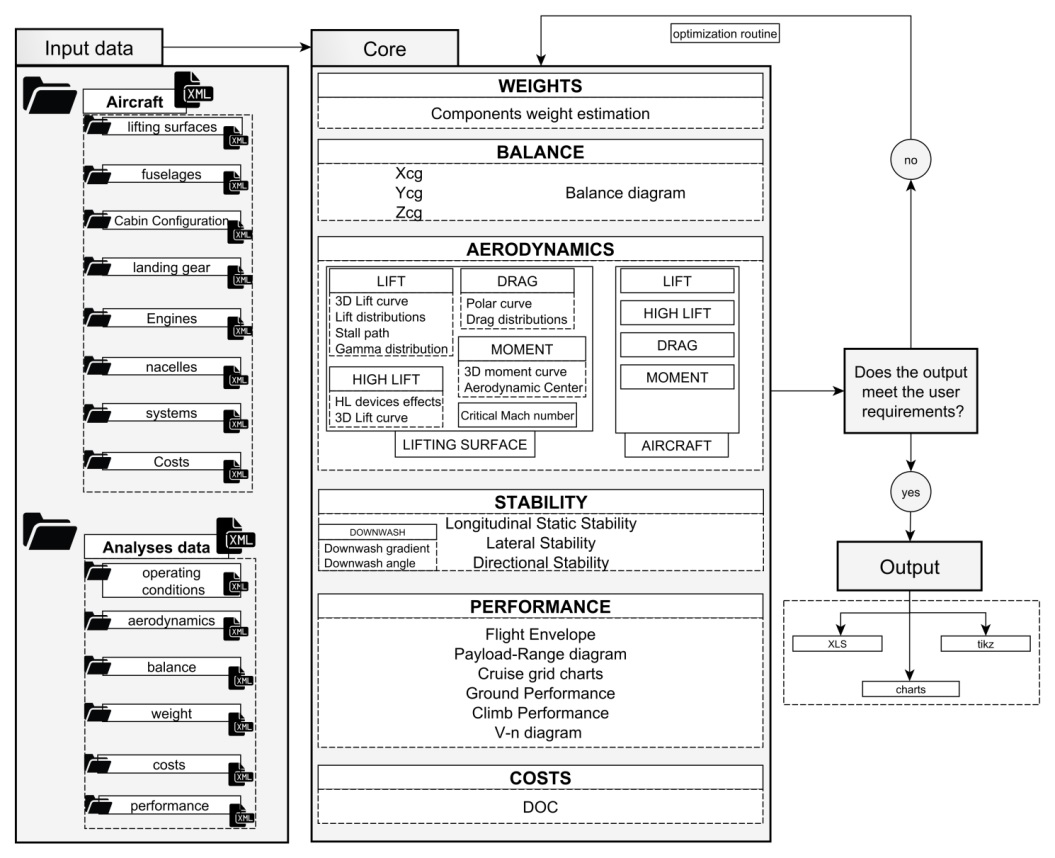
\includegraphics[height=0.45\textheight]{Immagini/Capitolo1/1_1-JPADSchematicFlowChart}
\caption[JPAD schematic flow-chart] {JPAD schematic flow-chart}
\label{JPADSchematicFlowChart}
\end{figure}

\begin{figure}[htbp] 
\centering
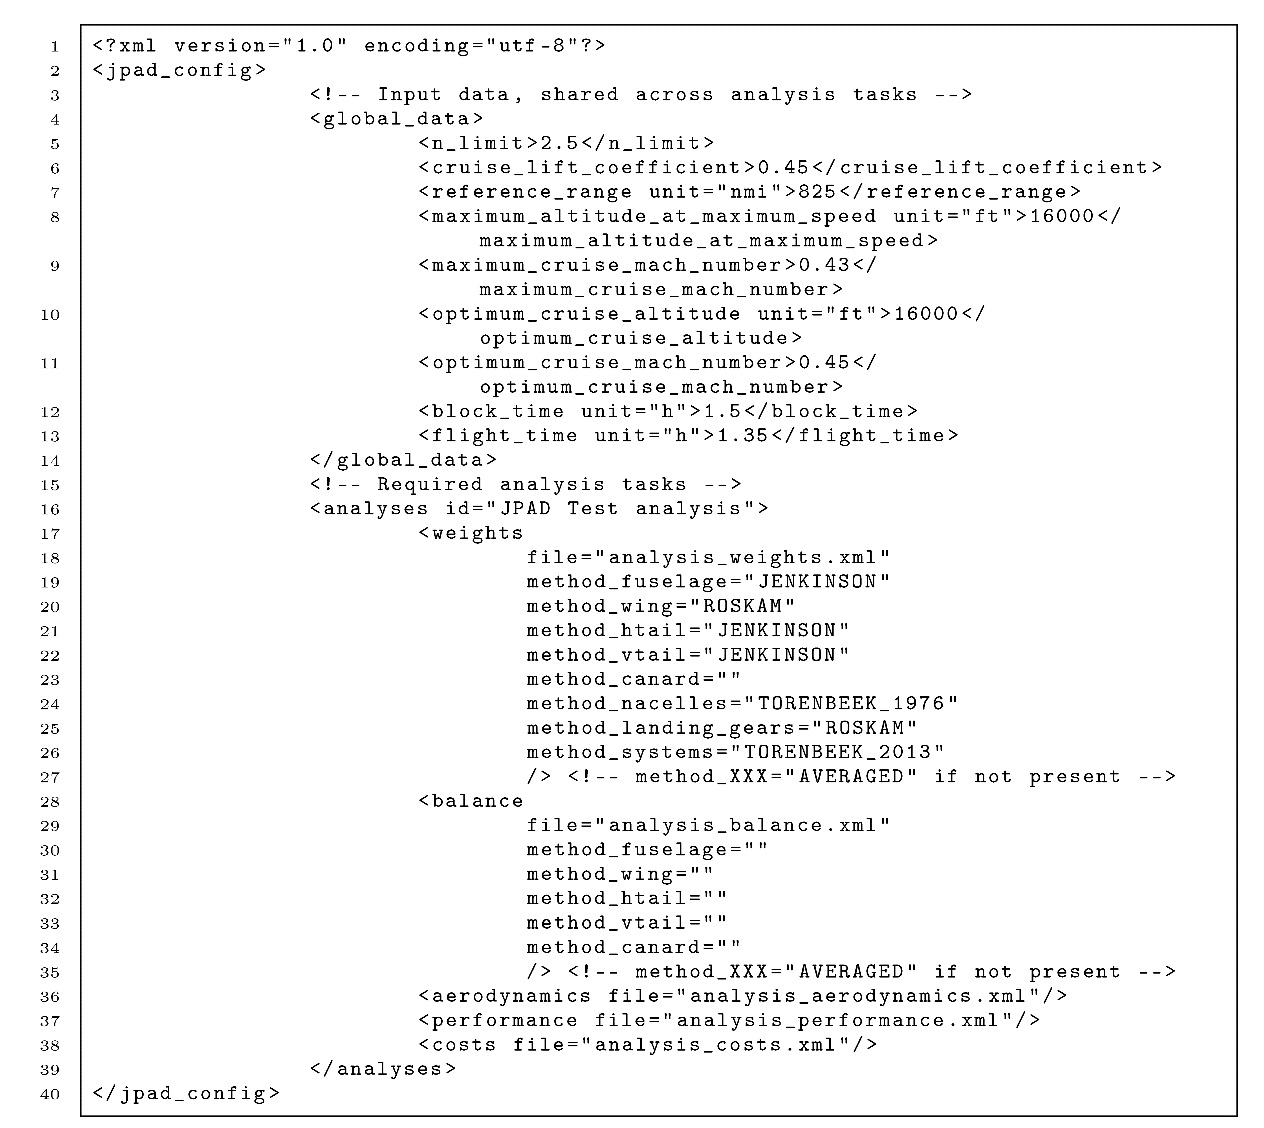
\includegraphics[height=0.45\textheight]{Immagini/Capitolo1/1_2-AnExampleOfTheAnalysisXmlFile}
\caption[Example of analysis.xml file] {An example of the analysis.xml file}
\label{AnExampleOfTheAnalysisXmlFile}
\end{figure}

\begin{figure}[htbp] 
\centering
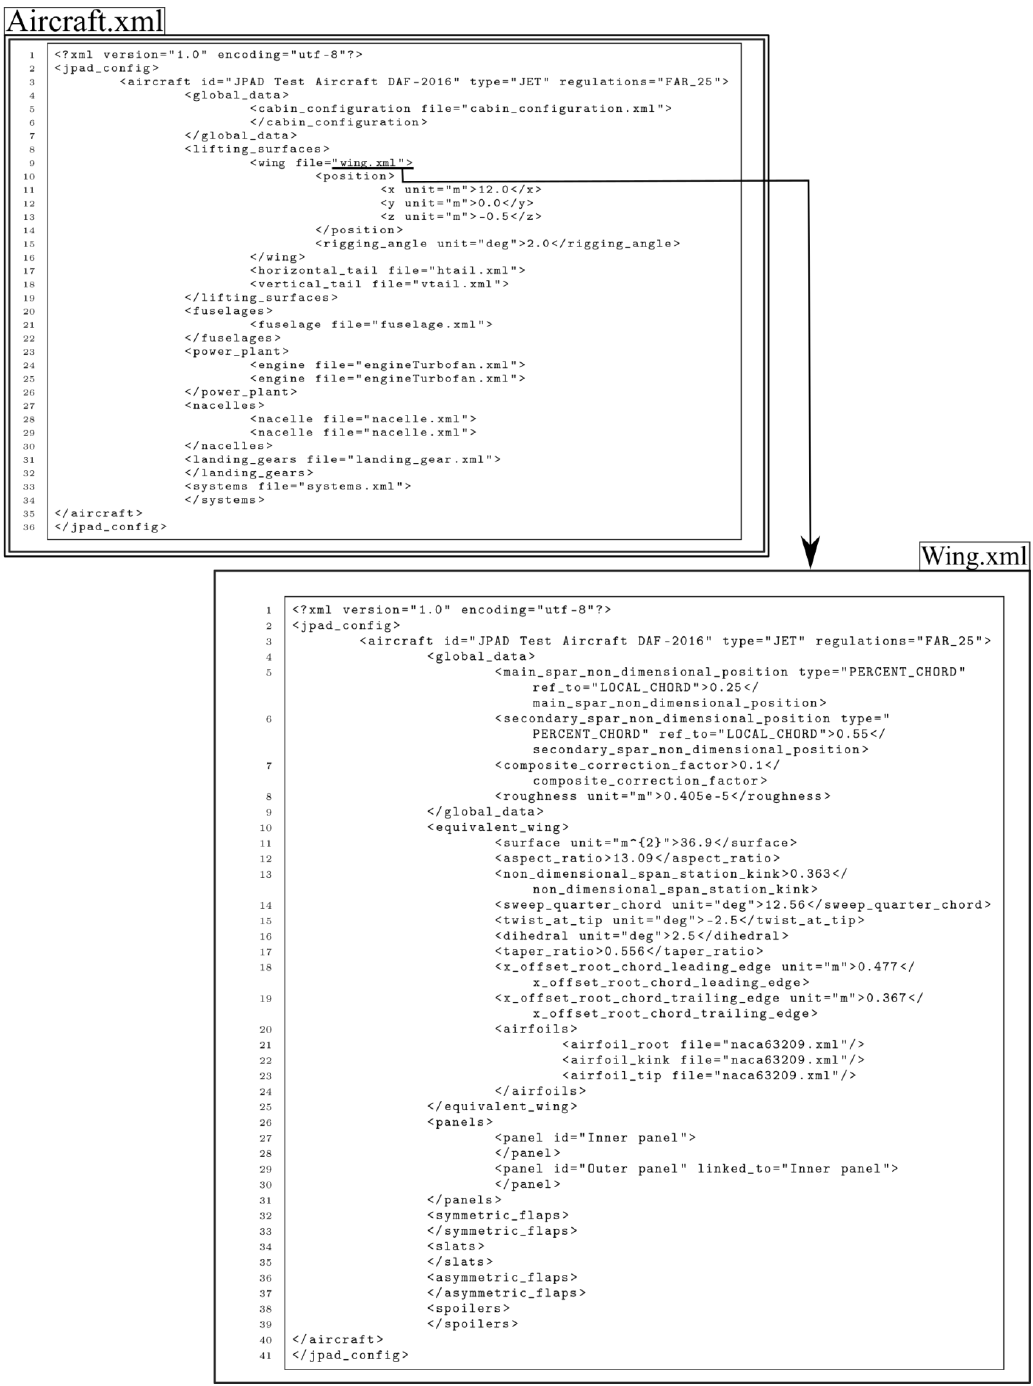
\includegraphics[width=\textwidth]{Immagini/Capitolo1/1_3-AnExtractFromAGeneralAircraftXmlInputFile}
\caption[Extract from general Aircraft.xml input file] {An extract from a general Aircraft.xml input file}
\label{AnExtractFromAGeneralAircraftXmlInputFile}
\end{figure}

The input block is defined by two main parts: aircraft and analyses definitions. The first one defines the aircraft model in parametric way using a main file (Aircraft.xml, see figure~\ref{AnExtractFromAGeneralAircraftXmlInputFile}) which collects all the components, linking them to their related XML file (i.e. fuselage.xml, vtail.xml, and so on) which contains all geometrical data.

The second one defines all necessary data for each analysis presents into core module (see figure~\ref{AnExampleOfTheAnalysisXmlFile}). Since the aircraft model contains only geometrical data, it is necessary to define several further data referred to each analysis. \\

The structure described above allows to generate different aircrafts, or different configurations of the same model, combining different components. The possibility to generate a series of different aircrafts in a simple and fast way, allows to easily perform comparisons between these latter. For example, assuming different wings and engines, it is possible to estimate the effects that some design parameters have on a specific output. Figure~\vref{FAR-25} shows how the FAR-25 take-off field length behaves with different values of the wing surface and the engine static thrust at fixed aircraft maximum take-off weight. This feature plays also a key role in the optimization process described in figure~\ref{JPADSchematicFlowChart}.

\begin{figure}[htbp] 
\centering
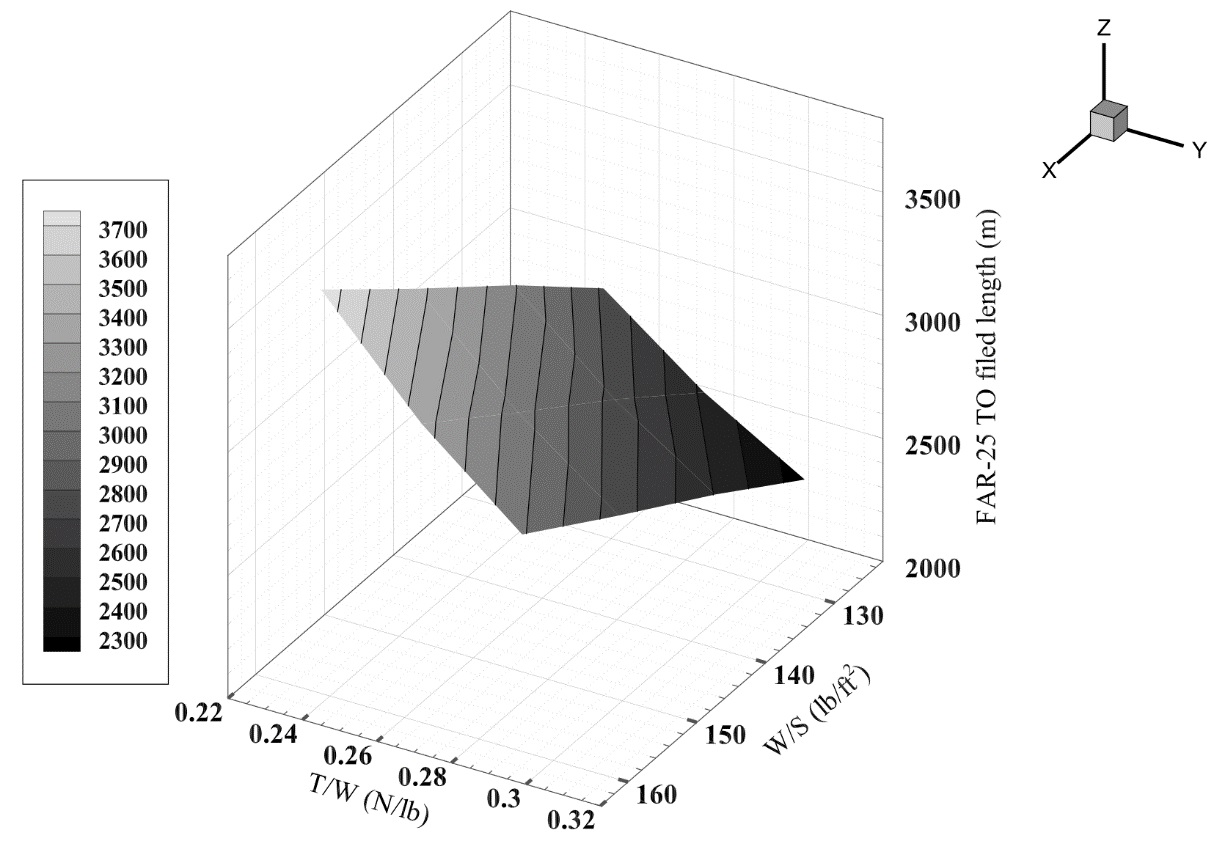
\includegraphics[width=\textwidth]{Immagini/Capitolo1/1_4-FAR-25TakeOffFieldLengthAtDifferentWingLoadingsAndThrustWeightRatios}
\caption[FAR-25 take-off field length at different $W/S_\text W$ and $T/W$] {FAR-25 take-off field length at different wing loadings and thrust-weight ratios}
\label{FAR-25}
\end{figure}

In the same way, it is possible to perform a complete analysis (those present into core block in figure~\ref{JPADSchematicFlowChart}), or a specific one, combining different analyses files. This allows an easier evaluation of generic cost function during optimization tasks, resulting in reduced amount of computational costs required for this kind of operations.

Besides the input, the second main block is the core, which manages all the available analyses. This contains several independent modules, as shown in the figure~\ref{JPADSchematicFlowChart}, that deals with following application fields.
\begin{itemize}
\item Weights: estimates the aircraft weight breakdown starting from a first guess maximum take-off weight and some mission requirements. In particular, it evaluates each aircraft component mass using well-known semi-empirical equations.
\item Balance: estimates the centre of gravity position related to each weight condition and draws the balance diagram.
\item Aerodynamics and Stability: the aerodynamics module estimates all the aerodynamic characteristics concerning lift, drag and moments coefficients at different operating conditions for each aircraft component (wing, tails, fuselage and nacelles), whereas the stability module gives useful data about static stability of the whole aircraft.
\item Performance: evaluates most important aircraft performance such as Payload-Range diagram, mission profile, cruise flight envelope, ground performance, climb performance and the cruise grid chart.
\item Costs: estimates the DOC (Direct Operating Costs) breakdown.
\end{itemize}

Finally, JPAD allows to obtain different kind of output: charts and data in XLS format.

% --------------------------------------------------------------------------------------------------------------------------------------------
% SEZIONE 2
% --------------------------------------------------------------------------------------------------------------------------------------------
\section{The Java Language}
\label{sec1.2}

Java was developed by Sun Microsystems, a company that was incorporated in Oracle from a few years. This programming language is a general-purpose, concurrent, class-based, object-oriented language. It is designed to be simple enough that many programmers can achieve fluency in the language \cite{javaoracle}.

One design goal of Java is portability, which means that programs written for the Java platform must run similarly on any combination of hardware and operating system with adequate runtime support. This is achieved by compiling the Java language code to an intermediate representation called Java bytecode, instead of directly to architecture-specific machine code. Java bytecode instructions are analogous to machine code, but they are intended to be executed by a virtual machine (VM) written specifically for the host hardware. End users commonly use a Java Runtime Environment (JRE) installed on their own machine for standalone Java applications, or in a web browser for Java applets \cite{wiki:java}. \\

There were five primary goals in the creation of the Java language \cite{java}:
\begin{itemize}
\item it must be ``simple, object-oriented, and familiar'';
\item it must be ``robust and secure'';
\item it must be ``architecture-neutral and portable'';
\item it must execute with ``high performance'';
\item it must be ``interpreted, threaded, and dynamic''.
\end{itemize}

Actually Java is the most used programming language according to TIOBE (see figure~\vref{TIOBE}). The TIOBE Programming Community index is an indicator of the popularity of programming languages. The ratings are based on the number of skilled engineers world-wide, courses and third party vendors.

\begin{figure}[htbp]
\centering
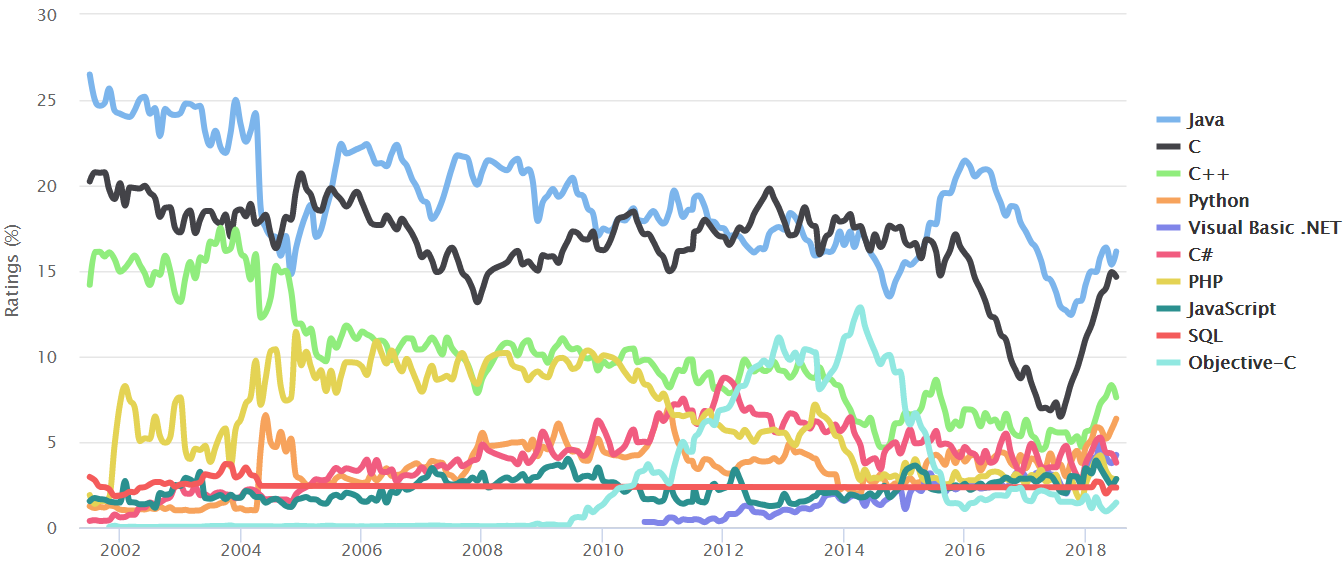
\includegraphics[width=\textwidth]{Immagini/Capitolo1/1_5-TrendTIOBE} 
\caption{TIOBE Programming Community index (\href{www.tiobe.com}{www.tiobe.com})}
\label{TIOBE}
\end{figure}

% --------------------------------------------------------------------------------------------------------------------------------------------
% SEZIONE 3
% --------------------------------------------------------------------------------------------------------------------------------------------
\section{Java choice}
\label{sec1.3}

The choice of Java as the programming language was driven by several considerations. These include the following:
\begin{itemize}
\item the language should be widely supported; this to avoid the case of many valid aircraft design applications and libraries that became obsolete due to the aging of the programming language used to build them;
\item the language is object oriented;
\item the language should promote the use of open source libraries, especially for I/O tasks and for complex mathematical operations;
\item the language and the companion Integrated Development Environment (IDE) should provide a widely supported Graphical User Interface (GUI) framework and a GUI visual builder;
\item the language should support and promote modularity.
\end{itemize}

The Java programming language meets all these requirements; moreover it is backed by Oracle and by a huge community of developers so it is continuously updated. Also, advanced and free IDEs (such as Eclipse) allow programmers to streamline and simplify the development process; in particular, the Eclipse IDE has been chosen to develop JPAD.

Being Java a pure object oriented programming language, it greatly encourages and simplifies modularization. Each module (package) can be programmed quite independently so that it is relatively easy to divide the work among several programmers. This is essential since the amount of classes and calculations needed to abstract, manage and analyse the entire aircraft is very large (presently the whole project counts more than 10 millions lines of code). For such a reason the establishment of common practices and the adherence to fundamental principle of software development (\emph{Don’t Repeat Yourself}, \emph{Separation of Concerns}, \emph{Agile software development}) are equally important.
% !TeX program = PdfLaTeX
% !TeX root = ../Main.tex

\chapter{Theoretical background}
\label{ch:ch2} %serve per citare il capitolo in un'altra sezione

Takeoff speeds are a safety key element for takeoff, and enable pilot situational
awareness and decision-making in this very dynamic situation. The use of erroneous
takeoff speeds can lead to tail strikes, high-speed rejected takeoff or initial climb with
degraded performance. 

% --------------------------------------------------------------------------------------------------------------------------------------------
% 								SEZIONE 1
% --------------------------------------------------------------------------------------------------------------------------------------------

\section{Take off speeds}
In this section a brief introduction to takeoff speeds will be provided \cite{Airbus:Flight:Notes}. \\
In aviation, these speeds are standard terms used to define airspeeds important or useful to the operation of all aircraft. They are derived from data obtained by aircraft designers and manufacturers during flight testing and verified in most countries by government flight inspectors during aircraft type-certification testing. Using them is considered a best practice to maximize aviation safety, aircraft performance or both. Takeoff speeds are calculated prior to a take off in accordance with aircraft weight, environmental factors etc.

\begin{figure}[htbp]
	\centering
	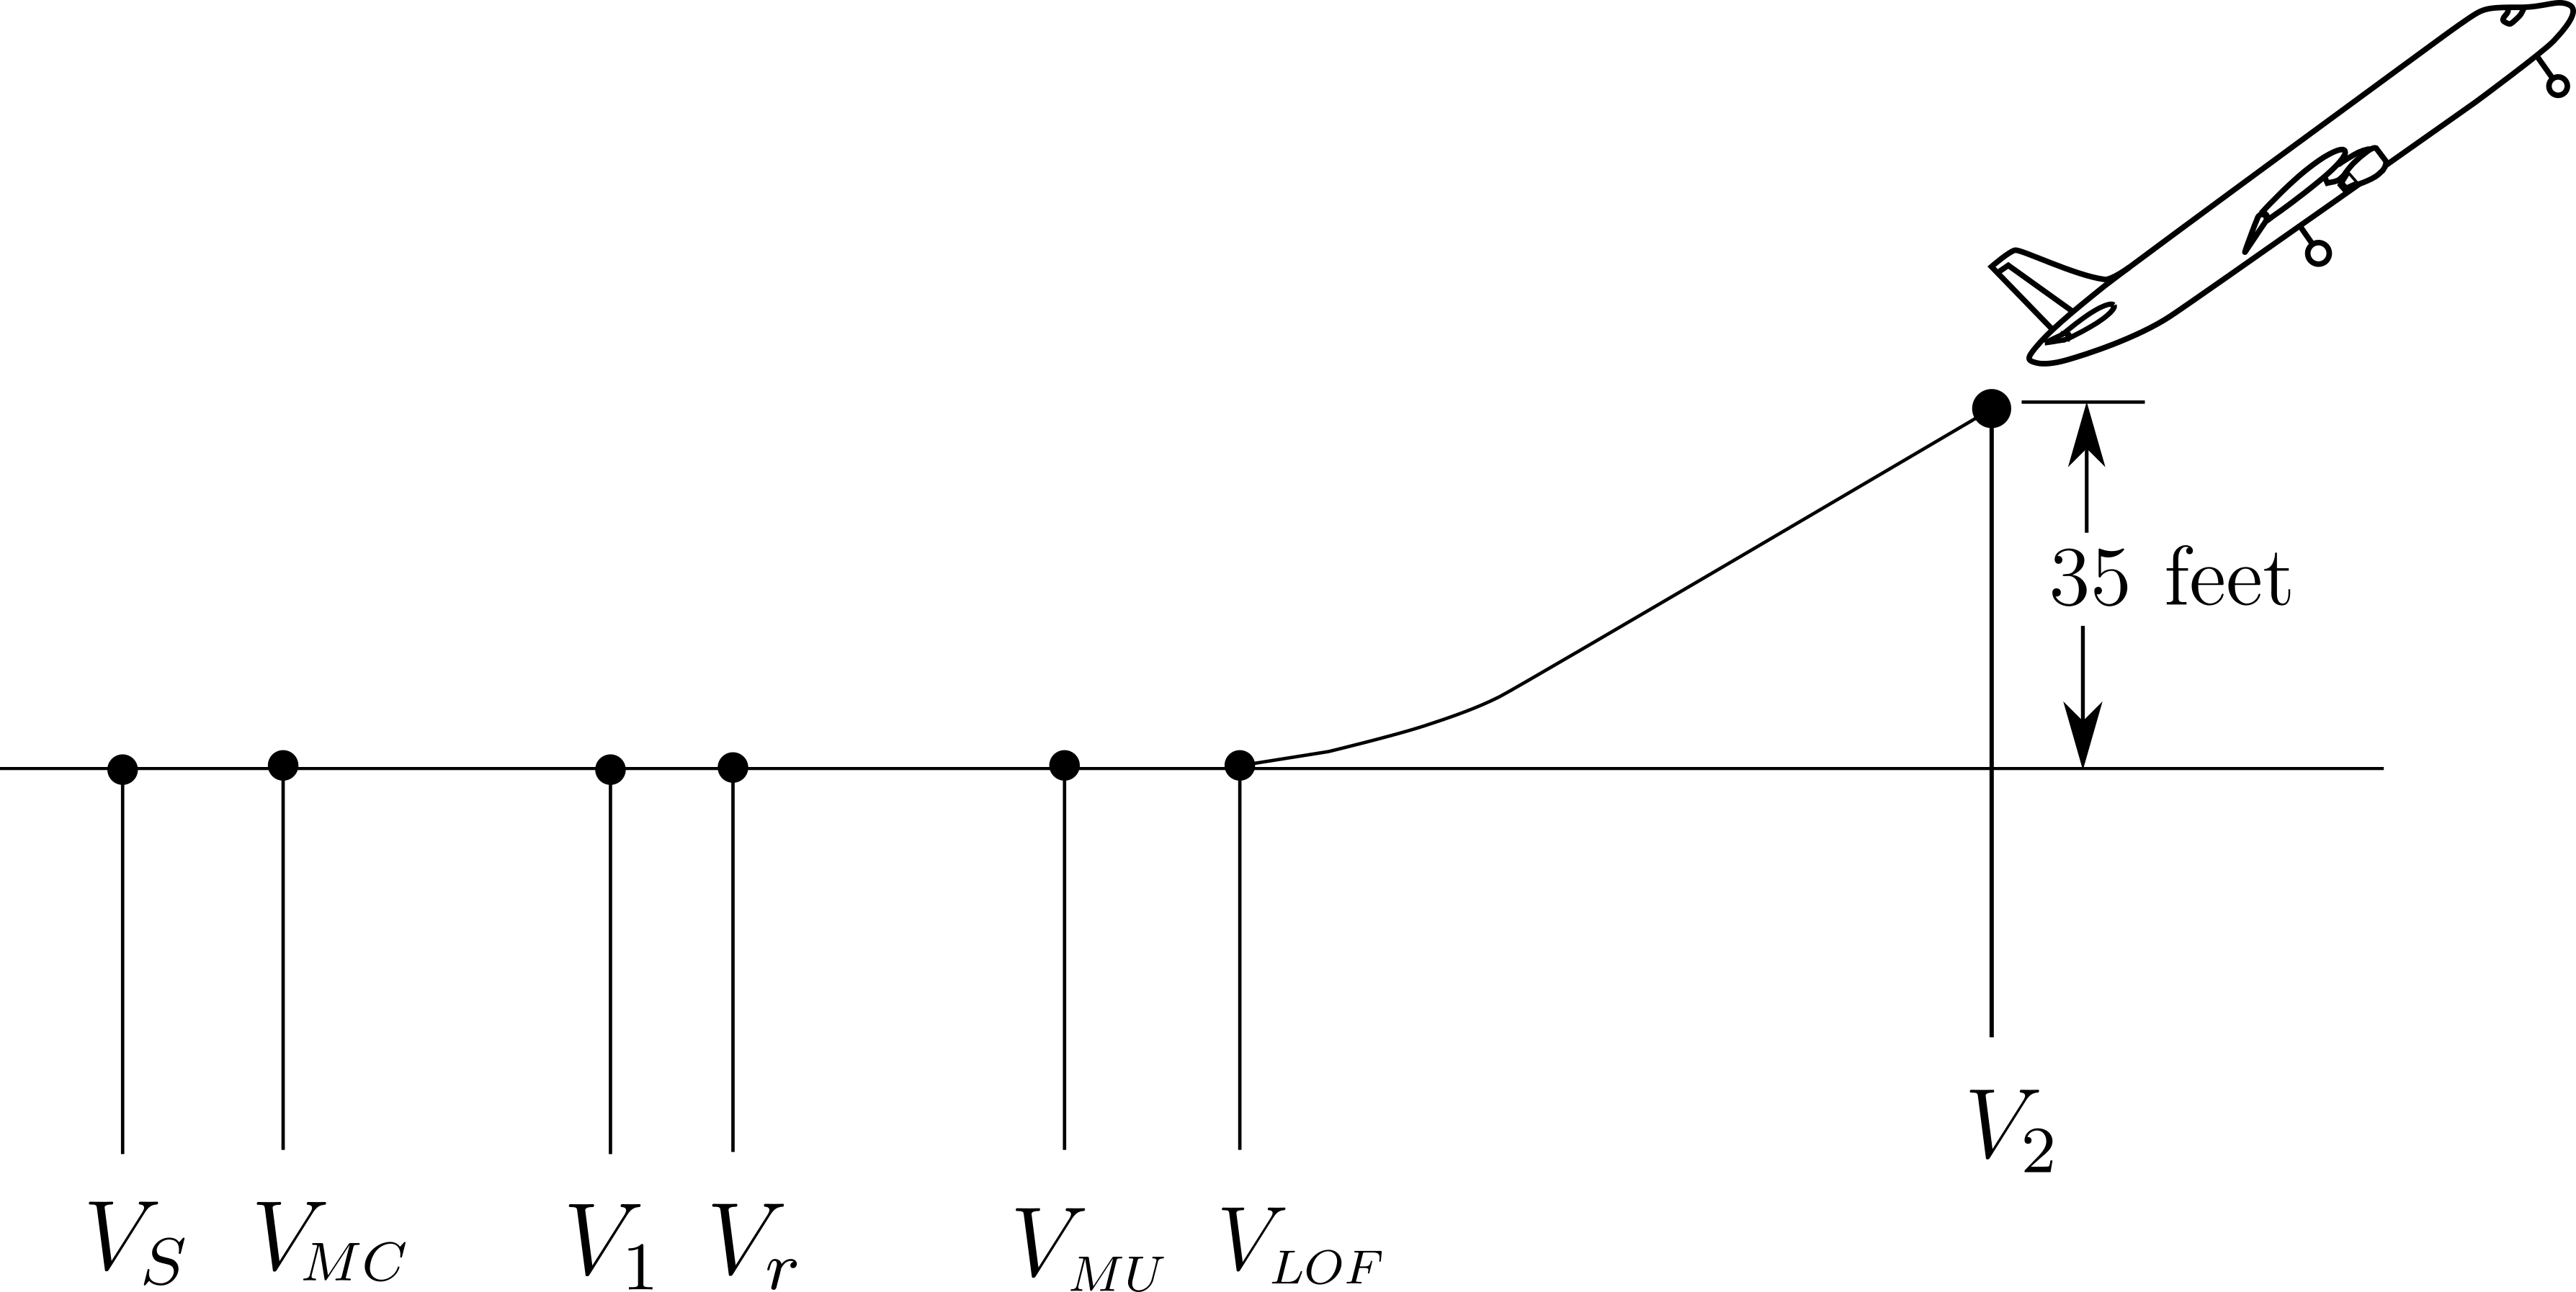
\includegraphics[height=7cm, keepaspectratio ]{Immagini/Capitolo2/takeoffSpeeds} 
	\caption{Takeoff speeds} % didascalia
	\label{fig:figura2_4} % etichetta per citarla nel testo
\end{figure}

\subsubsection{Velocity of stall $V_{S}$}
Aircraft stall speed during take off run.

\subsubsection{Velocity of Minimum Control $V_{MC}$}
During the takeoff roll, it is of utmost importance to know the minimum speed at which
the aircraft will remain controllable, in the event of an engine failure on ground. This is
because, in such a case, and if the takeoff is continued, only the rudder will be able to
counteract the yaw moment that is generated by asymmetric engine(s) thrust.
According to current regulations, the minimum speed at which an aircraft is defined to be “controllable”
(lateral excursion lower than 30 feet) after an engine failure on ground, is referred to
as $V_{MC}$ (Velocity of Minimum Control on Ground). 

\subsubsection{Decision Speed $V_1$}
$V_1$ is the maximum speed at which a rejected takeoff can be initiated, in the event of an
emergency. $V_1$ is also the minimum speed at which a pilot can continue a takeoff after an engine
failure.
If an engine failure is detected after $V_1$, the takeoff must be continued. This implies that
the aircraft must be controllable on ground. Therefore, V1 is always greater than $V_{MC}$.

\subsubsection{Rotation speed $V_r$}
Speed at which planes with a tricycle trolley lift the front wheel off the ground during take off.
 
\subsubsection{Velocity of Minimum Unstick $V_{MU}$}
 $V_{MU}$ is achieved by pitching the aircraft up to the maximum (tail on the runway, for
aircraft that are are geometrically-limited) during the takeoff roll (Refer to Figure~\ref{fig:figura2_1}). The speed at which the aircraft first lifts off is  $V_{MU}$. Therefore, lift-off is not
possible prior to  $V_{MU}$. 

\begin{figure}[htbp]
	\centering
	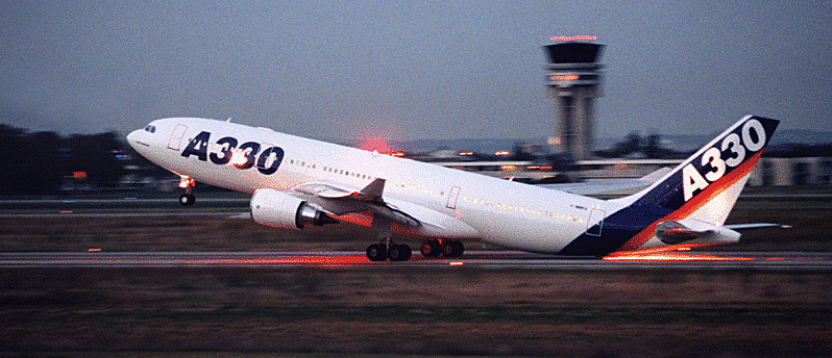
\includegraphics[height=6cm, keepaspectratio ]{Immagini/Capitolo2/2_1-VMUFlightTestOnAnA330} 
	\caption{$V_{MU}$ Flight Test on an Airbus A330} % didascalia
	\label{fig:figura2_1} % etichetta per citarla nel testo
\end{figure}

\subsubsection{Lift-off speed $V_{LOF}$}
Effective take off speed. It is assessed by adding a 10\% to the Minimum unstick speed with all the operating engines or a 5\% with an inoperative engine.

\subsubsection{Takeoff safety speed $V_2$}
$V_2$ is the speed at which the aircraft may safely be climbed with one engine inoperative. This speed is nicknamed a “take off safety speed”; it is the speed an aircraft with one engine inoperative must be able to attain in order to leave the runway and get 35 feet off the ground at the end of the runway, maintaining a 200 ft/min climb thereafter. This is the lowest speed at which the aircraft complies with the handling criteria associated with a climb after a take off, followed by the failure of an engine.

% --------------------------------------------------------------------------------------------------------------------------------------------
% 								SEZIONE 2	
% --------------------------------------------------------------------------------------------------------------------------------------------

\section{Ground effect}
Due to the fact that during the takeoff the aircraft is on the ground, in order to asses $V_{MU}$,  it is important to consider the ground effect. This generally become measurable at a height above the ground of one wing-span and increase in magnitude as the height above the ground decreases. Both theoretical and
experimental investigations indicate that ground proximity produces an increase in the lift-curve
slope, a decrease in drag, and a reduction of nose-up pitching moment for most aircraft planforms in
the clean configuration. However, high-lift configurations deviate from this trend in that the ground
effect tends to reduce the lift-curve slope \cite{Datcom}.\\

The majority of the theoretical approaches analyzing ground effects employ an image-vortex theory
to represent the ground plane. The salient aspects of this theory are discussed below.\\

Away from the ground plane, the downwash of the two trailing vortices contributes to the wing
drag die to lift by rotating the force vector rearward.\\
However, near the ground plane, the trailing vortices of the image vortex system have an upwash component.\\

This upwash velocity component reduces the downward rotation of the flow direction caused by the wing trailing vortices, thus decreasing the wing drag due to lift.\\

The ground effects on lift are determined somewhat by the planform of the configuration. For
low-aspect-ratio delta configurations, the general trend is a constant increase in $C_L$ due to ground
effect, as shown in figure~\ref{fig:figura2_2}.
However, transport-type configurations show quite a different trend, as presented in figure~\ref{fig:figura2_3}.\\
This trend is dependent upon tie type of high-lift system employed.

\begin{figure}[htbp]
	\centering
	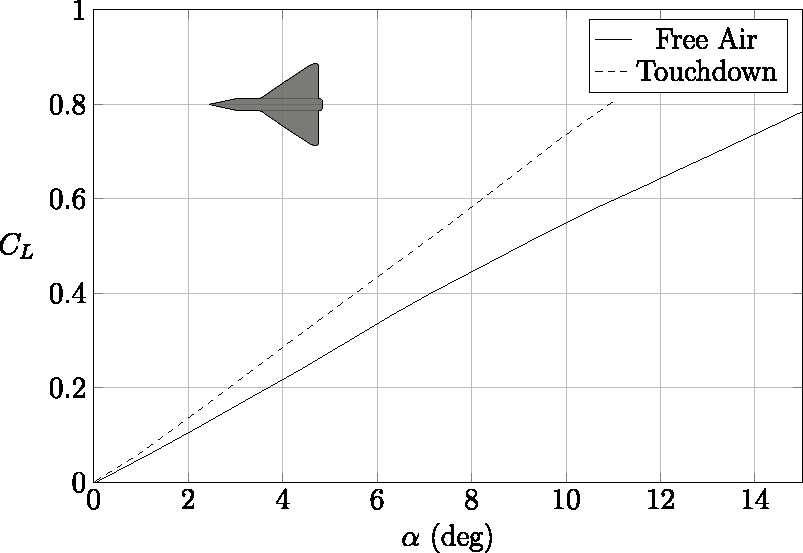
\includegraphics[height=10cm, keepaspectratio ]{Immagini/Capitolo2/2_2-GroundEffectDeltaConf} 
	\caption{Ground effect on 55°  delta configuration} % didascalia
	\label{fig:figura2_2} % etichetta per citarla nel testo
\end{figure}

\begin{figure}[htbp]
	\centering
	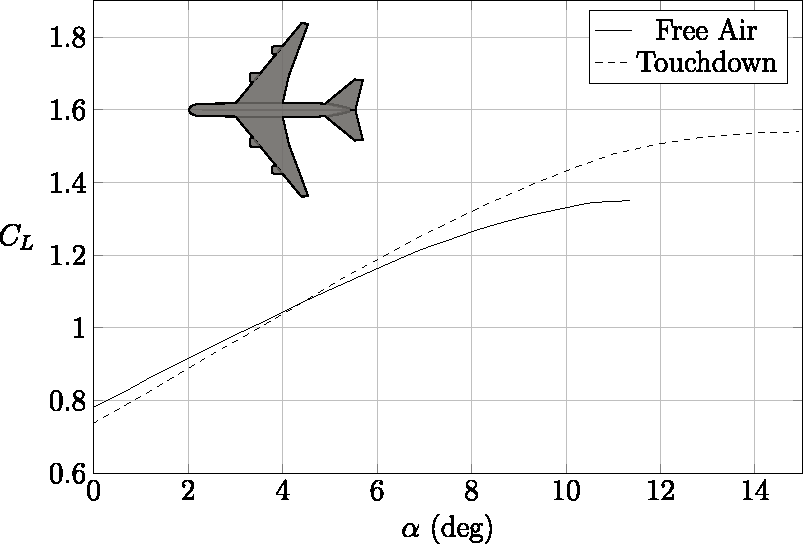
\includegraphics[height=10cm, keepaspectratio ]{Immagini/Capitolo2/2_3-GroundEffectJetTranspConf} 
	\caption{Ground effect on a jet transport configuration} % didascalia
	\label{fig:figura2_3} % etichetta per citarla nel testo
\end{figure}

\section{Datcom methods}
\label{sec:sec3}
For most vehicles, calculating the change in lift due to ground effects consists of evaluating two
components:
 \begin{enumerate}
 \item the change in wing-body lift;
 \item the change in tail-body lift due to the effects of downwash.
 \end{enumerate}
 
The change in tail-body lift due to the presence of the ground is generally small in comparison to
the downwash effects and is neglected in the Datcom methods.\\
Both of the Datcom methods presented require the user to construct wing-body and tail-body lift
curves in ground effect based on their corresponding free-air lift curves. Equations are given that
calculate the change in angie of attack due to ground effect at a constant lift coefficient. The
ground-effect lift curves are then constructed by shifting the free-air lift curves at every $C_L$ by the
corresponding increment in angle of attack due to ground effect at constant lift coefficients.

\begin{figure}[htbp]
	\centering
	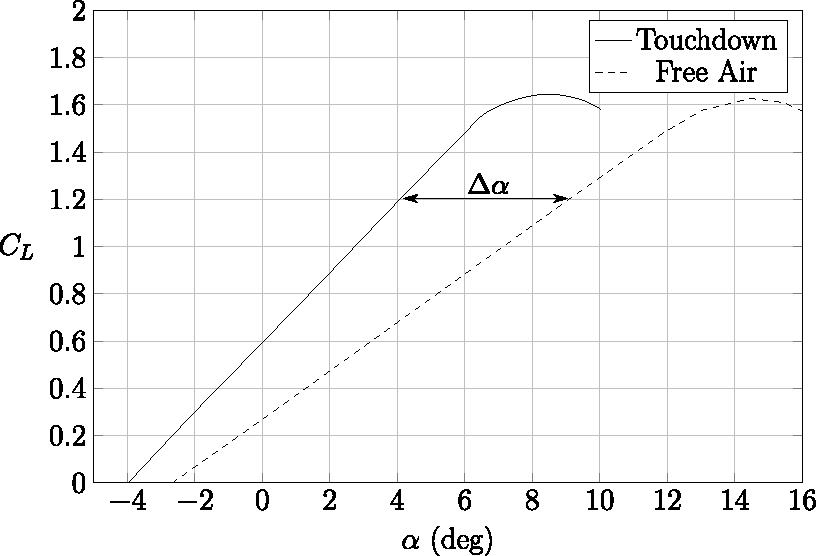
\includegraphics[height=10cm, keepaspectratio ]{Immagini/Capitolo2/disegno} 
	\caption{Ground effect on a jet transport configuration} % didascalia
	\label{fig:figura2_3_1} % etichetta per citarla nel testo
\end{figure}

\subsubsection{Method I}
This method estimates the ground effects on lift in the linear-lift range for a subsonic transport
configuration. It includes the effects of taper ratio, sweep-back, dihedral, and flap deflection, while neglecting the effects of
wing thickness since they are generally small. The wing-flap effects are valid only for split and slotted flaps as they are accounted for by empirical curves. \\
The change in wing-body angle of attack at a constant lift coefficient due to ground effect with
respect to the out-of-ground-effect lift curve is given by:

\begin{equation}
\begin{split}
\left(\Delta \alpha\right)_G=&-\left[\frac{9.12}{\AR}+7.16\left(\frac{c_r}{b}\right)\right]\left( C_{L_f} \right)_{WB}x \ +\\
&-\frac{\AR}{2\left( C_{L_{\alpha}} \right)_{WB}}\left(\frac{c_r}{b}\right)\left(\frac{L}{L_0}-1\right)\left( C_{L_f} \right)_{WB}r \ + \\ &-\frac{\left(\delta_f /50\right)^2}{\left( C_{L_{\alpha}} \right)_{WB}}\Delta \left(\Delta C_L \right)_{flap} \ \text{(per  deg)}
\label{eq:equazione2_1} % etichetta per citarla nel testo
\end{split}
\end{equation}
\\ \\ \\ \\  where\\ \\ \\
\begin{tabulary}{1\textwidth}{L L}
\begin{minipage}[T]{6cm}$\Delta \left(\Delta C_L \right)_{flap}$  \end{minipage}& is an empirical factor to account for the effect of flaps and is obtained from~\vref{fig:figura2_4} as a function of the height of the quarter-chord point of the wing root chord above the ground,\\ \\
\AR & is the wing aspect ratio, \\ \\
$\dfrac{c_r}{b}$ & is the ratio of wing root chord to wing span, \\ \\
$\left( C_{L_f} \right)_{WB} $ & is the wing-body lift coefficient including flap effects, out of ground effect, \\ \\
$x$ & accounts for the effects on lift due to the image trailing vortex and is obtained
from~\vref{fig:figura2_6} as a function of wing geometry and the wing height above
the ground, \\ \\
$\dfrac{L}{L_0}-1 $ & accounts for the effects on lift due to the image bound vortex and is obtained from~\vref{fig:figura2_8} as a function of wing geometry, lift coefficient, and the height of the quarter-chord point of the wing root chord above the ground. \\ \\
$\left( C_{L_{\alpha}} \right)_{WB} $  & is the wing body lift-curve slope, per degree, out of  ground effect \\ \\
$r$ & accounts for the effect of finite span and is obtained from~\vref{fig:figura2_9} as a function of wing height above the ground, \\ \\
\end{tabulary}

The first term in Equation~\ref{eq:equazione2_1} accounts for the effects of he trailing vortex, the second term for the effects of the trailing vortex, the second term for the effects of the bound vortex, and the third term for wing-flap effects. The method does not account for the effects of wing-leading-edge devices.\\
\begin{figure}[H]
	\centering
	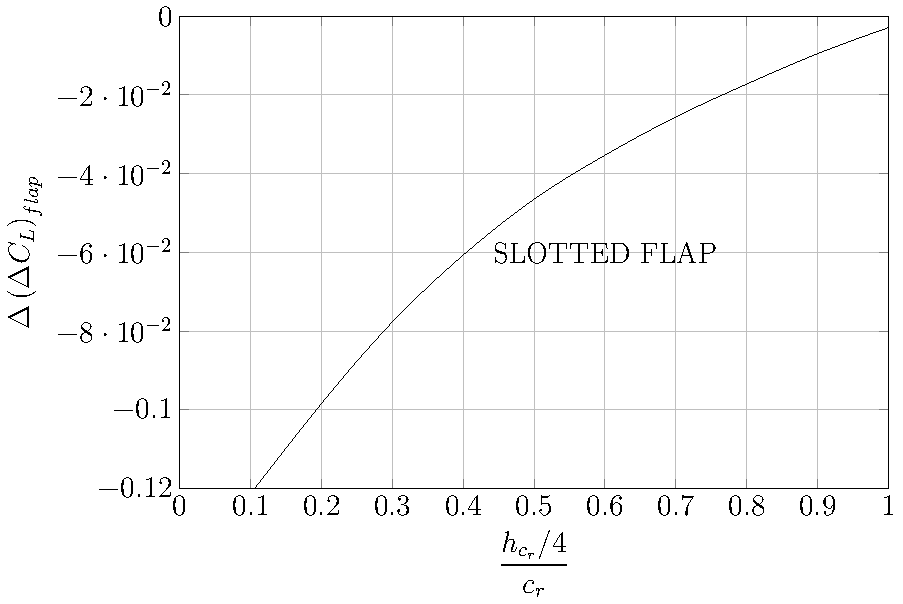
\includegraphics[height=7.3cm, keepaspectratio ]{Immagini/Capitolo2/2_4-Delta_alpha_CL_Ground_Effect_DeltaDelta_CL_flap_vs_h_cr_4_cr} 
	\caption{Effect of flap deflection on the ground influence on lift} % didascalia
	\label{fig:figura2_4} % etichetta per citarla nel testo
\end{figure}

\begin{figure}[H]
	\centering
	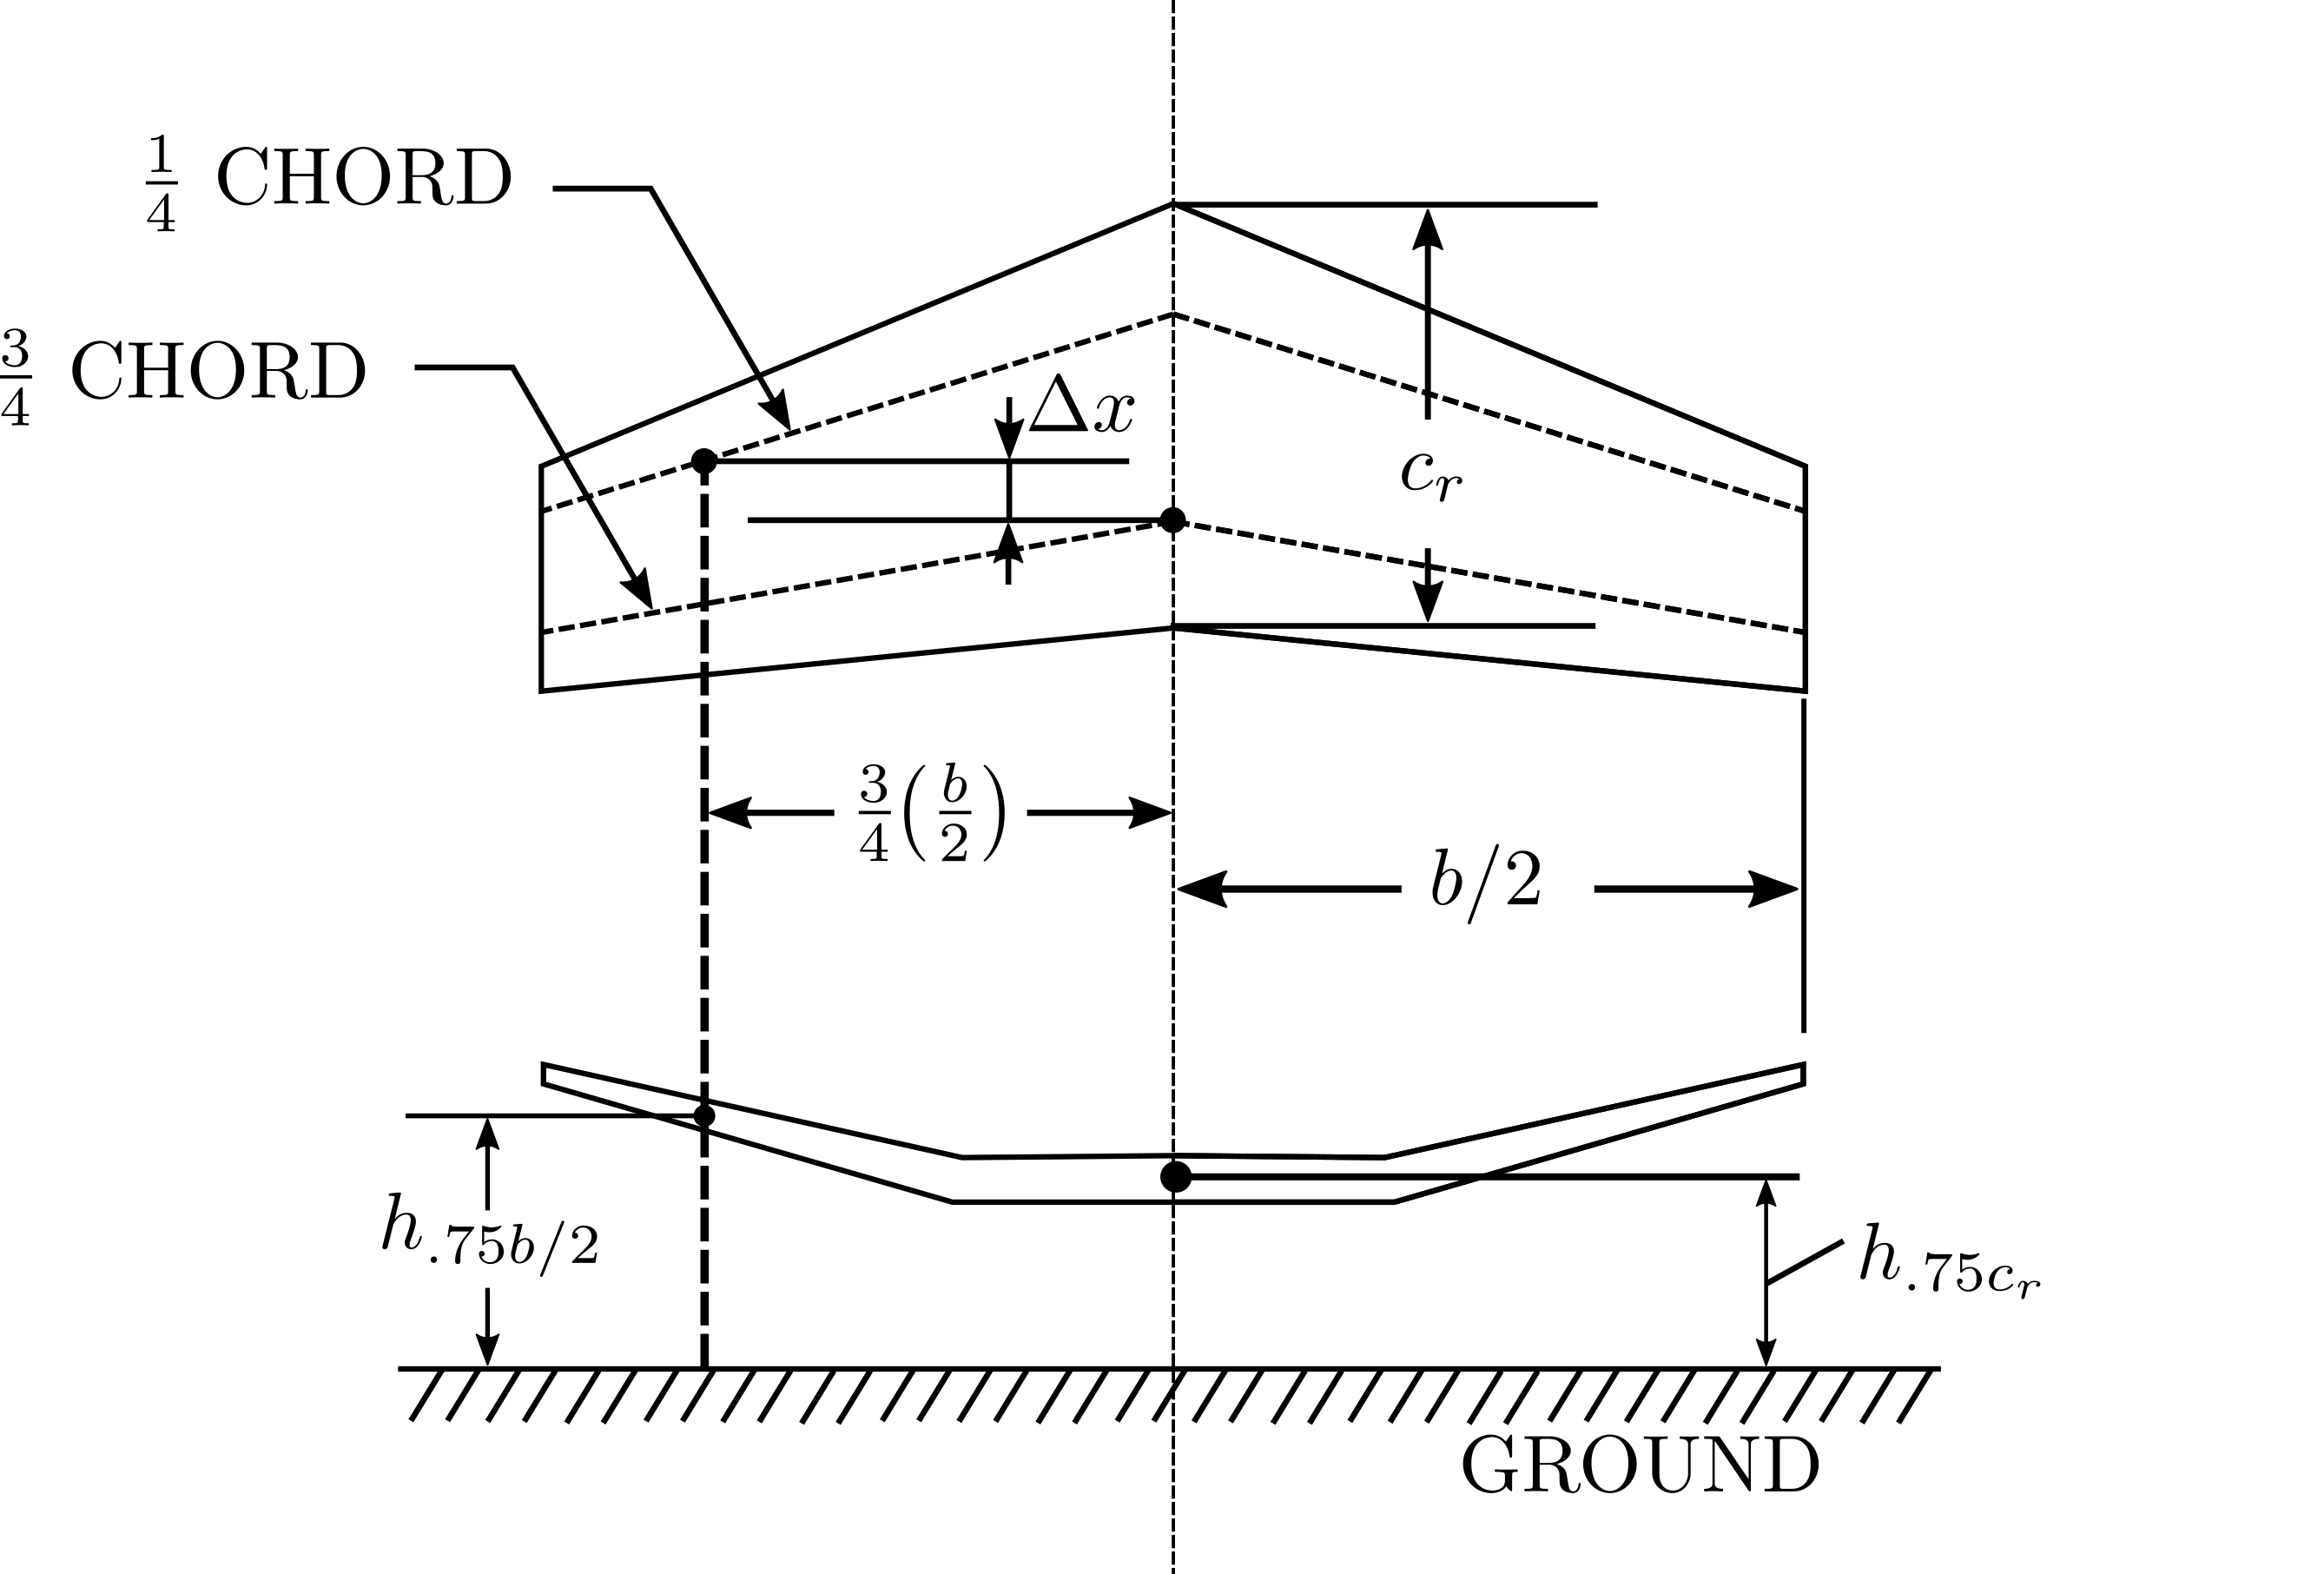
\includegraphics[height=9cm, keepaspectratio ]{Immagini/Capitolo2/disegno-1} 
	\caption{Description of geometric parameters} % didascalia
	\label{fig:figura2_5} % etichetta per citarla nel testo
\end{figure}

where
\[\frac{h}{b/2}=\frac{0.5\left(h_{.75b/2}+h_{.75c_r}\right)}{b/2}\]

\begin{figure}[H]
	\centering
	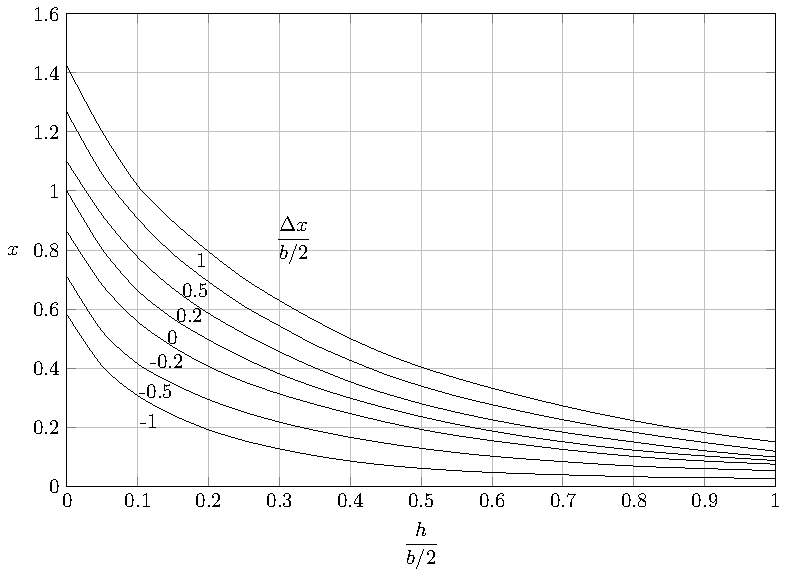
\includegraphics[height=9.5cm, keepaspectratio ]{Immagini/Capitolo2/2_6-(Delta_alpha_CL_Ground_Effect)_x_vs_2hfracb_Deltax} 
	\caption{Parameter accounting for ground effect on lift due to trailing vortices} % didascalia
	\label{fig:figura2_6} % etichetta per citarla nel testo
\end{figure}


\begin{figure}[H]
	%\centering
	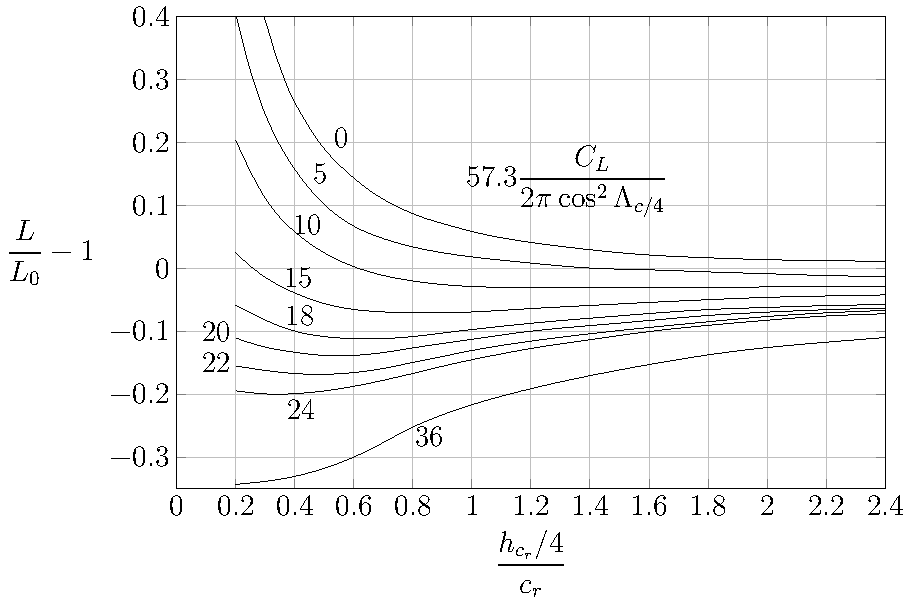
\includegraphics[height=8.5cm, keepaspectratio ]{Immagini/Capitolo2/2_8-Delta_alpha_CL_Ground_Effect_L_L0_minus1_vs_h_cr_4_cr} 
	\caption{Parameter accounting for ground effect on lift due to bound vortices} % didascalia
	\label{fig:figura2_8} % etichetta per citarla nel testo
\end{figure}

\begin{figure}[H]
	\centering
	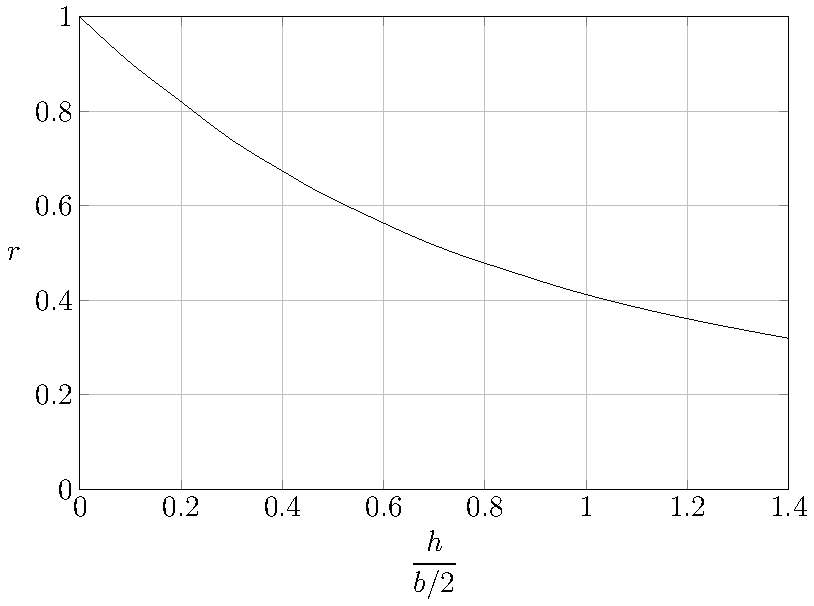
\includegraphics[height=8.5cm, keepaspectratio ]{Immagini/Capitolo2/2_9-Delta_alpha_G_r_vs_2hfracb} 
	\caption{Factor accounting for finite span in ground effect} % didascalia
	\label{fig:figura2_9} % etichetta per citarla nel testo
\end{figure}

In the linear-lift region, the change in downwash (a decrease) on this tail-body due to ground effects
is derived theoretically by representing the ground plane as an image-vortex system.\\
The change (a decrease) in tail-body downwash due to ground effects in the linear-lift range is given by:

\begin{equation}
\left(\Delta \varepsilon \right)_G=\varepsilon \left[\frac{b_{eff}^2+4\left(H_H+H\right)^2}{b_{eff}^2+4\left(H_H-H\right)^2}\right]
\label{eq:equazione2_2} % etichetta per citarla nel testo
\end{equation}
where \\ \\

\begin{tabulary}{1\textwidth}{L L}
\begin{minipage}[T]{3cm}$\left(\Delta \varepsilon \right)_G$  \end{minipage}& is the difference between the downwash in free air and the downwash in
ground effect,\\ \\
$\varepsilon$ & is the downwash out of ground effect, \\ \\
$H$ & is the height of $\frac{\overline c}{4}$ of the wing above the ground, \\ \\
$H_H$ & is the height of $\frac{\overline c}{4}$ of the horizontal tail above the ground.\\ \\
$b_{eff}$ & is the effective wing span defined as\\ \\
\end{tabulary}

\begin{equation}
b_{eff}=\frac{ C_{L_{WB}} +\Delta C_{L_f} }{\dfrac{ C_{L_{WB}} }{b'_W}+ \dfrac {\Delta C_{L_f} }{b'_f}}
\label{eq:equazione2_2_1} % etichetta per citarla nel testo
\end{equation}
  \indent \indent \indent  where \\ \\

\begin{tabulary}{1\textwidth}{L L}
\begin{minipage}[T]{4cm}$\qquad \qquad  C_{L_{WB}}$  \end{minipage}&  is the wing-body lift coefficient, flaps retracted, out of ground effect,\\ \\
$\qquad \qquad  \Delta C_{L_f}$ & is the change in lift coefficient due to flaps, out of ground effect. \\ \\
\end{tabulary}

\begin{equation}
b'_W=\left(\frac{b'_W}{b}\right)b
\label{eq:equazione2_3_1} % etichetta per citarla nel testo
\end{equation}

\begin{equation}
b'_W=\left(\frac{b'_f}{b'_W}\right)\left(\frac{b'_W}{b}\right)b
\label{eq:equazione2_3_2} % etichetta per citarla nel testo
\end{equation}
 \indent \indent \indent The ratio $\dfrac{b'_W}{b}$ is given in~\vref{figura2_10} as a function of taper \indent \indent \indent ratio and aspect ratio, and $\dfrac{b'_f}{b'_W}$ is given in~\vref{fig:figura2_11} as   \indent \indent \indent a function of the  ratio  of flap span to wing span.\\
 
The horizontal-tail lift curve in ground effect is constructed by shifting the free-air lift curve at
every $C_L$ by the corresponding \(-\left(\Delta \varepsilon \right)_G\), i.e.,
\begin{equation}
\left(\Delta \alpha_H \right)_G=-\left(\Delta \varepsilon \right)_G
\label{eq:equazione2_3} % etichetta per citarla nel testo
\end{equation}

 \begin{figure}[H]
	%\centering
	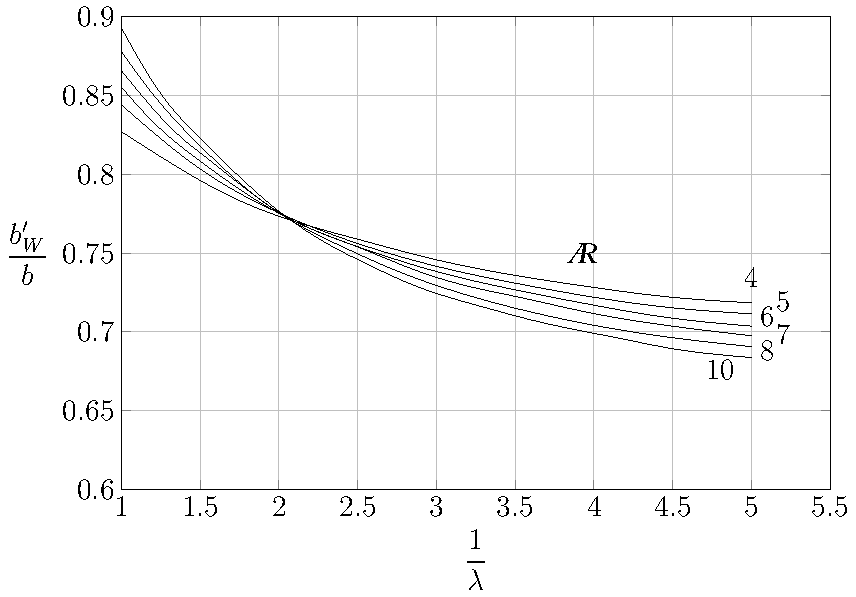
\includegraphics[height=10.5cm, keepaspectratio ]{Immagini/Capitolo2/2_10-bapexwfracb} 
	\caption{Effective wing span in the presence of the ground} % didascalia
	\label{figura2_10} % etichetta per citarla nel testo
\end{figure}

\begin{figure}[H]
	\centering
	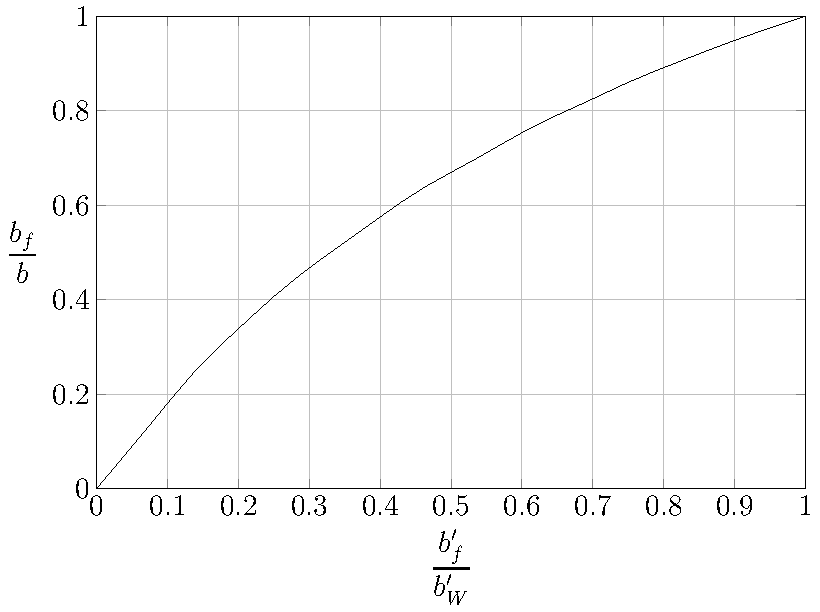
\includegraphics[height=10.5cm, keepaspectratio ]{Immagini/Capitolo2/2_11-bapexffracbapexw} 
	\caption{Effective flap span in the presence of the ground} % didascalia
	\label{fig:figura2_11} % etichetta per citarla nel testo
\end{figure}

\subsubsection{Method II}
This method estimates the ground effects on wing-body lift in the linear-lift range for all
configurations not included in Method I.
The change in wing-body angle of attack due to ground
effects with respect to the out-of-ground-effect lift curve is given by:

\begin{equation}
\left(\Delta \alpha\right)_G=-18.4\frac{\left( C_{L_f} \right)_{WB}\sigma}{\AR}+rT\frac{\left( C_{L_f} \right)_{WB}^2}{57.3\left( C_{L_{\alpha}} \right)_{WB}}-rB+K\left(\frac{t}{c}\right)_{max} \ \text{(per  deg)}
\label{eq:equazione2_4} % etichetta per citarla nel testo
\end{equation}
\\ \\   where\\ \\ \\
\begin{tabulary}{1\textwidth}{L L}
\begin{minipage}[T]{6cm}$\sigma$  \end{minipage}& is Prandtl's interference coefficient from multiplane theory and is obtained from~\vref{fig:figura2_12} as a function of wing height above the ground,\\ \\
$r$ & accounts for the effect of finite span and is obtained from~\vref{fig:figura2_9} as a function of wing height above the ground, \\ \\
$T$ & accounts for the reduction of the longitudinal velocity and is obtained from~\vref{fig:figura2_13} as a function of wing height above the ground, \\ \\
$B$ &accounts for the change in circulation and is obtained from~\vref{fig:figura2_14} as a function of wing height above the ground, \\ \\
$K$ & accounts for the effective wing thickness and is obtained from~\vref{fig:figura2_15} as a function of wing height above the ground, \\ \\
$\left(C_{L_{\alpha}} \right)_{WB}$ & is the wing-body lift-curve slope, per degree, out of ground effect, \\ \\
$\left(\dfrac{t}{c}\right)_{max}$  & is the ratio of maximum wing thickness to wing chord, \\ \\
$\left( C_{L_f} \right)_{WB}$ & is the wing-body lift coefficient including flap effects, out of ground effect. \\ \\
\end{tabulary}

\begin{figure}[H]
	\centering
	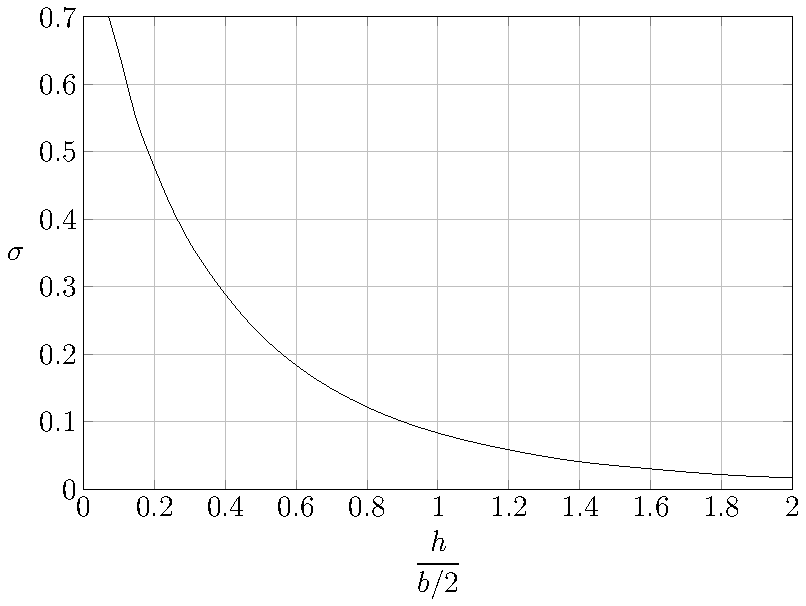
\includegraphics[height=10.5cm, keepaspectratio ]{Immagini/Capitolo2/2_12-(Delta_alpha_G)_sigma_vs_2hfracb} 
	\caption{Prandtl's interference coefficient - indicative of variation in induced vertical velocity with ground effect} % didascalia
	\label{fig:figura2_12} % etichetta per citarla nel testo
\end{figure}

\begin{figure}[H]
	\centering
	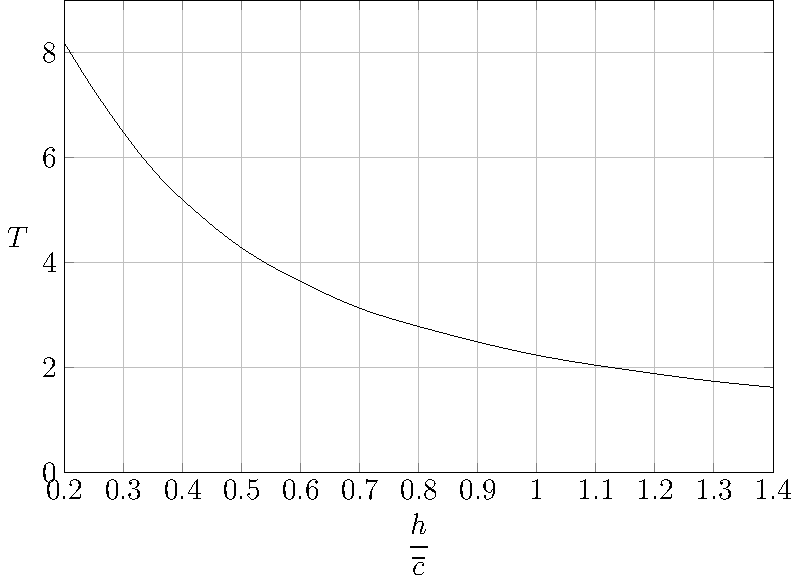
\includegraphics[height=10.5cm, keepaspectratio ]{Immagini/Capitolo2/2_13-(Delta_alpha_G)_T_vs_h_frac_overline_c} 
	\caption{Parameter accounting for variation in longitudinal velocity with ground height} % didascalia
	\label{fig:figura2_13} % etichetta per citarla nel testo
\end{figure}

\begin{figure}[H]
	%\centering
	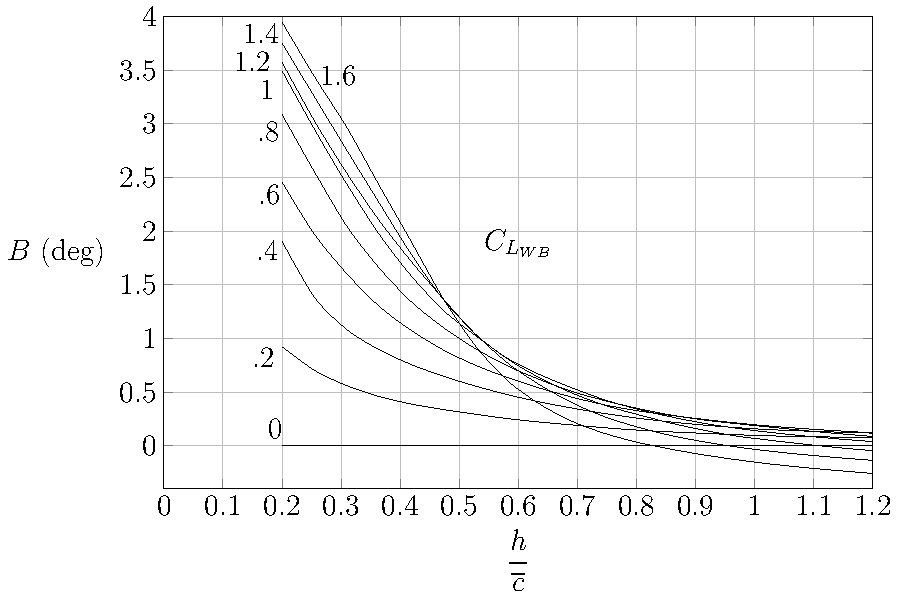
\includegraphics[height=9.5cm, keepaspectratio ]{Immagini/Capitolo2/2_14-(Delta_alpha_G)_B_vs_h_frac_overline_c_C_L_WB} 
	\caption{Parameter accounting for variation in circulation with lift and height above ground} % didascalia
	\label{fig:figura2_14} % etichetta per citarla nel testo
\end{figure}

\begin{figure}[H]
	\centering
	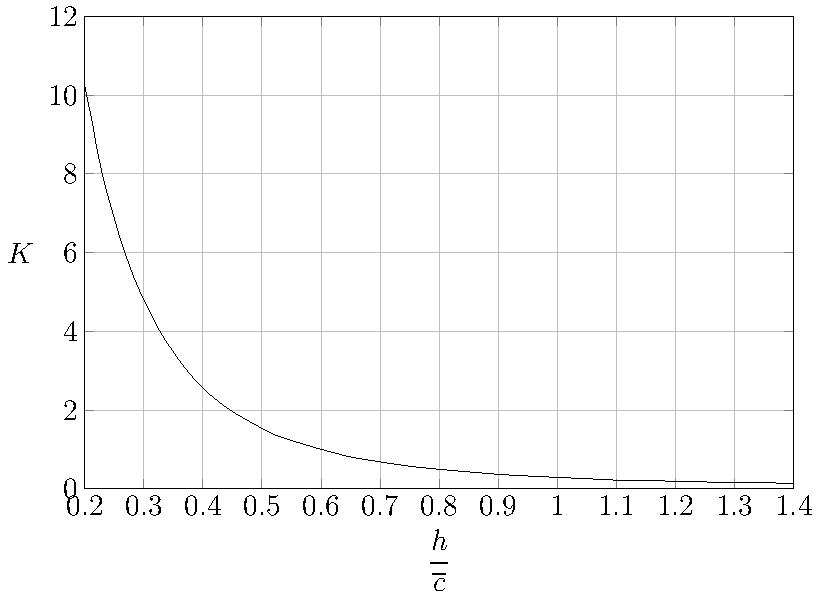
\includegraphics[height=10.5cm, keepaspectratio ]{Immagini/Capitolo2/2_15-Delta_alpha_G_K_vs_h_frac_c} 
	\caption{Parameter accounting for influence of wing thickness due to height above ground} % didascalia
	\label{fig:figura2_15} % etichetta per citarla nel testo
\end{figure}


% --------------------------------------------------------------------------------------------------------------------------------------------
% 								SEZIONE 3
% --------------------------------------------------------------------------------------------------------------------------------------------

\section{Assessment of minimum unstick speed}
The aircraft will be in the takeoff configuration at the maximum angle of attack allowed by the geometry, as shown in~\vref{fig:figura2_16}
\begin{figure}[H]
	\centering
	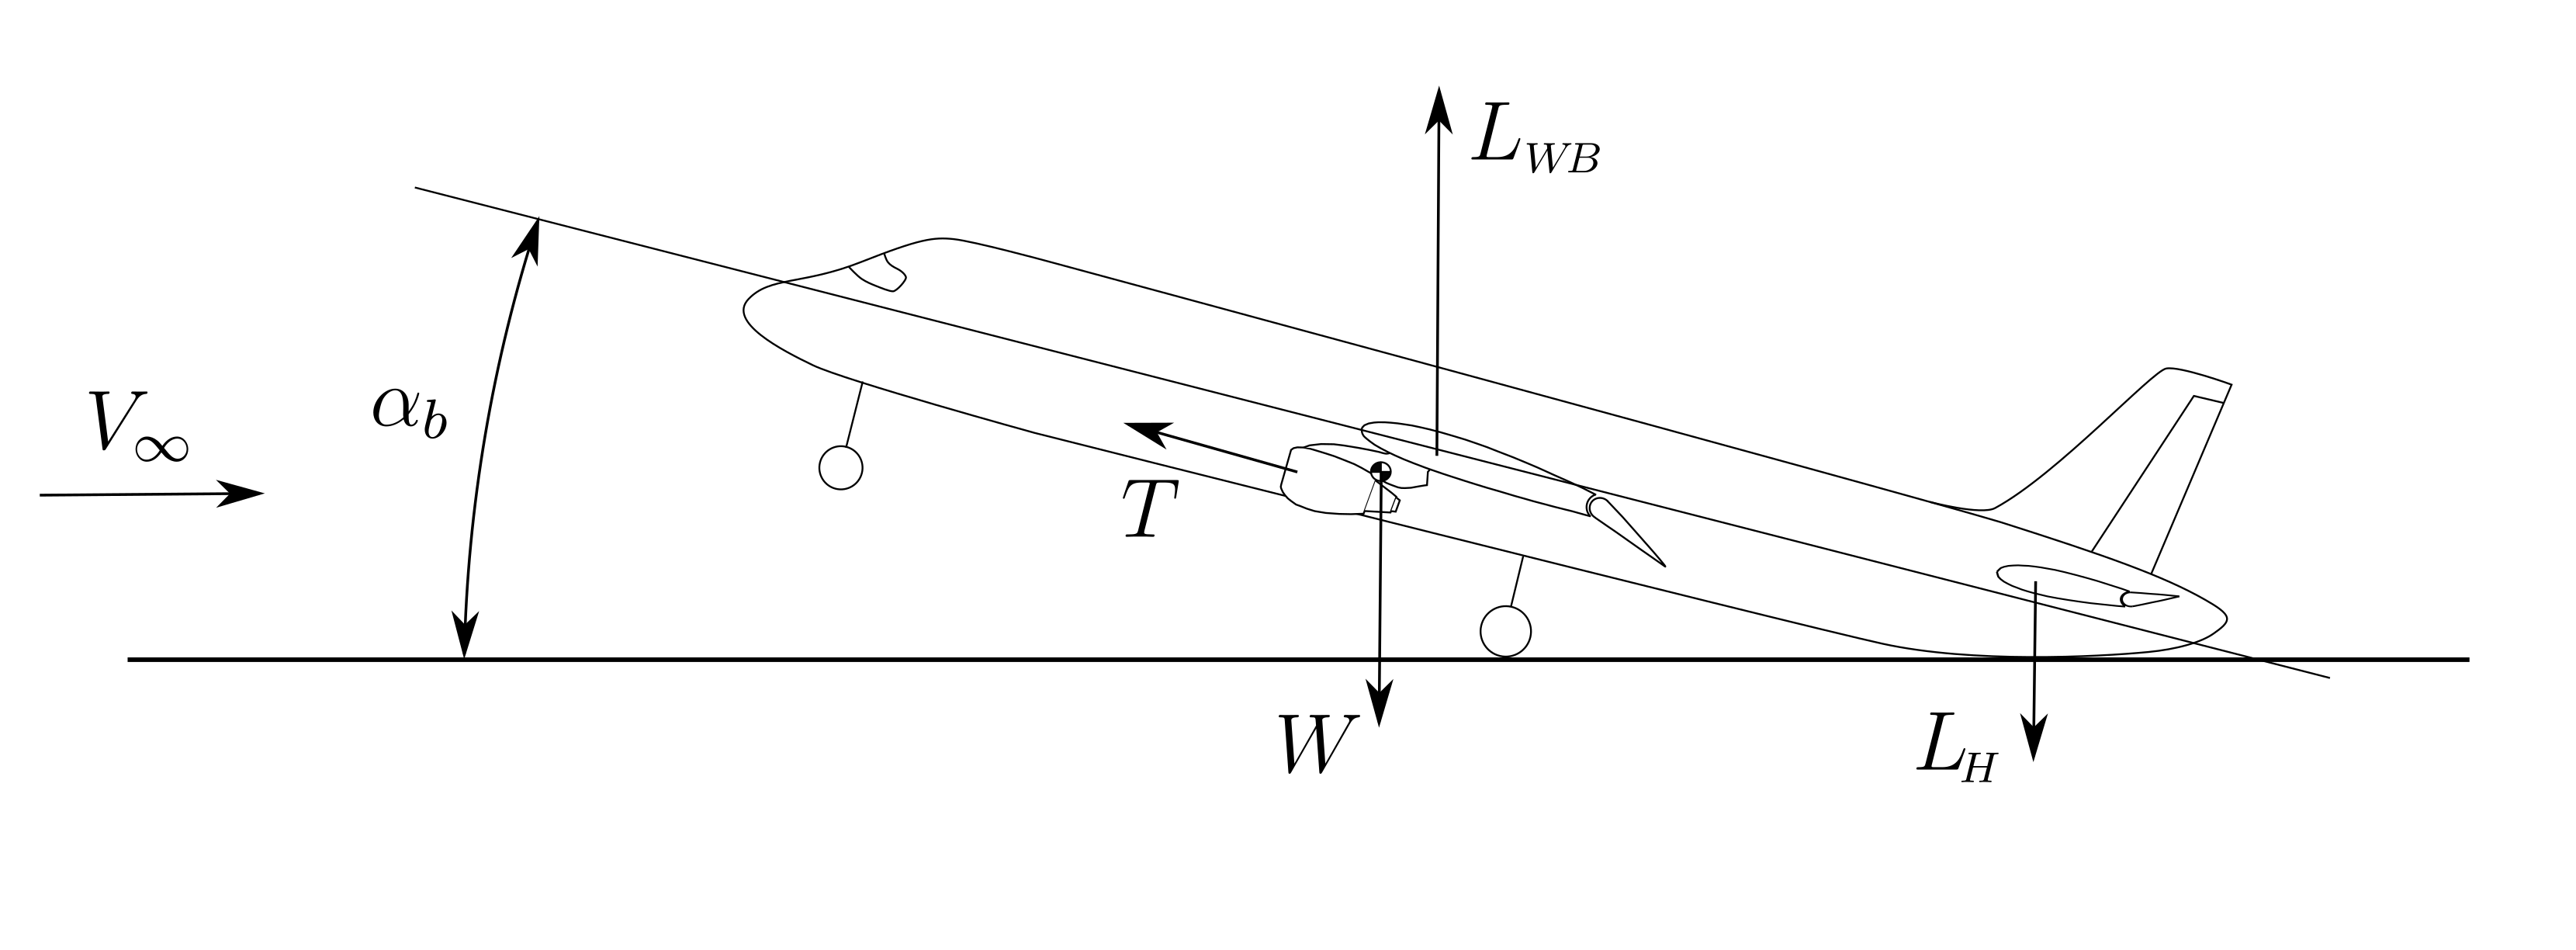
\includegraphics[height=5cm, keepaspectratio ]{Immagini/Capitolo2/2_16-aereoVmu} 
	\caption{Takeoff configuration for the assessment of VMU} % didascalia
	\label{fig:figura2_16} % etichetta per citarla nel testo
\end{figure}

Known the geometry of the fuselage can be calculated $\alpha_{W}$ and $\alpha_{H}$:

\[\alpha_{W}=\alpha_{b}+i_W\]
\[\alpha_{H}=\alpha_{b}-\varepsilon+i_H\]

The $V_{MU}$  is the speed at which the aircraft takes off in this configuration, i.e. the speed that makes the 
algebraic sum of lift (wing-body lift and horizontal tail lift) and thrust upwards component equals to the weight of the aircraft.\\
In formulas:

\begin{equation}
L_{TOT}=L_{WB}+L_H+T\sin \alpha_b=W
\label{eq:equazione2_5} % etichetta per citarla nel testo
\end{equation}
\begin{equation}
L_{TOT}=C_{L_{WB}}\frac{1}{2}\rho V_{\infty}^2S_W+C_{L_{H}}\frac{1}{2}\rho V_{\infty}^2 \eta S_H+T\sin \alpha_b=W
\label{eq:equazione2_6} % etichetta per citarla nel testo
\end{equation}
from which it is obtained:
\begin{equation}
V_{MU}=\sqrt{\frac{W-T\sin \alpha_b}{C_{L_{WB}}\frac{1}{2}\rho S_W+C{L_H}\frac{1}{2}\rho  \eta S_H}}
\label{eq:equazione2_6} % etichetta per citarla nel testo
\end{equation}
where $C_{L_{WB}}$ and $C_{L_H}$  are influenced by the ground effect. In particular there will be a new wing-body lift coefficient curve and new downwash angle as shown in section~\ref{sec:sec3}.

% !TeX program = PdfLaTeX
% !TeX root = ../Main.tex

\chapter{Results and analysis}
\label{ch3}

In this chapter is presented a case study performed on a regional turboprop of 130 pax, concerning aerodynamic characteristics, high lift devices and ground effect both on wing lift curve and on downwash angle.

\begin{figure}[H]
	\centering
	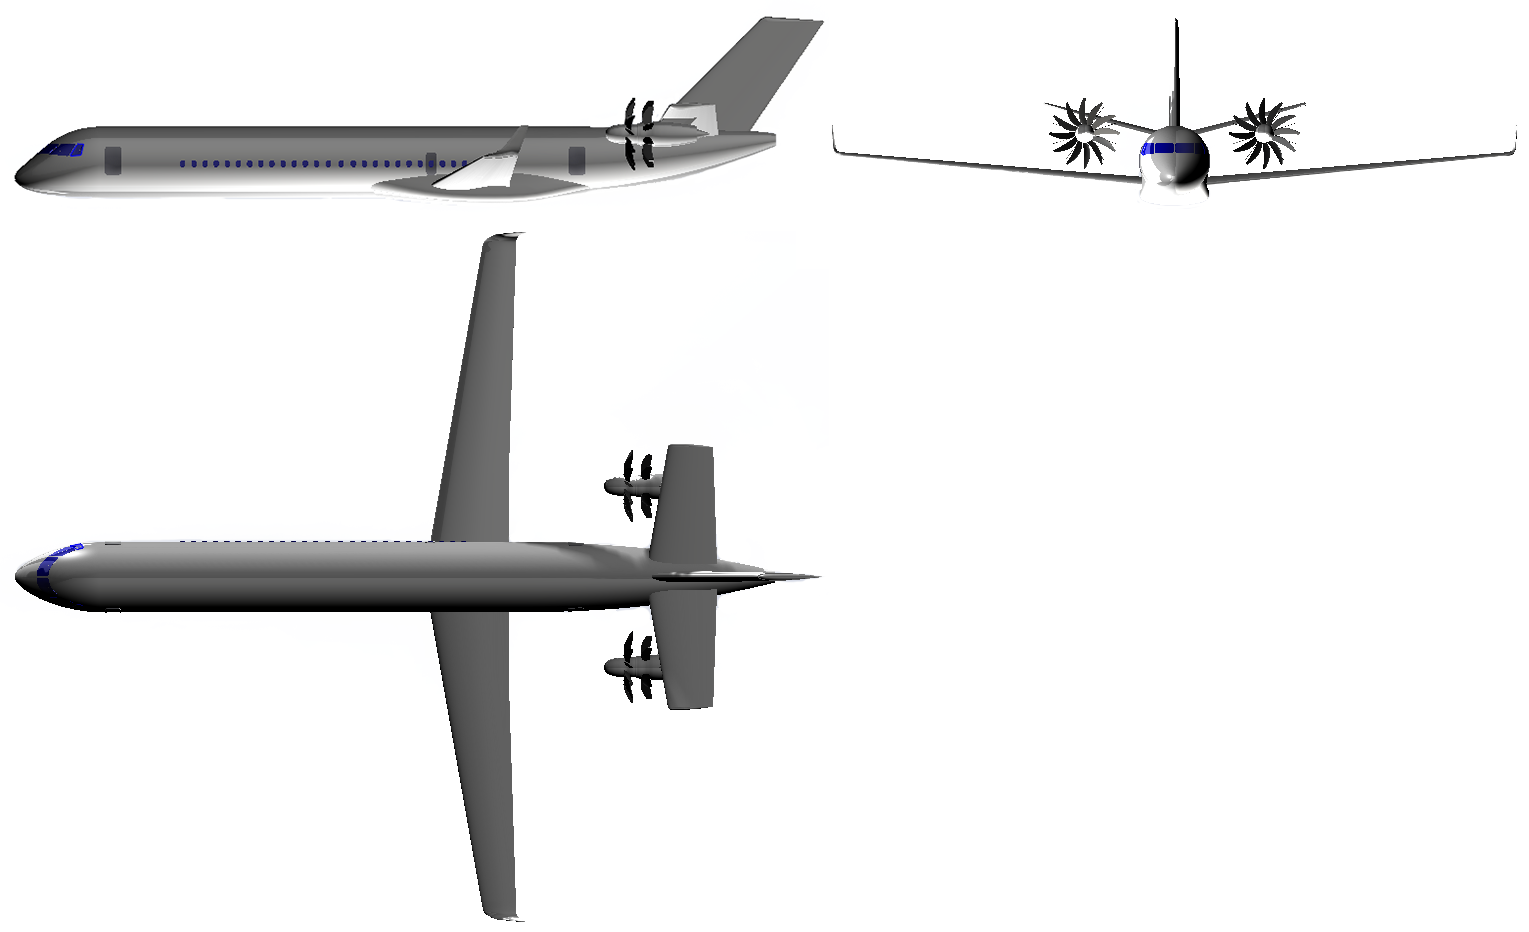
\includegraphics[height=10.5cm, keepaspectratio ]{Immagini/Capitolo3/IRON} 
	\caption{Layout of Regional Turboprop. Side, top and front section.} % didascalia
	\label{fig:figura3_0} % etichetta per citarla nel testo
\end{figure}

\begin{figure}[H]
	\centering
	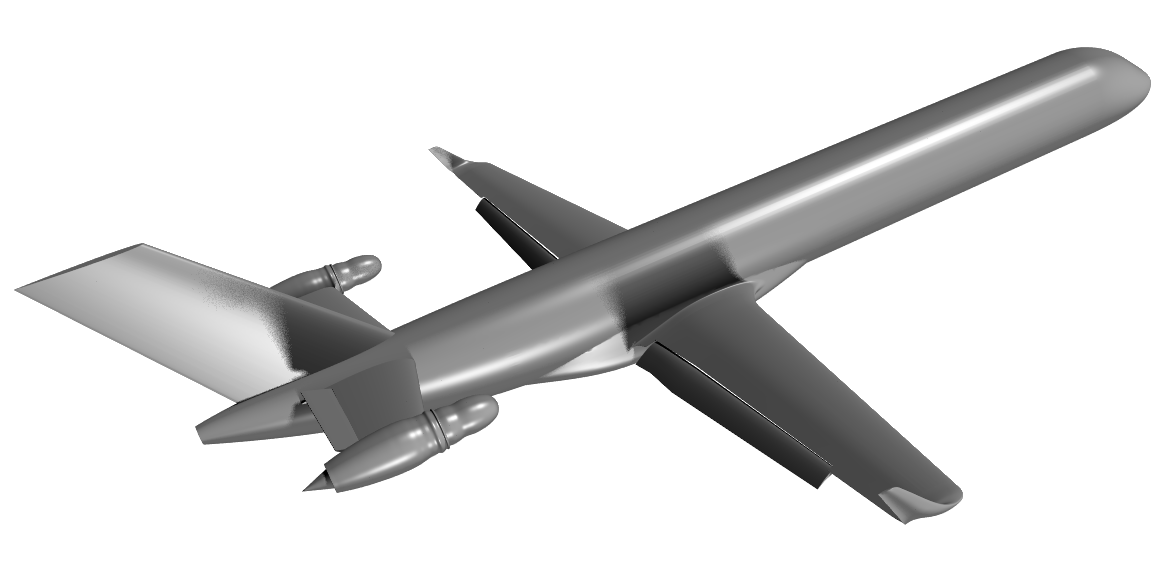
\includegraphics[height=7cm, keepaspectratio ]{Immagini/Capitolo3/IRON_TAKE_OFF} 
	\caption{Regional Turboprop rendering in takeoff configuration} % didascalia
	\label{fig:figura3_01} % etichetta per citarla nel testo
\end{figure}

\begin{table}[H]
\begin{centering}
\begin{tabular}{llc}
\toprule
\textbf{Data}&\textbf{Value} \\
\hline
\multirow{ 7}{*}{Wing}&Span	&	35.34 m	\\
& AR & 12 \\
& $C_r$ & 5.325 m \\
& $C_k$ & 4.5 m \\
& $C_t$ & 3.4 m \\
&  MAC & 3.16 m \\
& Flap type & FOWLER \\
& $\delta_{f_{TO}}$ & $\ang{25}$ \\
\hline
\multirow{4}{*}{Horizontal Tail }&Span	&	12.5 m	\\
& $C_r$ & 3.64 m \\
& $C_t$ & 2.272 m \\
& $\delta_{e_{min}}$ & $\ang{-25}$ \\
\hline
Other data&MTOW	&	51847 kg	\\
\bottomrule

\end{tabular}
\caption{Aircraft main data.}
\label{tabellaB.1}
\end{centering}
\end{table}


\begin{figure}[H]
	%\centering
	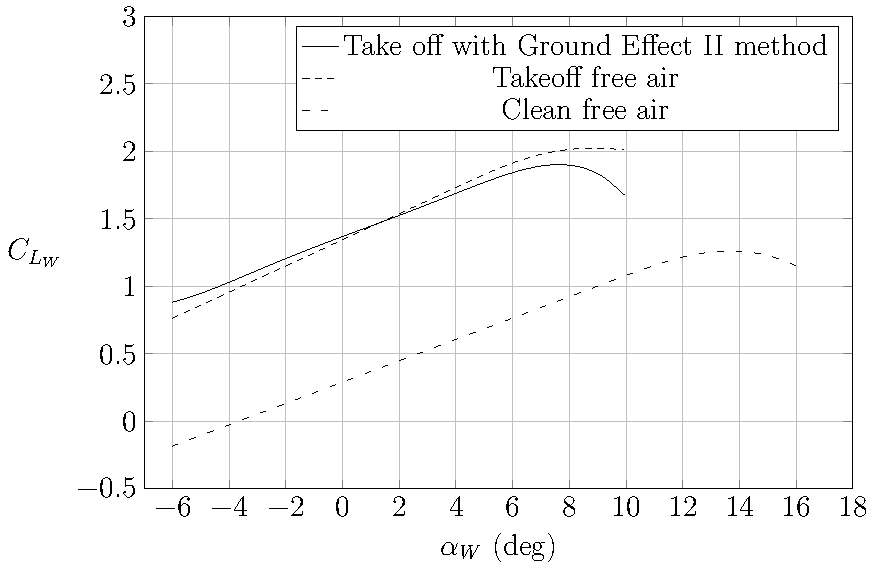
\includegraphics[height=9.5cm, keepaspectratio ]{Immagini/Capitolo3/3_1-GroundEffectOnWingLiftCurve} 
	\caption{Ground effect on wing lift curve} % didascalia
	\label{fig:figura3_1} % etichetta per citarla nel testo
\end{figure}

\begin{figure}[H]
	%\centering
	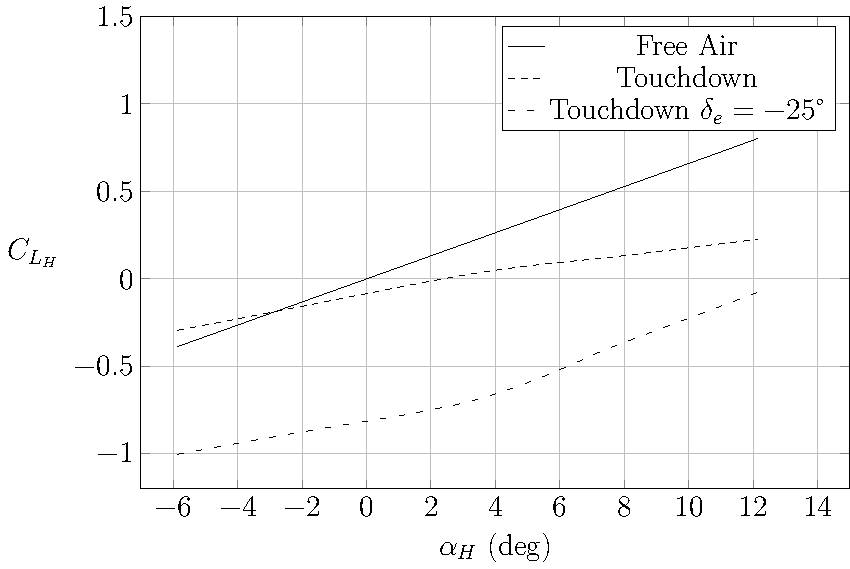
\includegraphics[height=9.5cm, keepaspectratio ]{Immagini/Capitolo3/3_2-GroundEffectOnHorizontalTailLiftCurve} 
	\caption{Ground effect on horizontal tail lift curve} % didascalia
	\label{fig:figura3_2} % etichetta per citarla nel testo
\end{figure}

\begin{figure}[H]
	%\centering
	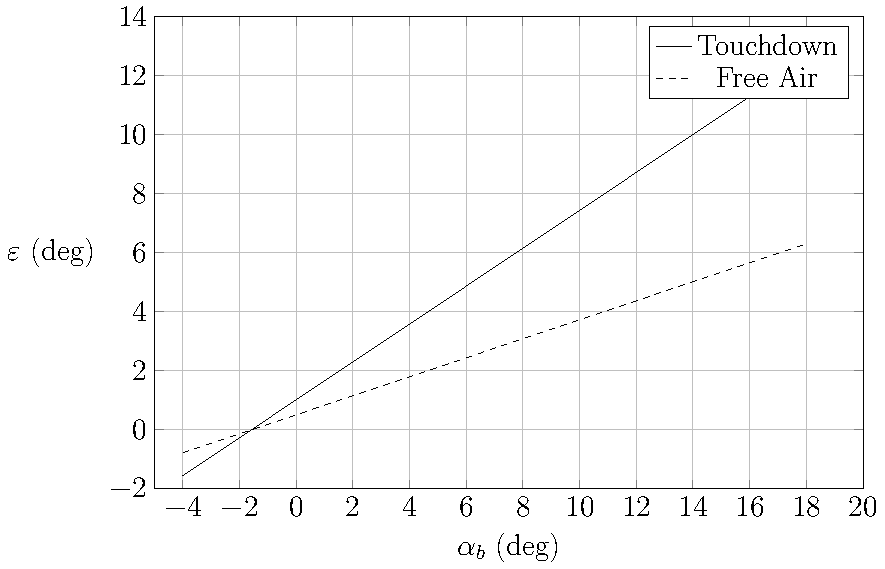
\includegraphics[height=9cm, keepaspectratio ]{Immagini/Capitolo3/3_3-GroundEffectOnDownwashAngle} 
	\caption{Ground effect on downwash angle} % didascalia
	\label{fig:figura3_3} % etichetta per citarla nel testo
\end{figure}

\begin{figure}[H]
	%\centering
	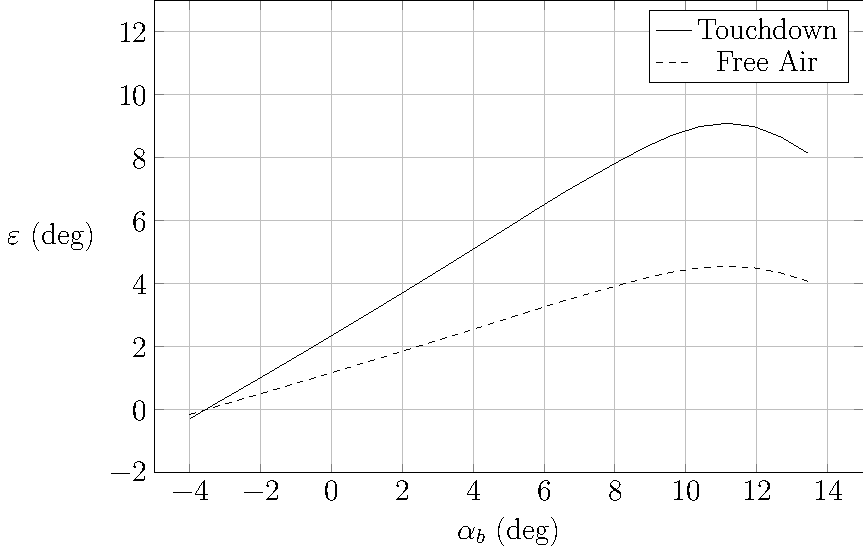
\includegraphics[height=9cm, keepaspectratio ]{Immagini/Capitolo3/3_4-GroundEffectOnDownwashAngleConsideringNonLinearEffects} 
	\caption{Ground effect on downwash angle considering non linear effects} % didascalia
	\label{fig:figura3_4} % etichetta per citarla nel testo
\end{figure}

% --------------------------------------------------------------------------------------------------------------------------------------------
% APPENDICI
% --------------------------------------------------------------------------------------------------------------------------------------------
\newpage
\appendix
\pagestyle{appendici}
\chapter{HDF dataset and database reader creation}
\label{app:appendice1}

In a tool for preliminary design phase of an aircraft, it's very important to have available database. It's possible to create database starting from graphics using external software. In this appendix will be explained the step required in order to digitalize the graphics, create an HDF dataset and set up the database-reader class in JPAD.

% --------------------------------------------------------------------------------------------------------------------------------------------
% SEZIONE 1
% --------------------------------------------------------------------------------------------------------------------------------------------
\section{Chart digitization}
\label{secA.1}

The first step required for create a dataset is to digitalize a chart. Often data are presented in reports and references as functional X-Y type scatter or line plots. In order to use this data, it must somehow be digitized. This is made with a MATLAB tool, such as \emph{Grabit}. Grabit is a Java program used to digitize scanned plots of functional data. This program will allow you to take a scanned image of a plot and quickly digitize values off the plot just by clicking the mouse on each data point \cite{Grabit}.

\begin{figure}[htbp]
\centering
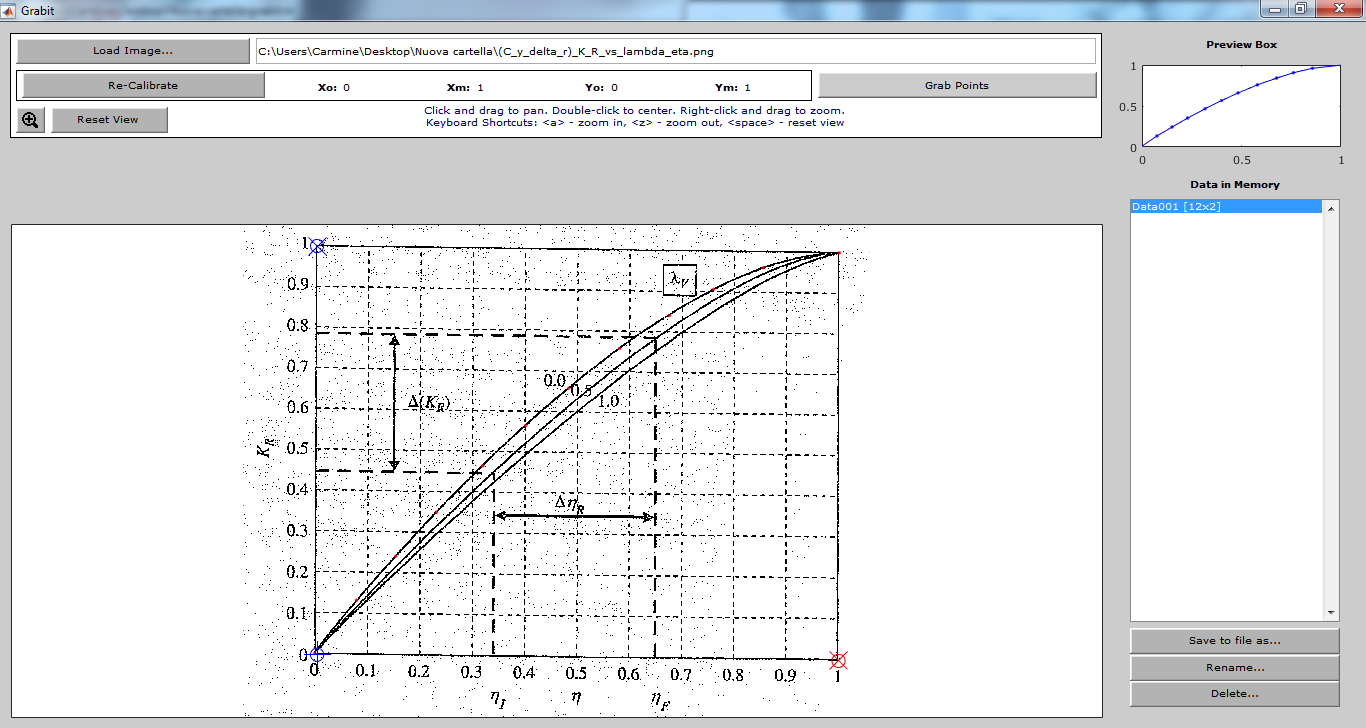
\includegraphics[height=7.9cm]{Immagini/Appendice1/Grabit} 
\caption{Chart digitization using Grabit}
\label{angles}
\end{figure} 

In order to digitize a chart, first of all it's necessary to calibrate the axis. Grabit works with both linear and logarithmic axis scales. After it's possible to digitize a curve simply click on it. The values obtained can then be saved to .mat file (MATLAB data).

% --------------------------------------------------------------------------------------------------------------------------------------------
% SEZIONE 2
% --------------------------------------------------------------------------------------------------------------------------------------------
\section{Creation of an HDF file with MATLAB}
\label{secA.2}

Obtained the .mat file from digitization is necessary to create the HDF file. After saving the imported files as .mat file, MATLAB code comes in play to manage these data and to generate the digitalized curves and the HDF dataset.  The code interpolates curves points with cubic splines in order to have more points to plot for each curve.

\bigskip
\lstset{language=Matlab}
\begin{lstlisting}[
frame=rbl,
title={\textbf{Listing A.1.} MATLAB script for creating the HDF database},
label={Listing}
]
clear; close all; clc;
%% Load data file generated by Grabit
% https://it.mathworks.com/matlabcentral/fileexchange/7173-grabit

fileBaseNames = {'KR_vs_lambda_eta_00', 'KR_vs_lambda_eta_05', 'KR_vs_lambda_eta_10'};
nPoints       = 21;
xx            = linspace(0.0, 1.0, nPoints);

for kFile = 1:length(fileBaseNames)
    
    s = load(fileBaseNames{kFile}, '-mat');

    %% Allocate imported array to column variable names
    x{kFile}        = s.(fileBaseNames{kFile})(:, 1);
    x{kFile}(1)     = 0.0;
    x{kFile}(end)   = 1.0;
    
    y{kFile}        = s.(fileBaseNames{kFile})(:, 2);
    y{kFile}(1)     = 0.0;
    y{kFile}(end)   = 1.0;
    
    %% Smoothing
    pp(kFile)       = csaps(x{kFile}, y{kFile}, 0.999999);
    c{kFile}        = ppval(pp(kFile), xx');
    data(:,kFile)   = c{kFile};
    data(1,kFile)   = 0.0;
    data(end,kFile) = 1.0;

    plot(xx', data(:,kFile), '-*');
    hold on
end
xlabel('$\eta$','interpreter','latex');
ylabel('$K_r$','interpreter','latex');
title('Span factor between rudder and vertical tail');
axis([0 1 0 1]);
legend('0.0','0.5','1.0');

%% Output to HDF
taperRatios = [0.0 0.5 1.0]';
etas        = xx';

hdfFileName = 'C_y_delta_r_K_R_vs_lambda_eta.h5';

if(exist(hdfFileName, 'file'))
    fprintf('file %s exists, deleting and creating a new one\n', hdfFileName);
    delete(hdfFileName)
else
    fprintf('Creating new file %s\n', hdfFileName);
end

h5create(hdfFileName, '/(C_y_delta_r)_K_R_vs_lambda_eta/data', size(data'));
h5write(hdfFileName, '/(C_y_delta_r)_K_R_vs_lambda_eta/data', data');

h5create(hdfFileName, '/(C_y_delta_r)_K_R_vs_lambda_eta/var_0', size(taperRatios'));
h5write(hdfFileName, '/(C_y_delta_r)_K_R_vs_lambda_eta/var_0', taperRatios');

h5create(hdfFileName, '/(C_y_delta_r)_K_R_vs_lambda_eta/var_1', size(etas'));
h5write(hdfFileName, '/(C_y_delta_r)_K_R_vs_lambda_eta/var_1', etas');
\end{lstlisting}

\newpage
This script draws the graph after digitization (see figure~\vref{plotmatlab}). In this way it's possible to compare the initial graph and the digitized one.

\begin{figure}[htbp]
\centering
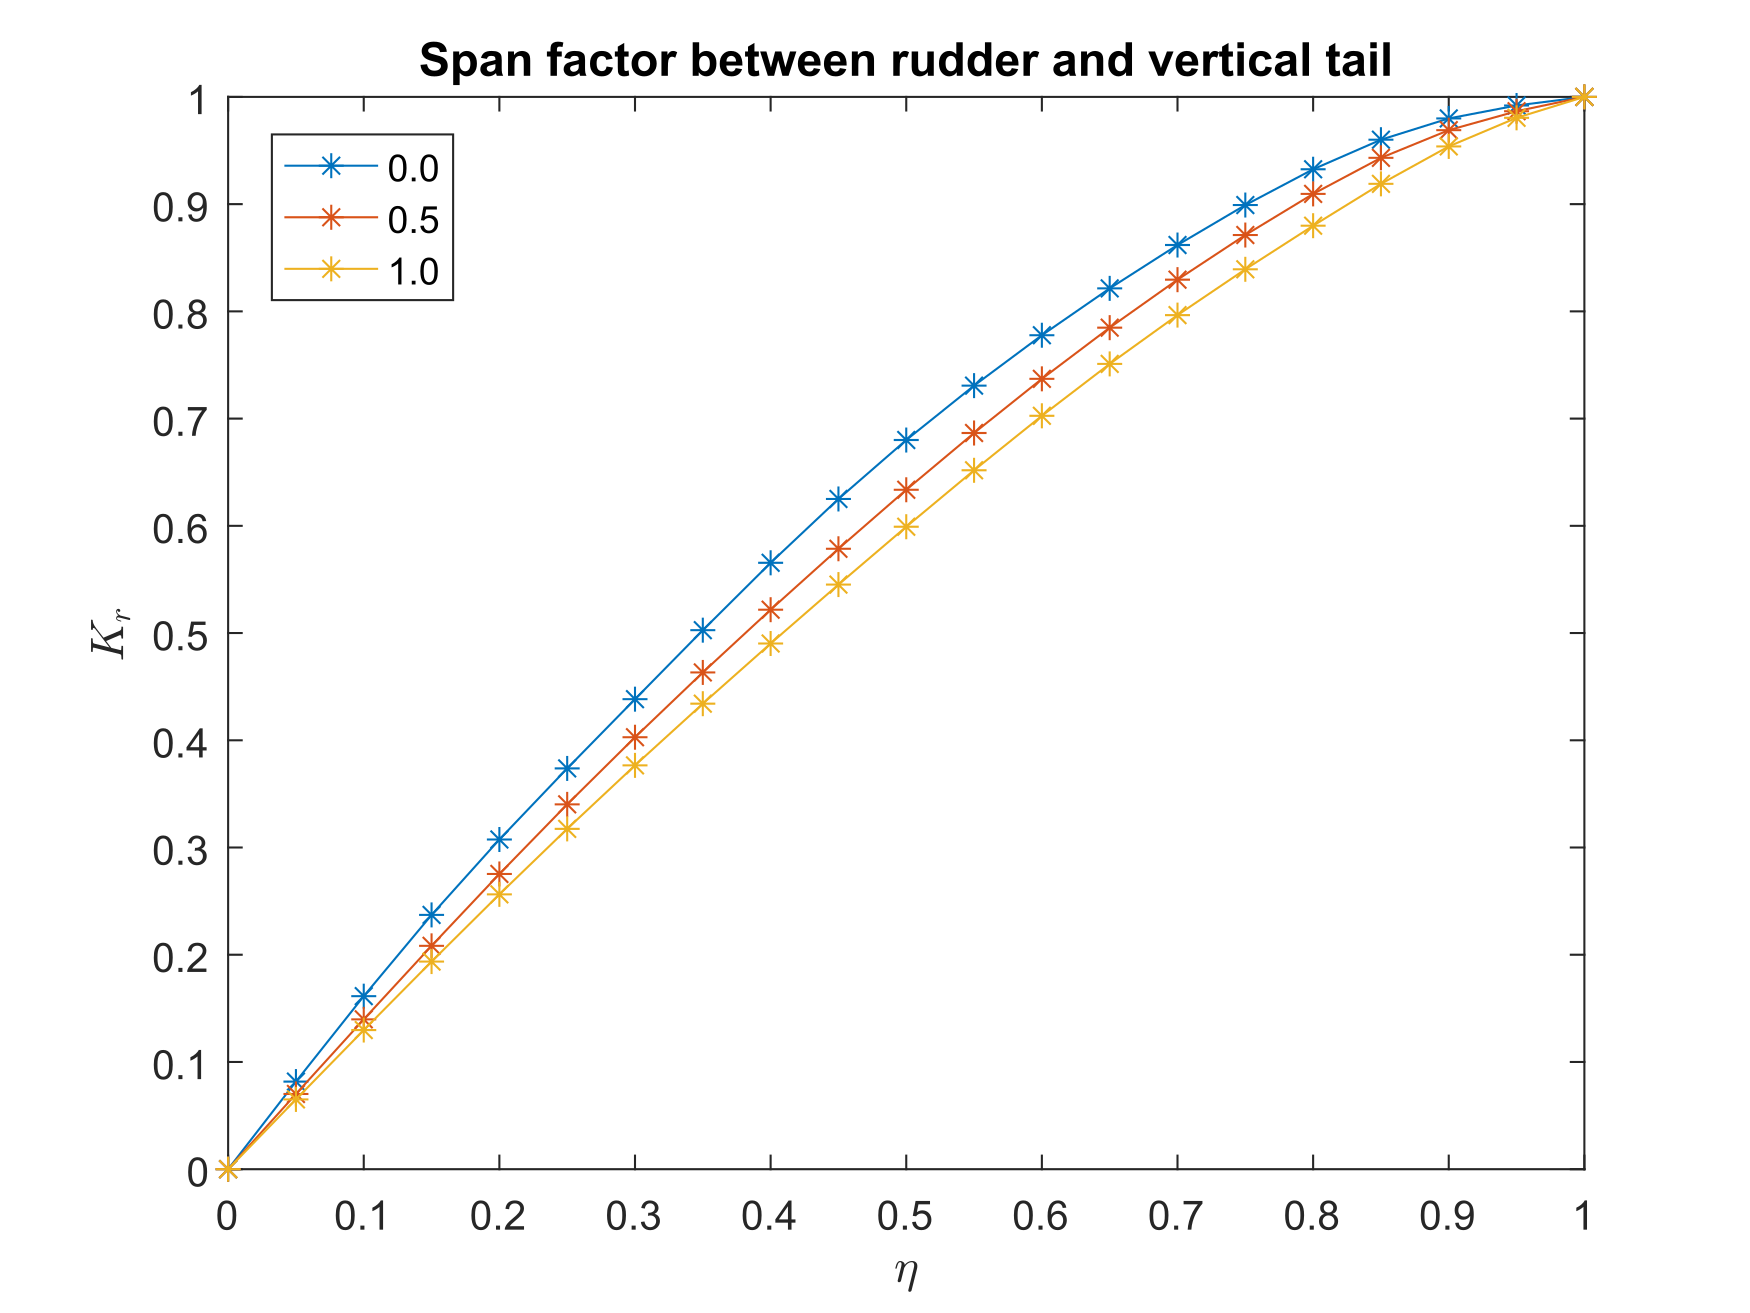
\includegraphics[height=9cm]{Immagini/Appendice1/plotmatlab}
\caption{Chart digitization plot}
\label{plotmatlab}
\end{figure} 

Having created the .h5 file it is necessary to import it in database using \emph{HDFView} \cite{HDF} and to set up the database reader implementing in specific class the variable declaration of an interpolating function starting from the .h5 file. In conclusion the getter method has to be defined.

\begin{figure}[H]
\centering
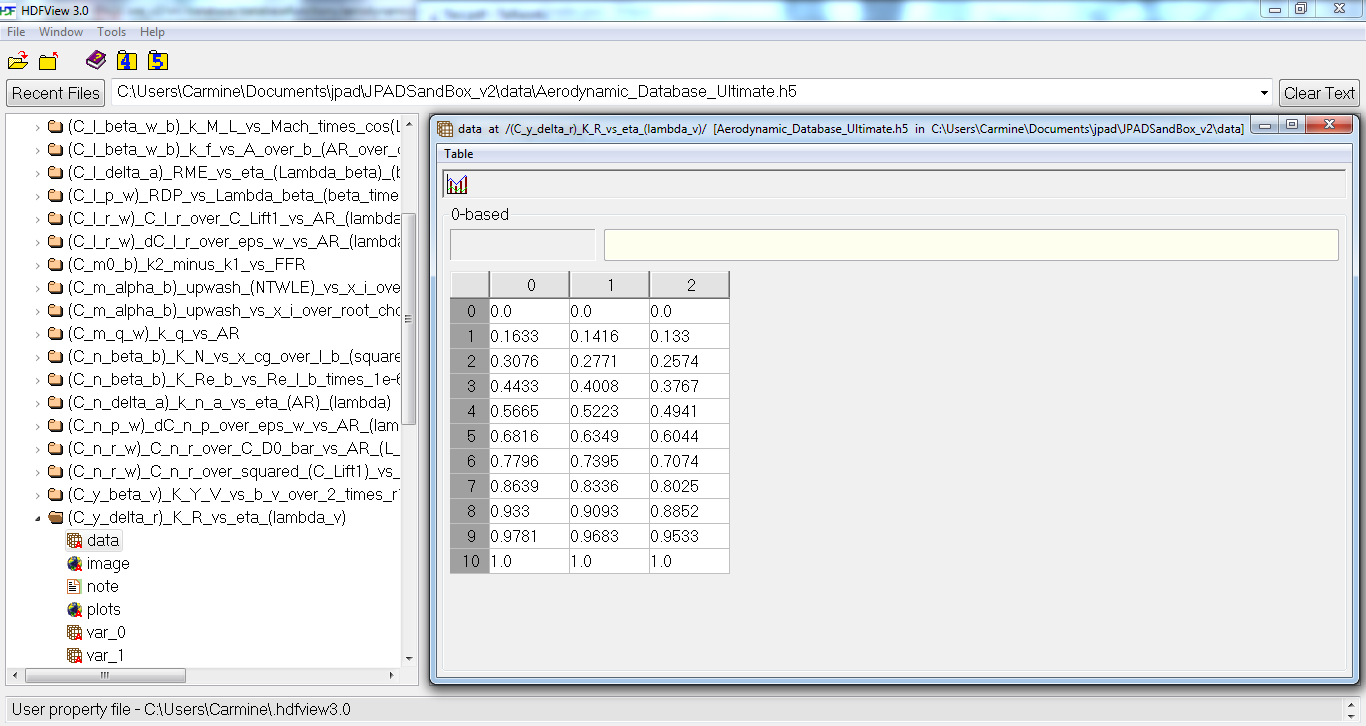
\includegraphics[width=\textwidth]{Immagini/Appendice1/HDF} 
\caption{Chart digitization using Grabit}
\label{HDF}
\end{figure} 

\newpage
\lstset{language=Java}
\begin{lstlisting}[
frame=rbl,
title={\textbf{Listing A.2.} Java extract from database reader class},
label={Listing}
]
public class AerodynamicDatabaseReader{

	private MyInterpolatingFunction C_y_delta_r_K_R_vs_eta_lambda_v;

	public AerodynamicDatabaseReader
	(String databaseFolderPath, String databaseFileName) {
		C_y_delta_r_K_R_vs_eta_lambda_v
		= database.interpolate2DFromDatasetFunction
		("(C_y_delta_r)_K_R_vs_eta_(lambda_v)");
	}

	public double getCYDeltaRKRVsEtaLambdaV(
			double taperRatio,	// var0
			double eta		// var1
			) {
		return C_y_delta_r_K_R_vs_eta_lambda_v.valueBilinear(
				eta,		// var1
				taperRatio	// var0
				);
	}
}
\end{lstlisting}
\newpage
\thispagestyle{empty}

% --------------------------------------------------------------------------------------------------------------------------------------------
% LISTA DEI SIMBOLI E GLOSSARIO
% --------------------------------------------------------------------------------------------------------------------------------------------
\backmatter
\pagestyle{backmatter}
\glsaddall
\glossarystyle{list}
\markboth{}{}
\cleardoublepage
\printglossary[type=symbols]

% --------------------------------------------------------------------------------------------------------------------------------------------
% BIBLIOGRAFIA
% --------------------------------------------------------------------------------------------------------------------------------------------
\printbibliography[heading=bibintoc]

% --------------------------------------------------------------------------------------------------------------------------------------------
% FINE DEL DOCUMENTO
% --------------------------------------------------------------------------------------------------------------------------------------------
\newpage\null\thispagestyle{empty}
\end{document}